\chapter{State-Based Drift Detection}
\label{chap:approach}
In this chapter, we present our state-based framework and thereby answer \ref{item:intro:rq_states}. The input is an event log according to Definition~\ref{def:prelim:event_log}. The output consists of intra-case, resource and inter-case states and, for each perspective, a drift signal over time. A high value of this signal indicates a concept drift.

\textcite{berti2025ocel} compute execution states of objects: They encode each event as a vector and concatenate the vectors of consecutive events of an object in sliding windows. A PCA compresses these windows, and a SOM maps them onto its cells, which are the states. We transfer these steps from objects to cases and additionally apply them to time windows to obtain resource and inter-case states. A fourth step turns the states into drift signals.

Figure~\ref{fig:approach:overview} shows the four steps with their inputs and outputs:
\begin{enumerate}
	\item \emph{Feature extraction} (Section~\ref{sec:approach:features}): For each perspective, the event log yields a feature matrix $X \in \R^{m \times n}$. In the intra-case perspective, each row describes an event, and in the resource and inter-case perspectives a feature window.
	\item \emph{Scaling and dimensionality reduction} (Section~\ref{sec:approach:reduction}): Scaling and PCA compress $X$ into a matrix $Z \in \R^{m \times d}$ with $d \le n$ principal components.
	\item \emph{Clustering into states} (Section~\ref{sec:approach:clustering}): A SOM, k-means or DBSCAN assigns a cluster to each row of $Z$. Each cluster is a state.
	\item \emph{Drift signals} (Section~\ref{sec:approach:drift_signals}): For each signal window, we compare the distribution of the states of its rows with a reference, e.g., the previous signal window, using a divergence. The divergence is the drift score of the signal window, and the drift signal is the time series of the drift scores.
\end{enumerate}

The three perspectives pass through the steps separately. Thus, each perspective has its own states and its own drift signal. Each section of this chapter covers one step and contains one subsection per perspective. Chapter~\ref{chap:impl} introduces the AI-assisted analysis. It is not a step of the pipeline, but interprets the results of the pipeline with an LLM.

\begin{figure}[tb]
	\centering
	\begin{tikzpicture}[font=\small, >={Stealth},
			lane/.style={draw, rounded corners=2pt, fill=black!6, align=left, text width=2.8cm, minimum height=1.3cm},
			stage/.style={draw, rounded corners=2pt, fill=black!6, align=center, text width=2cm, minimum height=4.3cm},
			head/.style={align=center, text width=2.7cm, font=\small\bfseries},
			io/.style={align=center, text width=2.7cm}]
		% column headers, one per section of the chapter
		\node[head, text width=1.3cm] at (0.65, 4.25) {Input};
		\node[head] at (3.5, 4.25) {Feature extraction (Section~\ref{sec:approach:features})};
		\node[head] at (6.7, 4.25) {Scaling and dimensionality reduction (Section~\ref{sec:approach:reduction})};
		\node[head] at (9.45, 4.25) {Clustering into states (Section~\ref{sec:approach:clustering})};
		\node[head] at (12.2, 4.25) {Drift signals (Section~\ref{sec:approach:drift_signals})};
		% input
		\node[draw, align=center, text width=1.1cm, minimum height=1.2cm] (log) at (0.65, 1.3) {Event log~$L$};
		% feature extraction differs per perspective
		\node[lane] (fi) at (3.5, 2.75) {\textbf{Intra-case:} one row per event};
		\node[lane] (fr) at (3.5, 1.3) {\textbf{Resource:} one row per feature window};
		\node[lane] (fn) at (3.5, -0.15) {\textbf{Inter-case:} one row per feature window};
		% the later steps use the same techniques, but run separately per perspective
		\node[stage] (dr) at (6.7, 1.3) {Scaling and PCA};
		\node[stage] (cl) at (9.45, 1.3) {SOM, \mbox{k-means} or DBSCAN};
		\node[stage] (ds) at (12.2, 1.3) {State distribution per signal window, divergence from a reference};
		\foreach \lane in {fi, fr, fn} {
			\draw[->] (log.east) -- (\lane.west);
			\draw[->] (\lane.east) -- (\lane.east -| dr.west);
			\draw[->] (\lane.east -| dr.east) -- (\lane.east -| cl.west);
			\draw[->] (\lane.east -| cl.east) -- (\lane.east -| ds.west);
		}
		% output of each step
		\node[head, text width=1.3cm] at (0.65, -1.75) {Output};
		\node[io] at (3.5, -1.75) {feature matrix $X \in \R^{m \times n}$};
		\node[io] at (6.7, -1.75) {compressed \mbox{matrix} $Z \in \R^{m \times d}$};
		\node[io] at (9.45, -1.75) {one state per row of~$Z$};
		\node[io] at (12.2, -1.75) {drift signal: one drift score per signal window};
	\end{tikzpicture}
	\caption[Overview of the state-based framework]{%
		Overview of the state-based framework. The event log $L$ passes through the four steps separately for each perspective, shown by the three arrows between two steps. The bottom row gives the output of each step, and each column is one section of this chapter.}
	\label{fig:approach:overview}
\end{figure}

The framework uses calendar windows (Definition~\ref{def:prelim:windows}) in two roles, which Definition~\ref{def:approach:window_roles} introduces formally:
\begin{itemize}
	\item \emph{Feature windows:} In the resource and inter-case perspectives, a feature vector describes the events of a feature window, e.g., of one day. The intra-case perspective has no feature windows.
	\item \emph{Signal windows:} The drift signal has one drift score per signal window. A signal window summarizes the states of the events or feature windows that lie in it and is at least as long as a feature window.
\end{itemize}

As a running example, we generate the event log $L_3$ with 4,920 cases and 24,600 events from the year 2020 using Rheon (Chapter~\ref{chap:rheon}). Its cases execute the five activities $a$ to $e$, four resources handle them, and the amount is a numerical case attribute. $L_3$ contains one sudden drift per perspective (Table~\ref{tab:approach:running_drifts}):
\begin{itemize}
	\item \emph{Control-flow:} Before the drift, all cases follow the process tree ${\rightarrow}(a,\allowbreak {\rightarrow}({\rightarrow}(b, c),\allowbreak {\rightarrow}(d, e)))$. Afterwards, they follow ${\rightarrow}({\rightarrow}(a,\allowbreak {\wedge}(b, c)),\allowbreak {\wedge}(d, e))$, i.e., $b$ and $c$ as well as $d$ and $e$ swap their order.
	\item \emph{Resource:} Each activity gets a new dominant resource.
	\item \emph{Inter-case:} The mean amount of the cases rises from 1000 to 2500 euros.
\end{itemize}
Table~\ref{tab:approach:running_log} shows one case before and one case after all drifts. We choose the lengths of the feature and signal windows per perspective in each section.

\begin{table}[tb]
	\centering
	\caption[Drifts of the running example]{%
		The three sudden drifts of the running example $L_3$. The position is the fraction of the year 2020 at which Rheon injects the drift.}
	\label{tab:approach:running_drifts}
	\small
	\begin{tabular}{@{}rlll@{}}
		\toprule
		Position & Drift point          & Perspective & Drift type             \\
		\midrule
		0.25     & Apr.~1, 2020, 06:00  & Intra-case  & \texttt{control\_flow} \\
		0.50     & July~1, 2020, 12:00  & Resource    & \texttt{reassignment}  \\
		0.75     & Sep.~30, 2020, 18:00 & Inter-case  & \texttt{amount}        \\
		\bottomrule
	\end{tabular}
\end{table}

\begin{table}[tb]
	\centering
	\caption[Excerpt of the running example]{%
		Two cases of the running example $L_3$, case~1 before and case~3711 after all drifts. Identifiers are abbreviated, timestamps are completion times, durations are in minutes and amounts in euros. Case~3711 swaps $b$ and $c$ as well as $d$ and $e$, its events are executed by the new dominant resources of their activities, and its amount is higher.}
	\label{tab:approach:running_log}
	\small
	\begin{tabular}{@{}llllrrl@{}}
		\toprule
		Case & Activity & Timestamp     & Resource         & Duration & Amount  & Region            \\
		\midrule
		1    & $a$      & Jan.~1, 00:17 & \texttt{res\_01} & 17.57    & 780.51  & \texttt{region\_4} \\
		1    & $b$      & Jan.~1, 00:49 & \texttt{res\_01} & 27.98    & 780.51  & \texttt{region\_4} \\
		1    & $c$      & Jan.~1, 01:40 & \texttt{res\_02} & 39.92    & 780.51  & \texttt{region\_4} \\
		1    & $d$      & Jan.~1, 02:16 & \texttt{res\_01} & 19.22    & 780.51  & \texttt{region\_4} \\
		1    & $e$      & Jan.~1, 02:57 & \texttt{res\_04} & 25.82    & 780.51  & \texttt{region\_4} \\
		\addlinespace
		3711 & $a$      & Oct.~2, 01:07 & \texttt{res\_03} & 26.25    & 2476.48 & \texttt{region\_4} \\
		3711 & $c$      & Oct.~2, 01:49 & \texttt{res\_03} & 31.48    & 2476.48 & \texttt{region\_4} \\
		3711 & $b$      & Oct.~2, 02:19 & \texttt{res\_02} & 28.48    & 2476.48 & \texttt{region\_4} \\
		3711 & $e$      & Oct.~2, 03:00 & \texttt{res\_02} & 28.42    & 2476.48 & \texttt{region\_4} \\
		3711 & $d$      & Oct.~2, 03:45 & \texttt{res\_02} & 27.78    & 2476.48 & \texttt{region\_4} \\
		\bottomrule
	\end{tabular}
\end{table}

\section{Feature Extraction}
\label{sec:approach:features}
Feature extraction translates an event log into numbers. It is the only step that reads the event log, so a drift that no feature captures stays invisible in all following steps. In the intra-case perspective, a row of the feature matrix describes an event by the prefix of its case. In the other two perspectives, it describes a feature window by the events that lie in it.

The feature groups use the notation for vectors and statistics of Section~\ref{sec:prelim:maths}, and time differences are in minutes (Section~\ref{sec:prelim:windows}).

\begin{definition}[Feature and Signal Windows]
	\label{def:approach:window_roles}
	Let $o \in \U{time}$ be an origin, and let $\Delta_f, \Delta_s \in \R$ with $0 < \Delta_f \le \Delta_s$.
	\begin{itemize}
		\item The feature windows are the calendar windows with the origin $o$ and the length $\Delta_f$, and the signal windows are those with the origin $o$ and the length $\Delta_s$ (Definition~\ref{def:prelim:windows}).
		\item A feature window $w = [t, t + \Delta_f)$ lies in the signal window that contains its start $t$. An event lies in the signal window that contains its timestamp.
	\end{itemize}
\end{definition}

Thus, each feature window lies in exactly one signal window. If $\Delta_s$ is a multiple of $\Delta_f$, the feature window lies completely in it. Otherwise, some feature windows reach into the next signal window, and the signal windows contain different numbers of feature windows (Figure~\ref{fig:approach:windows}).

\begin{figure}[tb]
	\centering
	\definecolor{sigA}{RGB}{0,114,178}
	\definecolor{sigB}{RGB}{230,159,0}
	\definecolor{sigC}{RGB}{0,158,115}
	\definecolor{sigD}{RGB}{204,121,167}
	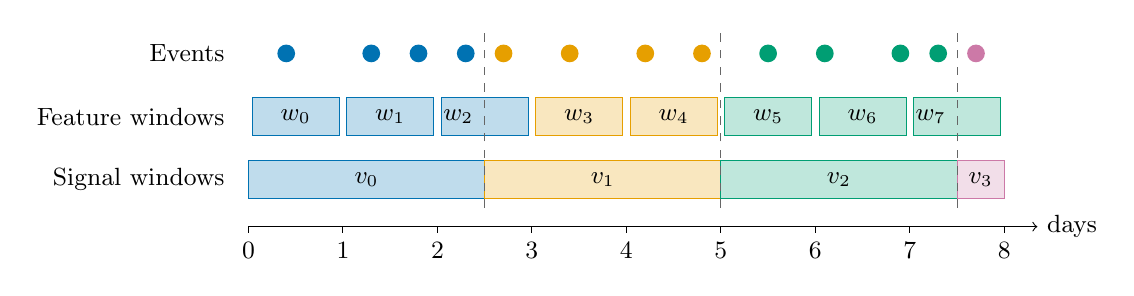
\begin{tikzpicture}[font=\small, x=1.2cm, y=0.8cm]
		\node[anchor=east] at (-0.15, 2) {Events};
		\node[anchor=east] at (-0.15, 1) {Feature windows};
		\node[anchor=east] at (-0.15, 0) {Signal windows};
		% signal windows of 2.5 days, the last one cut at day 8
		\foreach \a/\b/\c/\n in {0/2.5/sigA/0, 2.5/5/sigB/1, 5/7.5/sigC/2} {
			\draw[fill=\c!25, draw=\c] (\a, -0.3) rectangle (\b, 0.3);
			\node at ({(\a + \b) / 2}, 0) {$v_{\n}$};
		}
		\draw[fill=sigD!25, draw=sigD] (7.5, -0.3) rectangle (8, 0.3);
		\node at (7.75, 0) {$v_3$};
		% feature windows of one day, each in the color of the signal window of its start
		% the labels of w_2 and w_7 sit left of the signal window boundary that crosses them
		\foreach \k/\c/\l in {0/sigA/0.5, 1/sigA/0.5, 2/sigA/0.22, 3/sigB/0.5, 4/sigB/0.5, 5/sigC/0.5, 6/sigC/0.5, 7/sigC/0.22} {
			\draw[fill=\c!25, draw=\c] (\k + 0.04, 0.7) rectangle (\k + 0.96, 1.3);
			\node at (\k + \l, 1) {$w_{\k}$};
		}
		% boundaries of the signal windows through all rows
		\foreach \x in {2.5, 5, 7.5}
			\draw[dashed, black!60] (\x, -0.45) -- (\x, 2.4);
		% events, each in the color of the signal window of its timestamp
		\foreach \t/\c in {0.4/sigA, 1.3/sigA, 1.8/sigA, 2.3/sigA, 2.7/sigB, 3.4/sigB, 4.2/sigB, 4.8/sigB, 5.5/sigC, 6.1/sigC, 6.9/sigC, 7.3/sigC, 7.7/sigD}
			\fill[\c] (\t, 2) circle (3.2pt);
		% time axis
		\draw[->] (0, -0.75) -- (8.35, -0.75) node[right] {days};
		\foreach \d in {0, ..., 8}
			\draw (\d, -0.75) -- (\d, -0.85) node[below] {\d};
	\end{tikzpicture}
	\caption[Feature windows and signal windows]{%
		Feature windows of $\Delta_f = 1$~day and signal windows of $\Delta_s = 2.5$~days with the same origin at day~0. Each feature window has the color of the signal window that contains its start, each event the color of the signal window that contains its timestamp, and dashed lines are the boundaries of the signal windows. Since 2.5 is no multiple of 1, $w_2$ and $w_7$ reach into the next signal window, and $v_0$, $v_1$ and $v_2$ hold three, two and three feature windows. The event after 2.5 days lies in $v_1$, whereas its feature window $w_2$ lies in $v_0$.}
	\label{fig:approach:windows}
\end{figure}

\begin{definition}[Predecessors, Gaps and Feature Windows of an Event Log]
	\label{def:approach:windows}
	Let $L = (E, \pi, \preceq)$ be an event log, and let feature windows of the length $\Delta_f$ be given (Definition~\ref{def:approach:window_roles}).
	\begin{itemize}
		\item For a case with the events $e_1 \preceq \dots \preceq e_l$ (Definition~\ref{def:prelim:trace}), $\mathit{prev}_L(e_i) = e_{i-1}$ for $1 < i \le l$ is the predecessor of $e_i$. The first event of a case has no predecessor, so $\mathit{prev}_L \in E \pto E$.
		\item For $e \in \dom(\mathit{prev}_L)$, $\mathit{gap}_L(e) = \pi_{\mathit{time}}(e) - \pi_{\mathit{time}}(\mathit{prev}_L(e))$ is the gap between $e$ and its predecessor.
		\item For a feature window $w$, $E^w_L = \Set{e \in E \given \pi_{\mathit{time}}(e) \in w}$ is the set of its events.
		\item $W_L$ are the feature windows from the window of the first to the window of the last event of $L$ in chronological order, including those without events.
	\end{itemize}
\end{definition}

\begin{definition}[Feature Extraction]
	\label{def:approach:feature_extraction}
	Let $L = (E, \pi, \preceq)$ be an event log with the rows $s_1, \dots, s_m$, i.e., the events in the order $\preceq$ in the intra-case perspective and the feature windows $W_L$ (Definition~\ref{def:approach:windows}) in the other two perspectives.
	\begin{itemize}
		\item A feature group $f$ computes from $L$ a vector $f_L(s) \in \R^p$ for each row $s$, e.g., with one entry per activity.
		\item For the chosen feature groups $f^1, \dots, f^g$, $\mathbf{x}_s = (f^1_L(s), \dots, f^g_L(s)) \in \R^n$ is the feature vector of the row $s$.
		\item Together, the feature vectors of all rows form the feature matrix $X \in \R^{m \times n}$ with the rows $\mathbf{x}_{s_1}^\top, \dots, \mathbf{x}_{s_m}^\top$ (Section~\ref{sec:prelim:pca}).
	\end{itemize}
\end{definition}

The following subsections define the feature groups of each perspective that we use in this thesis. The framework also works with only a part of these feature groups or with self-defined ones. In the dashboard, users choose the feature groups (Section~\ref{sec:impl:dashboard}), and our library kairo is flexible for custom features (Section~\ref{sec:impl:kairo}).

For each perspective, a figure shows to which Rheon drift types our feature groups respond.

\subsection{Intra-Case Perspective}
\label{sec:approach:features:intra}
The intra-case features describe each event $e$ by the prefix of its case, i.e., by the activities of the case up to and including $e$. Since a prefix has a variable length, the feature groups abstract it to different degrees. A multiset of the prefix ignores the order of the activities, a set additionally ignores their frequencies, and the last activity ignores all earlier ones. The current and the past activities adopt the encoding of \textcite{berti2025ocel}, which concatenates the one-hot vectors of the activities of consecutive events.

\begin{definition}[Intra-Case Features]
	\label{def:approach:intra}
	Let $L = (E, \pi, \preceq)$ be an event log with the activities $A_L = \Set{\pi_{\mathit{act}}(e) \given e \in E} = \Set{a_1, \dots, a_p}$, let $D_L = \Set{d_1, \dots, d_u} \subseteq A_L \times A_L$ be the set of directly-follows pairs that occur in a trace of $L$, and let $h \in \N_0$. Let $e_k$ be the $k$-th of $l$ events of a case and $\sigma = \mathit{prefix}_L(e_k)$ (Definition~\ref{def:prelim:trace}). The built-in feature groups of $e_k$ are:
	\begin{itemize}
		\item \emph{Activity frequencies} (\texttt{act\_freqs}): the share of each activity among the first $k$ events of the case:
		      \[
			      \mathit{freq}_L(e_k) = (\partial_{\mathit{multiset}}(\sigma)(a_1), \dots, \partial_{\mathit{multiset}}(\sigma)(a_p)) / k.
		      \]
		\item \emph{Directly-follows counts} (\texttt{df\_counts}): how often each directly-follows pair occurs in the prefix:
		      \[
			      \mathit{dfc}_L(e_k) = (\mathit{df}(\sigma)(d_1), \dots, \mathit{df}(\sigma)(d_u)).
		      \]
		\item \emph{Activity set} (\texttt{act\_set}): $\mathit{set}_L(e_k) = \sum_{a_i \in \partial_{\mathit{set}}(\sigma)} \mathit{onehot}_p(i)$, i.e., a 1 for each activity that occurs in the prefix.
		\item \emph{Case progress} (\texttt{case\_progress}): $\mathit{progress}_L(e_k) = k / l$.
		\item \emph{Current activity} (\texttt{current\_act}): $\mathit{cur}_L(e_k) = \mathit{onehot}_p(i)$ for $\sigma(k) = a_i$.
		\item \emph{Past activities} (\texttt{past\_acts}): $\mathit{past}^h_L(e_k) = (\mathbf{y}_1, \dots, \mathbf{y}_h)$, i.e., the activities of the $h$ previous events of the case, with $\mathbf{y}_j = \mathit{onehot}_p(i)$ for $j < k$ and $\sigma(k - j) = a_i$, and $\mathbf{y}_j = \mathbf{0}$ otherwise.
	\end{itemize}
\end{definition}

\noindent\emph{Properties:}
\begin{itemize}[beginpenalty=10000]
	\item The feature groups only read the activities of a case. Only the directly-follows counts and the past together with the current activity capture the order.
	\item The case progress knows the length of the whole case and thus requires a completely recorded event log (Section~\ref{sec:intro_ssec:probs}).
	\item An activity or a directly-follows pair that only occurs after a drift gets its own column, which is 0 before the drift.
\end{itemize}

\begin{table}[tb]
	\centering
	\caption[Intra-case feature vectors of the running example]{%
		Two rows of the intra-case feature matrix of $L_3$ with three feature groups: the third events of case~1 before and of case~3711 after the control-flow drift (Table~\ref{tab:approach:running_log}). The activity columns are in the order $a$ to $e$, the directly-follows columns in the order $a \to b$, $a \to c$, $b \to c$, $b \to d$, $b \to e$, $c \to b$, $c \to d$, $c \to e$, $d \to e$ and $e \to d$. Only the directly-follows counts and the current activity differ between the two events.}
	\label{tab:approach:features_intra}
	\small
	\begin{tabular}{@{}lll@{}}
		\toprule
		Feature group           & Case 1, prefix $\seq{a, b, c}$            & Case 3711, prefix $\seq{a, c, b}$         \\
		\midrule
		Activity frequencies    & $(1/3, 1/3, 1/3, 0, 0)$                   & $(1/3, 1/3, 1/3, 0, 0)$                   \\
		Directly-follows counts & $(1, 0, 1, 0, 0, 0, 0, 0, 0, 0)$ & $(0, 1, 0, 0, 0, 1, 0, 0, 0, 0)$ \\
		Current activity        & $(0, 0, 1, 0, 0)$                & $(0, 1, 0, 0, 0)$                \\
		\bottomrule
	\end{tabular}
\end{table}

\begin{example}
	\label{ex:approach:intra}
	For the intra-case features of $L_3$, we choose the activity frequencies, the directly-follows counts and the current activity. With five activities and ten directly-follows pairs, a feature vector has $5 + 10 + 5 = 20$ entries. The prefixes $\seq{a, b, c}$ and $\seq{a, c, b}$ in Table~\ref{tab:approach:features_intra} contain the same activities in a different order, so only the directly-follows counts and the current activity differ.
\end{example}

% Styles and legend shared by the three figures that map the feature groups of a
% perspective to the drift types of Rheon. The drift types keep the same rows in all
% three figures, and drift types that reach the same feature groups lie next to each other
\definecolor{perspIntra}{RGB}{0,114,178}
\definecolor{perspResource}{RGB}{230,159,0}
\definecolor{perspInter}{RGB}{0,158,115}
\tikzset{
	mapfeature/.style={anchor=east, inner sep=2pt},
	mapdrift/.style={anchor=west, rounded corners=1.5pt, line width=1pt, inner sep=2.5pt, minimum width=2.8cm, text height=1.6ex, text depth=0.4ex},
	mapunused/.style={text=black!40},
	mapdirect/.style={line width=0.9pt},
	mapindirect/.style={line width=0.9pt, dashed, black!55},
}
% the legend, its first row at the height #1
\newcommand*{\maplegend}[1]{%
	\draw[mapdirect] (-0.2, #1) -- ++(0.7, 0) node[right] (l1) {direct response};
	\draw[mapindirect] ([xshift=0.4cm]l1.east) -- ++(0.7, 0) node[right, text=black] (l2) {response through a side effect};
	\node[mapdrift, minimum width=0pt, draw=black!30, mapunused, right=0.4cm of l2] {no response};
	\node[anchor=west] (p0) at (-0.2, #1 + 1.1) {Perspective of a drift type:};
	\node[mapdrift, minimum width=0pt, draw=perspIntra, fill=perspIntra!12, right=0.3cm of p0] (p1) {intra-case};
	\node[mapdrift, minimum width=0pt, draw=perspResource, fill=perspResource!12, right=0.3cm of p1] (p2) {resource};
	\node[mapdrift, minimum width=0pt, draw=perspInter, fill=perspInter!12, right=0.3cm of p2] {inter-case};
}

\begin{figure}[tb]
	\centering
	\begin{tikzpicture}[font=\small, y=-0.65cm]
		% the nine drift types of Rheon, in the same rows in all three figures
		\node[mapdrift, draw=perspResource!45, mapunused] (wl) at (9.6, 0) {\texttt{workload}};
		\node[mapdrift, draw=perspInter!45, mapunused] (ar) at (9.6, 1) {\texttt{arrival\_rate}};
		\node[mapdrift, draw=perspInter!45, mapunused] (wt) at (9.6, 2) {\texttt{waiting\_time}};
		\node[mapdrift, draw=perspResource!45, mapunused] (du) at (9.6, 3) {\texttt{duration}};
		\node[mapdrift, draw=perspResource!45, mapunused] (ps) at (9.6, 4) {\texttt{pool\_size}};
		\node[mapdrift, draw=perspIntra, fill=perspIntra!12] (cf) at (9.6, 5) {\texttt{control\_flow}};
		\node[mapdrift, draw=perspResource!45, mapunused] (ra) at (9.6, 6) {\texttt{reassignment}};
		\node[mapdrift, draw=perspInter!45, mapunused] (am) at (9.6, 7) {\texttt{amount}};
		\node[mapdrift, draw=perspInter!45, mapunused] (rg) at (9.6, 8) {\texttt{region}};
		% intra-case feature groups
		\foreach \i/\lab in {0/Activity frequencies, 1/Directly-follows counts, 2/Activity set, 3/Case progress, 4/Current activity, 5/Past activities}
			\node[mapfeature] (f\i) at (5.6, 8 * \i / 5) {\lab};
		\foreach \f/\d in {0/cf, 1/cf, 2/cf, 3/cf, 4/cf, 5/cf}
			\draw[mapdirect] (f\f.east) -- (\d.west);
		\maplegend{9.5}
	\end{tikzpicture}
	\caption[Intra-case feature groups and the drift types they respond to]{%
		The Rheon drift types (right) to which the intra-case feature groups (left) of Definition~\ref{def:approach:intra} respond. Only control-flow drifts reach them.}
	\label{fig:approach:features_intra}
\end{figure}

Figure~\ref{fig:approach:features_intra} shows the mapping of the intra-case features. The directly-follows counts and the past activities capture a control-flow drift most directly (Section~\ref{sec:rheon:drifts}), and the other feature groups only if the drift changes the activities or the length of the cases. Among the Rheon drift types, a change of the intra-case states therefore only indicates control-flow drifts.

\subsection{Resource Perspective}
\label{sec:approach:features:resource}
The resource features describe each feature window by how the resources work in it. \textcite{adams2023explainable} list, among others, the workload, service times, waiting times and handovers as features of time windows. The activity-resource shares correspond to the probabilities $P(a \to r)$ with which \textcite{khraiwesh2027window} describe which resource $r$ executes an activity $a$. \textcite{klijn2024multi} use handovers of cases between actors as a feature for drifts in the actor perspective.

\begin{definition}[Resource Features]
	\label{def:approach:resource}
	Let $L = (E, \pi, \preceq)$ be an event log with a resource for each event, let $\mathit{prev}_L$, $\mathit{gap}_L$, $E^w_L$ and $W_L$ be as in Definition~\ref{def:approach:windows}, and let $R_L = \Set{\pi_{\mathit{res}}(e) \given e \in E} = \Set{r_1, \dots, r_q}$ be the set of resources.
	\begin{itemize}
		\item $H_L = \Set{e \in \dom(\mathit{prev}_L) \given \pi_{\mathit{res}}(\mathit{prev}_L(e)) \neq \pi_{\mathit{res}}(e)}$ is the set of handovers, i.e., of the events whose predecessor another resource executed, and $H^w_L = H_L \cap E^w_L$.
		\item For $w \in W_L$ and $r \in R_L$, $E^{w,r}_L = \Set{e \in E^w_L \given \pi_{\mathit{res}}(e) = r}$ is the set of the events of $r$ in $w$.
		\item $P_L = \Set{p_1, \dots, p_u}$ is the set of pairs of an activity and a resource, and $Q_L = \Set{q_1, \dots, q_v}$ the set of pairs of a handing-over and a receiving resource that occur in $L$.
	\end{itemize}
	For a feature window $w \in W_L$, the feature groups we use are:
	\begin{itemize}
		\item \emph{Events per resource} (\texttt{res\_events}):
		      \[
			      \mathit{events}_L(w) = (\abs{E^{w,r_1}_L}, \dots, \abs{E^{w,r_q}_L}).
		      \]
		\item \emph{Active cases per resource} (\texttt{res\_cases}):
		      \[
			      \mathit{cases}_L(w) = (x_1, \dots, x_q) \quad\text{with}\quad x_i = \abs{\Set{\pi_{\mathit{case}}(e) \given e \in E^{w,r_i}_L}}.
		      \]
		\item \emph{Mean event duration per resource} (\texttt{res\_durations}), if each event has a duration:
		      \[
			      \mathit{dur}_L(w) = (x_1, \dots, x_q) \quad\text{with}\quad x_i = \mathit{mean}(\MultiSet{\pi_{\mathit{duration}}(e) \given e \in E^{w,r_i}_L}).
		      \]
		\item \emph{Mean wait into resource} (\texttt{res\_waits}):
		      \[
			      \mathit{wait}_L(w) = (x_1, \dots, x_q) \quad\text{with}\quad x_i = \mathit{mean}(\MultiSet{\mathit{gap}_L(e) \given e \in H^w_L \cap E^{w,r_i}_L}).
		      \]
		\item \emph{Activity-resource event shares} (\texttt{act\_res\_shares}): the share of the events of $a$ in $w$ that $r$ executes, i.e., $\mathit{ar}_L(w) = (x_1, \dots, x_u)$, where for $p_i = (a, r)$:
		      \[
			      x_i = \mathit{ratio}(\abs{\Set{e \in E^{w,r}_L \given \pi_{\mathit{act}}(e) = a}}, \abs{\Set{e \in E^w_L \given \pi_{\mathit{act}}(e) = a}}).
		      \]
		\item \emph{Handover shares} (\texttt{handover\_shares}): the share of the handovers of $r$ in $w$ that go to $r'$, i.e., $\mathit{ho}_L(w) = (x_1, \dots, x_v)$, where for $q_i = (r, r')$:
		      \[
			      \begin{aligned}
				      x_i = \mathit{ratio}( & \abs{\Set{e \in H^w_L \cap E^{w,r'}_L \given \pi_{\mathit{res}}(\mathit{prev}_L(e)) = r}}, \\
				                      & \abs{\Set{e \in H^w_L \given \pi_{\mathit{res}}(\mathit{prev}_L(e)) = r}}).
			      \end{aligned}
		      \]
	\end{itemize}
\end{definition}

\noindent\emph{Properties:}
\begin{itemize}[beginpenalty=10000]
	\item The counts grow with the number of cases per unit of time. The shares are normalized per activity or per handing-over resource and thus independent of this number.
	\item A handover counts in the feature window of the receiving event $e$. Since the timestamps are completion times, $\mathit{gap}_L(e)$ covers the waiting time before $e$ and the duration of $e$.
\end{itemize}

\begin{table}[tb]
	\centering
	\caption[Resource feature vectors of the running example]{%
		Rows of the resource feature matrix of $L_3$ with feature windows of one day and two feature groups, around the resource drift on July~1, 2020. The table is transposed: each column is the feature vector of a feature window. Of the activity-resource event shares, only those of activity $a$ for \texttt{res\_01} and \texttt{res\_03} are shown.}
	\label{tab:approach:features_resource}
	\small
	\begin{tabular}{@{}lrrrr@{}}
		\toprule
		Feature                      & June~29 & June~30 & July~2 & July~3 \\
		\midrule
		\multicolumn{5}{@{}l}{\emph{Events per resource}}                    \\
		\quad \texttt{res\_01}        & 45      & 40      & 3      & 4      \\
		\quad \texttt{res\_02}        & 16      & 16      & 32     & 45     \\
		\quad \texttt{res\_03}        & 2       & 3       & 26     & 33     \\
		\quad \texttt{res\_04}        & 18      & 18      & 5      & 9      \\
		\addlinespace
		\multicolumn{5}{@{}l}{\emph{Activity-resource event shares}}         \\
		\quad $a$ by \texttt{res\_01} & 0.94    & 0.88    & 0.08   & 0.05   \\
		\quad $a$ by \texttt{res\_03} & 0.00    & 0.06    & 0.83   & 0.79   \\
		\bottomrule
	\end{tabular}
\end{table}

\begin{example}
	\label{ex:approach:resource}
	For the resource features of $L_3$, we choose feature windows of one day and the feature groups events per resource and activity-resource event shares. With four resources and 20 pairs of an activity and a resource, a feature vector has $4 + 20 = 24$ entries. Before the drift, \texttt{res\_01} is the dominant resource of $a$, $b$ and $d$. Afterwards, \texttt{res\_02} and \texttt{res\_03} take over these activities (Table~\ref{tab:approach:features_resource}).
\end{example}

\begin{figure}[tb]
	\centering
	\begin{tikzpicture}[font=\small, y=-0.65cm]
		% the nine drift types of Rheon, in the same rows in all three figures
		\node[mapdrift, draw=perspResource, fill=perspResource!12] (wl) at (9.6, 0) {\texttt{workload}};
		\node[mapdrift, draw=perspInter, fill=perspInter!12] (ar) at (9.6, 1) {\texttt{arrival\_rate}};
		\node[mapdrift, draw=perspInter, fill=perspInter!12] (wt) at (9.6, 2) {\texttt{waiting\_time}};
		\node[mapdrift, draw=perspResource, fill=perspResource!12] (du) at (9.6, 3) {\texttt{duration}};
		\node[mapdrift, draw=perspResource, fill=perspResource!12] (ps) at (9.6, 4) {\texttt{pool\_size}};
		\node[mapdrift, draw=perspIntra, fill=perspIntra!12] (cf) at (9.6, 5) {\texttt{control\_flow}};
		\node[mapdrift, draw=perspResource, fill=perspResource!12] (ra) at (9.6, 6) {\texttt{reassignment}};
		\node[mapdrift, draw=perspInter!45, mapunused] (am) at (9.6, 7) {\texttt{amount}};
		\node[mapdrift, draw=perspInter!45, mapunused] (rg) at (9.6, 8) {\texttt{region}};
		% resource feature groups
		\foreach \i/\lab in {0/Events per resource, 1/Active cases per resource, 2/Mean event duration per resource, 3/Mean wait into resource, 4/Activity-resource event shares, 5/Handover shares}
			\node[mapfeature] (f\i) at (5.6, 8 * \i / 5) {\lab};
		\foreach \f/\d in {0/wl, 0/ps, 0/ra, 1/wl, 1/ps, 1/ra, 2/du, 2/ps, 3/wt, 4/ps, 4/ra, 5/ps, 5/ra}
			\draw[mapdirect] (f\f.east) -- (\d.west);
		\foreach \f/\d in {0/ar, 1/ar, 3/du, 3/ps, 3/ra, 5/cf}
			\draw[mapindirect] (f\f.east) -- (\d.west);
		\maplegend{9.5}
	\end{tikzpicture}
	\caption[Resource feature groups and the drift types they respond to]{%
		The Rheon drift types (right) to which the resource feature groups (left) of Definition~\ref{def:approach:resource} respond. Besides the resource drift types, they also respond to arrival rate, waiting time and control-flow drifts.}
	\label{fig:approach:features_resource}
\end{figure}

Figure~\ref{fig:approach:features_resource} shows the mapping of the resource features:
\begin{itemize}
	\item \emph{Reassignment and pool size} change which resource executes an activity and thus the counts and the shares. A pool size drift additionally scales the durations (Section~\ref{sec:rheon:drifts}) and therefore also reaches the feature groups of a duration drift.
	\item \emph{Duration:} Since a gap includes the duration of the receiving event, the waiting times also respond to duration drifts.
	\item \emph{Workload and arrival rate} both change the mean inter-arrival time in Rheon (Section~\ref{sec:rheon:generation}) and thus the counts in the same way. No resource feature distinguishes them.
	\item \emph{Control-flow:} Since resources are bound to activities, a new order of the activities also changes the handovers.
\end{itemize}

\subsection{Inter-Case Perspective}
\label{sec:approach:features:inter}
The inter-case features describe each feature window by all cases that run in it. \textcite{kraus2026steady} describe a process as a system by the number of arriving, active and completed cases per period. Similarly, \textcite{senderovich2017intra} use the number of cases running at a point in time in their coarsest inter-case encoding.

\begin{definition}[Inter-Case Features]
	\label{def:approach:inter}
	Let $L = (E, \pi, \preceq)$ be an event log, let $\mathit{prev}_L$, $\mathit{gap}_L$, $E^w_L$ and $W_L$ be as in Definition~\ref{def:approach:windows} with the length $\Delta_f$ of the feature windows, and let $\tau > 0$ be a stall threshold. Let $N_{\mathit{num}} = \Set{n_1, \dots, n_s}$ and $N_{\mathit{cat}}$ be disjoint sets of numerical and categorical case attributes of $L$ (Definition~\ref{def:prelim:event_log}) that every event has, and let $V = \Set{u_1, \dots, u_t}$ be the set of pairs $(n, v)$ of an attribute $n \in N_{\mathit{cat}}$ and one of its values $v$ in $L$. For a feature window $w = [t, t + \Delta_f) \in W_L$, our feature groups are:
	\begin{itemize}
		\item \emph{Active cases} (\texttt{active\_cases}): $\mathit{active}_L(w) = \abs{\Set{\pi_{\mathit{case}}(e) \given e \in E^w_L}}$.
		\item \emph{New arrivals} (\texttt{new\_arrivals}): $\mathit{arrivals}_L(w) = \abs{\Set{c \in C_L \given \mathit{start}_L(c) \in w}}$.
		\item \emph{Completions} (\texttt{completions}): $\mathit{completions}_L(w) = \abs{\Set{c \in C_L \given \mathit{end}_L(c) \in w}}$.
		\item \emph{Events per active case} (\texttt{events\_per\_case}):
		      \[
			      \mathit{epc}_L(w) = \mathit{ratio}(\abs{E^w_L}, \mathit{active}_L(w)).
		      \]
		\item \emph{Mean within-case gap} (\texttt{mean\_delta\_t}) and \emph{standard deviation of within-case gaps} (\texttt{std\_delta\_t}): $\mathit{gapmean}_L(w) = \mathit{mean}(G)$ and $\mathit{gapstd}_L(w) = \mathit{std}(G)$ with
		      \[
			      G = \MultiSet{\mathit{gap}_L(e) \given e \in E^w_L \cap \dom(\mathit{prev}_L)}.
		      \]
		\item \emph{Stalled cases} (\texttt{stalled\_cases}): the cases whose last event lies more than $\tau$ before the end $t + \Delta_f$ of $w$ and that still have a later event:
		      \[
			      \mathit{stalled}_L(w) = \abs{\Set{\pi_{\mathit{case}}(e) \given e \in \dom(\mathit{prev}_L) \land \pi_{\mathit{time}}(\mathit{prev}_L(e)) + \tau < t + \Delta_f < \pi_{\mathit{time}}(e)}}.
		      \]
		\item \emph{Means} (\texttt{attr\_means}) and \emph{standard deviations of numerical attributes} (\texttt{attr\_stds}) with $M_n = \MultiSet{\pi_n(e) \given e \in E^w_L}$:
		      \[
			      \begin{aligned}
				      \mathit{attrmean}_L(w) & = (\mathit{mean}(M_{n_1}), \dots, \mathit{mean}(M_{n_s})), \\
				      \mathit{attrstd}_L(w)  & = (\mathit{std}(M_{n_1}), \dots, \mathit{std}(M_{n_s})).
			      \end{aligned}
		      \]
		\item \emph{Value shares of categorical attributes} (\texttt{attr\_shares}): the share of the events in $w$ with the value $v$ of $n$, for $u_i = (n, v)$:
		      \[
			      \mathit{attrshare}_L(w) = (x_1, \dots, x_t) \quad\text{with}\quad x_i = \mathit{ratio}(\abs{\Set{e \in E^w_L \given \pi_n(e) = v}}, \abs{E^w_L}).
		      \]
	\end{itemize}
\end{definition}

\noindent\emph{Properties:}
\begin{itemize}[beginpenalty=10000]
	\item A case is active in every feature window that contains one of its events. Arrivals and completions, in contrast, count it only once.
	\item If only the number of cases per unit of time rises, the events per active case stay about the same.
	\item The stalled cases are only informative if $\tau$ is of the order of the gaps and many ends of feature windows fall into gaps.
	\item The attribute features weight events, not cases. Without chosen case attributes, drifts in the case attributes stay invisible.
\end{itemize}

\begin{table}[tb]
	\centering
	\caption[Inter-case feature vectors of the running example]{%
		Rows of the inter-case feature matrix of $L_3$ with feature windows of 12~hours and four feature groups, around the inter-case drift on September~30, 2020, 18:00. The table is transposed: each column is the feature vector of a feature window, given by its start. Gaps are in minutes and amounts in euros.}
	\label{tab:approach:features_inter}
	\small
	\begin{tabular}{@{}lrrrr@{}}
		\toprule
		Feature              & Sep.~29, 12:00 & Sep.~30, 00:00 & Oct.~1, 00:00 & Oct.~1, 12:00 \\
		\midrule
		Active cases         & 6              & 9              & 7             & 8             \\
		New arrivals         & 5              & 7              & 4             & 7             \\
		Mean within-case gap & 50.66          & 45.22          & 44.29         & 42.50         \\
		Mean of the amount   & 912.46         & 931.22         & 2375.81       & 2599.66       \\
		\bottomrule
	\end{tabular}
\end{table}

\begin{example}
	\label{ex:approach:inter}
	For the inter-case features of $L_3$, we choose shorter feature windows of 12~hours and the feature groups active cases, new arrivals, mean within-case gap and the mean of the amount. Only the mean amount jumps at the drift, while the other features fluctuate from window to window (Table~\ref{tab:approach:features_inter}).
\end{example}

\begin{figure}[tb]
	\centering
	\begin{tikzpicture}[font=\small, y=-0.65cm]
		% the nine drift types of Rheon, in the same rows in all three figures
		\node[mapdrift, draw=perspResource, fill=perspResource!12] (wl) at (9.6, 0) {\texttt{workload}};
		\node[mapdrift, draw=perspInter, fill=perspInter!12] (ar) at (9.6, 1) {\texttt{arrival\_rate}};
		\node[mapdrift, draw=perspInter, fill=perspInter!12] (wt) at (9.6, 2) {\texttt{waiting\_time}};
		\node[mapdrift, draw=perspResource, fill=perspResource!12] (du) at (9.6, 3) {\texttt{duration}};
		\node[mapdrift, draw=perspResource, fill=perspResource!12] (ps) at (9.6, 4) {\texttt{pool\_size}};
		\node[mapdrift, draw=perspIntra, fill=perspIntra!12] (cf) at (9.6, 5) {\texttt{control\_flow}};
		\node[mapdrift, draw=perspResource!45, mapunused] (ra) at (9.6, 6) {\texttt{reassignment}};
		\node[mapdrift, draw=perspInter, fill=perspInter!12] (am) at (9.6, 7) {\texttt{amount}};
		\node[mapdrift, draw=perspInter, fill=perspInter!12] (rg) at (9.6, 8) {\texttt{region}};
		% inter-case feature groups
		\foreach \i/\lab in {0/Active cases, 1/New arrivals, 2/Completions, 3/Events per active case, 4/Mean within-case gap, 5/Std of within-case gaps, 6/Stalled cases, 7/Means of numerical attributes, 8/Stds of numerical attributes, 9/Value shares of categorical attributes}
			\node[mapfeature] (f\i) at (5.6, 8 * \i / 9) {\lab};
		\foreach \f/\d in {0/ar, 0/wl, 1/ar, 1/wl, 2/ar, 2/wl, 3/wt, 3/du, 3/ps, 3/cf, 4/wt, 4/du, 4/ps, 5/wt, 5/du, 5/ps, 6/wt, 6/du, 6/ps, 7/am, 8/am, 9/rg}
			\draw[mapdirect] (f\f.east) -- (\d.west);
		\foreach \f/\d in {0/wt, 0/du, 0/ps, 2/wt, 2/du, 2/ps}
			\draw[mapindirect] (f\f.east) -- (\d.west);
		\maplegend{9.5}
	\end{tikzpicture}
	\caption[Inter-case feature groups and the drift types they respond to]{%
		The Rheon drift types (right) to which the inter-case feature groups (left) of Definition~\ref{def:approach:inter} respond. The attribute features reach amount and region drifts only if the amount and the region are chosen as case attributes.}
	\label{fig:approach:features_inter}
\end{figure}

Figure~\ref{fig:approach:features_inter} shows the mapping of the inter-case features:
\begin{itemize}
	\item \emph{Arrival rate and workload} change the active cases, arrivals and completions in the same way, so that, as in the resource perspective, no feature distinguishes them.
	\item \emph{Waiting time, duration and pool size} change the gaps and the stalled cases. Since slower cases run longer, the number of active cases also rises.
	\item \emph{Control-flow:} If a control-flow drift changes the length of the cases, the events per active case change.
\end{itemize}
Together, Figures~\ref{fig:approach:features_intra}, \ref{fig:approach:features_resource} and~\ref{fig:approach:features_inter} show that each Rheon drift type directly reaches at least one feature group of its perspective, but some drift types also reach other perspectives. The drift perspective of a drift therefore only follows from comparing the states of all three perspectives.

\section{Scaling and Dimensionality Reduction}
\label{sec:approach:reduction}
The features of a perspective have different units and value ranges. Many of them are also correlated, e.g., the frequency of an activity and the directly-follows counts that contain the activity. Since the clustering compares rows (feature windows or events) by their distances, we first scale the features such that no feature dominates due to its value range. Then, PCA compresses the scaled features into a few principal components (Section~\ref{sec:prelim:pca}). Similar to \textcite{berti2025ocel}, to choose the number of components we use the elbow of the reconstruction error as a heuristic. As a second heuristic, the explained variance of the kept components is also useful. Both scaling and PCA are optional. Our framework is flexible and can easily be extended to different scaling techniques such as robust scaling or different dimensionality reduction techniques like autoencoders.

\begin{definition}[Scaling and Dimensionality Reduction]
	\label{def:approach:reduction}
	Let $X \in \R^{m \times n}$ be a feature matrix with $m \ge 2$ (Definition~\ref{def:approach:feature_extraction}), and let $B \subseteq \Set{1, \dots, n}$ be the columns of its binary feature groups, i.e., of the activity set, the current activity and the past activities (Definition~\ref{def:approach:intra}). In the resource and inter-case perspectives, $B = \emptyset$.
	\begin{itemize}
		\item The scaled matrix $X' \in \R^{m \times n}$ is either $X$ itself, or it has the entries $x'_{j,i} = x_{j,i}$ for $i \in B$ and, for $i \in \Set{1, \dots, n} \setminus B$, the entries of the z-score standardization or of the min-max normalization of $X$ (Definition~\ref{def:prelim:scaling}).
		\item Let $\mathbf{x}'_1, \dots, \mathbf{x}'_m$ be the rows of $X'$, $\boldsymbol{\mu}$ its mean vector and $\mathbf{v}_1, \dots, \mathbf{v}_n$ its principal components (Definition~\ref{def:prelim:pca}). The reduced matrix $Z \in \R^{m \times d}$ is either $X'$ with $d = n$, or, for a cut $1 \le d \le n$, the matrix with the rows $\mathbf{z}_1^\top, \dots, \mathbf{z}_m^\top$, where
		      \[
			      \mathbf{z}_j = W_d^\top (\mathbf{x}'_j - \boldsymbol{\mu}) \quad\text{with}\quad W_d = [\mathbf{v}_1, \dots, \mathbf{v}_d]
		      \]
		      is the projection of $\mathbf{x}'_j$ onto the first $d$ principal components.
	\end{itemize}
\end{definition}

\noindent\emph{Properties:}
\begin{itemize}[beginpenalty=10000]
	\item PCA is fitted on all rows of the feature matrix. Thus, the principal components describe the variance across all process versions.
	\item We leave the binary feature groups unscaled.
	\item The z-score standardization gives each feature the same variance. The min-max normalization keeps the features in $[0, 1]$. A single outlier thus compresses all other values of its feature.
	\item Each principal component is a weighted sum of the features, and its largest weights show which features it describes. Without PCA, each dimension of $Z$ remains a single, named feature.
\end{itemize}

\subsection{Intra-Case Perspective}
\label{sec:approach:reduction:intra}
The intra-case feature matrix has a row per event and can be long, but its columns depend strongly on each other, e.g., the activity frequencies of a prefix sum to 1.

\begin{figure}[tb]
	\centering
	\begin{subfigure}[b]{0.48\textwidth}
		\centering
		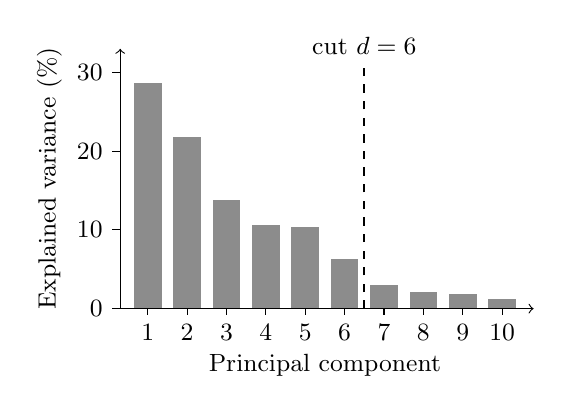
\begin{tikzpicture}[font=\small, x=0.5cm, y=0.1cm]
			% bars: share of the variance of every component in percent
			\foreach \i/\v in {1/28.67, 2/21.83, 3/13.85, 4/10.68, 5/10.43, 6/6.36, 7/3.04, 8/2.13, 9/1.82, 10/1.18}
				\fill[black!45] (\i - 0.35, 0) rectangle (\i + 0.35, \v);
			\draw[->] (0.3, 0) -- (10.8, 0);
			\draw[->] (0.3, 0) -- (0.3, 33);
			\foreach \i in {1, ..., 10}
				\draw (\i, 0) -- (\i, -0.8) node[below] {\i};
			\foreach \y in {0, 10, 20, 30}
				\draw (0.3, \y) -- (0.1, \y) node[left] {\y};
			\draw[dashed, thick] (6.5, 0) -- (6.5, 31) node[above] {cut $d = 6$};
			\node[below=0.45cm] at (5.5, 0) {Principal component};
			\node[rotate=90] at (-1.5, 16.5) {Explained variance (\%)};
		\end{tikzpicture}
		\caption{Explained variance per component}
		\label{fig:approach:pca_intra_variance}
	\end{subfigure}%
	\hfill
	\begin{subfigure}[b]{0.48\textwidth}
		\centering
		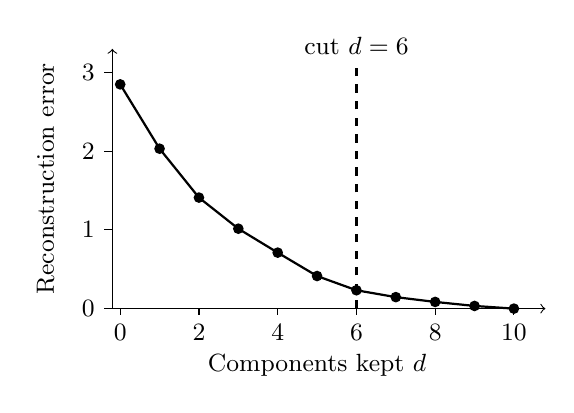
\begin{tikzpicture}[font=\small, x=0.5cm, y=1cm]
			\draw[->] (-0.2, 0) -- (10.8, 0);
			\draw[->] (-0.2, 0) -- (-0.2, 3.3);
			\foreach \d in {0, 2, ..., 10}
				\draw (\d, 0) -- (\d, -0.08) node[below] {\d};
			\foreach \y in {0, 1, 2, 3}
				\draw (-0.2, \y) -- (-0.4, \y) node[left] {\y};
			\draw[thick] plot[mark=*, mark size=1.5pt] coordinates {(0, 2.848) (1, 2.031) (2, 1.410) (3, 1.015) (4, 0.711) (5, 0.414) (6, 0.233) (7, 0.146) (8, 0.085) (9, 0.034) (10, 0)};
			\draw[dashed, thick] (6, 0) -- (6, 3.1) node[above] {cut $d = 6$};
			\node[below=0.45cm] at (5, 0) {Components kept $d$};
			\node[rotate=90] at (-1.9, 1.65) {Reconstruction error};
		\end{tikzpicture}
		\caption{Reconstruction error}
		\label{fig:approach:pca_intra_error}
	\end{subfigure}
	\caption[PCA of the intra-case features of the running example]{%
		PCA of the min-max normalized intra-case features of the running example $L_3$ (Example~\ref{ex:approach:reduction_intra}).
		\subref{fig:approach:pca_intra_variance}~Share of the variance that each principal component explains. Components 11 to 20 explain no variance.
		\subref{fig:approach:pca_intra_error}~Reconstruction error $\mathit{err}_{X'}(d)$ over the number $d$ of kept components. After the cut at $d = 6$ (dashed), a further component barely lowers the error.}
	\label{fig:approach:pca_intra}
\end{figure}

\begin{example}
	\label{ex:approach:reduction_intra}
	We normalize the 20 intra-case feature columns of $L_3$ (Example~\ref{ex:approach:intra}) except for the five binary columns of the current activity. Then, we fit the PCA on the 24,600 events (Figure~\ref{fig:approach:pca_intra}).
	\begin{itemize}
		\item The min-max normalization stretches, e.g., the frequencies of $d$ and $e$ from $[0, 0.25]$ to $[0, 1]$.

		\item The 24,600 rows only take 13 different vectors, one per prefix, and the columns are linearly dependent. Thus, only ten of the 20 principal components explain variance.

		\item The reconstruction error knee is reached after six components, which keep 91.8\% of the variance. Thus, we cut at $d = 6$.

		\item The first component mainly weights the directly-follows counts $b \to c$ and $a \to b$, the second $a \to c$ and $c \to b$. Thus, the first two principal components already separate the orders before and after the control-flow drift.
	\end{itemize}
\end{example}

\subsection{Resource Perspective}
\label{sec:approach:reduction:resource}
The resource feature matrix has a row per feature window and is therefore short. Its columns mix counts and shares with very different value ranges. Moreover, many shares change together, e.g., when another resource takes over an activity, its share rises and that of the previous resource falls.

\begin{figure}[tb]
	\centering
	\begin{subfigure}[b]{0.48\textwidth}
		\centering
		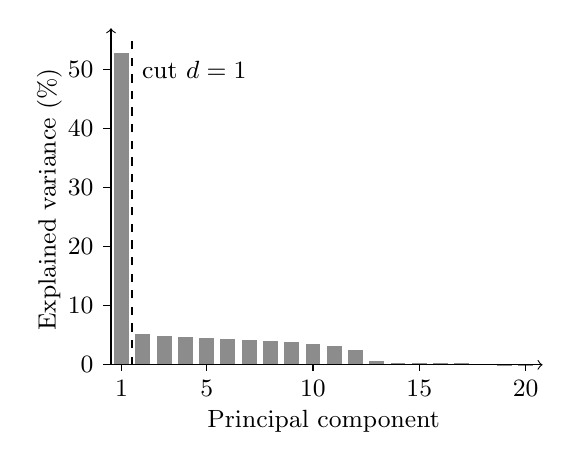
\begin{tikzpicture}[font=\small, x=0.27cm, y=0.075cm]
			% bars: share of the variance of every component in percent
			\foreach \i/\v in {1/52.88, 2/5.24, 3/4.84, 4/4.65, 5/4.48, 6/4.35, 7/4.28, 8/4.07, 9/3.88, 10/3.57, 11/3.23, 12/2.45, 13/0.70, 14/0.37, 15/0.33, 16/0.29, 17/0.28, 18/0.06, 19/0.03, 20/0.03}
				\fill[black!45] (\i - 0.35, 0) rectangle (\i + 0.35, \v);
			% share of the variance of a single standardized column
			\draw[->] (0.5, 0) -- (20.8, 0);
			\draw[->] (0.5, 0) -- (0.5, 57);
			\foreach \i in {1, 5, 10, 15, 20}
				\draw (\i, 0) -- (\i, -1.07) node[below] {\i};
			\foreach \y in {0, 10, ..., 50}
				\draw (0.5, \y) -- (0.13, \y) node[left] {\y};
			\draw[dashed, thick] (1.5, 0) -- (1.5, 55);
			\node[right] at (1.5, 50) {cut $d = 1$};
			\node[below=0.45cm] at (10.5, 0) {Principal component};
			\node[rotate=90] at (-2.4, 28) {Explained variance (\%)};
		\end{tikzpicture}
		\caption{Explained variance per component}
		\label{fig:approach:pca_resource_variance}
	\end{subfigure}%
	\hfill
	\begin{subfigure}[b]{0.48\textwidth}
		\centering
		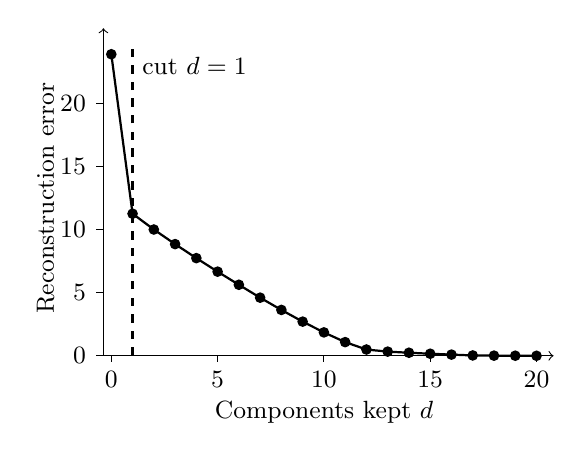
\begin{tikzpicture}[font=\small, x=0.27cm, y=0.16cm]
			\draw[->] (-0.37, 0) -- (20.8, 0);
			\draw[->] (-0.37, 0) -- (-0.37, 26);
			\foreach \d in {0, 5, ..., 20}
				\draw (\d, 0) -- (\d, -0.5) node[below] {\d};
			\foreach \y in {0, 5, ..., 20}
				\draw (-0.37, \y) -- (-0.74, \y) node[left] {\y};
			\draw[thick] plot[mark=*, mark size=1.5pt] coordinates {(0, 23.934) (1, 11.278) (2, 10.023) (3, 8.864) (4, 7.751) (5, 6.678) (6, 5.637) (7, 4.613) (8, 3.640) (9, 2.712) (10, 1.857) (11, 1.085) (12, 0.498) (13, 0.331) (14, 0.242) (15, 0.163) (16, 0.094) (17, 0.028) (18, 0.013) (19, 0.006) (20, 0)};
			\draw[dashed, thick] (1, 0) -- (1, 25);
			\node[right] at (1, 23) {cut $d = 1$};
			\node[below=0.45cm] at (10, 0) {Components kept $d$};
			\node[rotate=90] at (-3.1, 12.5) {Reconstruction error};
		\end{tikzpicture}
		\caption{Reconstruction error}
		\label{fig:approach:pca_resource_error}
	\end{subfigure}
	\caption[PCA of the resource features of the running example]{%
		PCA of the z-score standardized resource features of the running example $L_3$ (Example~\ref{ex:approach:reduction_resource}).
		\subref{fig:approach:pca_resource_variance}~Share of the variance that each principal component explains. \subref{fig:approach:pca_resource_error}~Reconstruction error $\mathit{err}_{X'}(d)$ over the number $d$ of kept components.}
	\label{fig:approach:pca_resource}
\end{figure}

\begin{example}
	\label{ex:approach:reduction_resource}
	We choose the z-score standardization, so that each of the 24 resource feature columns of $L_3$ (Example~\ref{ex:approach:resource}) contributes the same variance to the PCA. Then, we fit the PCA on the 366 feature windows (Figure~\ref{fig:approach:pca_resource}).
	\begin{itemize}
		\item Without scaling, the events per resource with standard deviations of up to 17.75 would dominate the shares with at most 0.41. The first component would then explain 83.8\% of the variance and weight almost only the events per resource.

		\item After the standardization, the first component explains 52.9\% of the variance. It weights the ten shares of the dominant resources before and after the reassignment with about $\pm 0.27$. The weights are negative for the dominant resources before the drift and positive for those after it, e.g., $-0.27$ for $a$ by \texttt{res\_01} and $+0.27$ for $a$ by \texttt{res\_03} (Table~\ref{tab:approach:features_resource}).

		\item The reconstruction error with the first component is 11.28 and we keep only the first component.

		\item The first component alone separates the feature windows before and after the drift. It lies between $-4.36$ and $-2.63$ for the 182 days before July~1 and between 1.95 and 4.56 for the 183 days after it.
	\end{itemize}
\end{example}

\subsection{Inter-Case Perspective}
\label{sec:approach:reduction:inter}
Most inter-case feature groups have a single column, so the inter-case feature matrix has only a few columns. These columns measure different quantities, e.g., counts, minutes and euros. Thus, scaling is essential, whereas PCA only saves a few dimensions. Without PCA, each dimension of $Z$ remains a named feature.

\begin{example}
	\label{ex:approach:reduction_inter}
	The inter-case feature matrix of $L_3$ has four columns and 731 feature windows (Example~\ref{ex:approach:inter}). We choose the z-score standardization and skip PCA, so the reduced matrix consists of the four standardized features.
	\begin{itemize}
		\item Without scaling, the mean amount with a standard deviation of 674 euros would explain 99.99\% of the variance, and the other three features would hardly count.

		\item The feature window of July~18, 00:00, contains no events, so all its features are 0. With the min-max normalization, this window would squeeze more than 90\% of the mean within-case gaps into $[0.73, 0.89]$. The z-score standardization gives all four features the standard deviation 1, and this window becomes an outlier with the standardized mean gap $-14.53$.

		\item The active cases and the new arrivals have the correlation 0.90. PCA merges them into the first component with 47.6\% of the variance, which gives the mean amount almost no weight. A cut at $d = 1$ would therefore lose the drift.

		\item The mean amount and the mean within-case gap are hardly correlated (0.07), so the second and third components mix them with almost equal weights. A cut at the elbow $d = 3$ would keep 97.4\% of the variance, but spread the amount over two components and only save one dimension.

		\item Without PCA, the standardized mean amount rises directly from $-0.67$ in the feature window of September~30, 00:00, to $1.48$ in that of October~1, 00:00 (Table~\ref{tab:approach:features_inter}).
	\end{itemize}
\end{example}

The three examples show that the explained variance alone does not decide the cut. The first resource component keeps only 52.9\% of the variance, but separates the days before and after the reassignment. The first inter-case component keeps almost as much, 47.6\%, but misses the amount drift.

\section{Clustering into States}
\label{sec:approach:clustering}
A clustering groups the rows (feature windows or events) of the reduced matrix such that rows that describe similar behavior end up in the same cluster. We treat each cluster as a state. We use the three clustering algorithms k-means, SOM and DBSCAN (Section~\ref{sec:prelim:clustering}). Similar to the previous steps, our framework is flexible and can easily be extended with further clustering algorithms such as k-medoids or hierarchical clustering. For each perspective, users choose the algorithm and its hyperparameters depending on the event log, e.g., in the dashboard (Section~\ref{sec:impl:dashboard}).

The algorithms also help to choose each other's hyperparameters. For example, a SOM with a large grid shows how many groups of frequently used cells lie far apart from each other, which suggests the number $k$ of clusters for k-means. The evaluation measures of Section~\ref{sec:prelim:cluster_eval} additionally show how good a clustering is and support the choice of the grid size, $k$, $\varepsilon$ and $\mathit{minPts}$.

Our framework supports various distances for the clustering. Besides the Euclidean distance, the SOM and DBSCAN also work with the Manhattan, Chebyshev and cosine distances (Section~\ref{sec:prelim:pca}). k-means only uses the Euclidean distance, since each of its centers is the mean of its vectors (Definition~\ref{def:prelim:kmeans}). In the running example, all three algorithms use the Euclidean distance.

\begin{definition}[States and Trajectories]
	\label{def:approach:states}
	Let $L$ be an event log, let $Z \in \R^{m \times d}$ be its reduced matrix with the rows $\mathbf{z}_1^\top, \dots, \mathbf{z}_m^\top$ (Definition~\ref{def:approach:reduction}), and let $\mathit{cl} \in \Set{1, \dots, m} \to K$ be a clustering of $Z$ by a SOM, k-means or DBSCAN (Definitions~\ref{def:prelim:som}, \ref{def:prelim:kmeans} and~\ref{def:prelim:dbscan}).
	\begin{itemize}
		\item $K$ is the set of states, and $\mathit{state}(\mathbf{z}_j) = \mathit{cl}(j)$ is the state of the row $\mathbf{z}_j$ for $1 \le j \le m$. For DBSCAN, $\mathit{noise}$ is also a state.
		\item In the intra-case perspective, each row belongs to an event (Definition~\ref{def:approach:feature_extraction}). A case whose events belong to the rows $\mathbf{z}_{j_1}, \dots, \mathbf{z}_{j_l}$ in the order $\preceq$ has the trajectory $\seq{\mathit{state}(\mathbf{z}_{j_1}), \dots, \mathit{state}(\mathbf{z}_{j_l})}$.
		\item In the resource and inter-case perspectives, the rows $\mathbf{z}_1, \dots, \mathbf{z}_m$ belong to the feature windows $W_L = \seq{w_1, \dots, w_m}$ (Definition~\ref{def:approach:windows}). The event log has the trajectory $\seq{\mathit{state}(\mathbf{z}_1), \dots, \mathit{state}(\mathbf{z}_m)}$.
	\end{itemize}
\end{definition}

\noindent\emph{Properties:}
\begin{itemize}[beginpenalty=10000]
	\item Similar to PCA, the clustering uses all rows of $Z$. Therefore, all process versions share the same states. A drift does not change the states, but how often each state occurs. Section~\ref{sec:approach:drift_signals} measures this change.
	\item In the intra-case perspective, each event has a state, whereas in the resource and inter-case perspectives each feature window has a state.
	\item Consecutive equal states of a trajectory form a visit of the state. A trajectory thus shows how long a case or the event log stays in a state.
	\item In the intra-case perspective, a trajectory only covers a single case. Thus, a drift only shows when we compare the trajectories of cases before and after it. In the resource and inter-case perspectives, the trajectory covers the whole event log, so a change of its state already indicates a drift.
	\item Each state has a representative vector: the prototype of its cell, its center or the mean of its core points. The distance between two representatives shows how similar two states are. Our implementation gives close states similar colors (Section~\ref{sec:impl:kairo}).
\end{itemize}

In each perspective of the running example, we use a different algorithm. Table~\ref{tab:approach:cluster_eval} shows the chosen clusterings, and the following examples interpret the resulting states.

\begin{table}[tb]
	\centering
	\caption[Evaluation of the chosen clusterings of the running example]{%
		Metrics of the chosen clusterings of $L_3$ (Section~\ref{sec:prelim:cluster_eval}). DBSCAN has two clusters and noise.}
	\label{tab:approach:cluster_eval}
	\small
	\begin{tabular}{@{}llrrrrrr@{}}
		\toprule
		Perspective & Clustering                                            & States & $\mathit{sil}$ & $\mathit{ch}$ & $\mathit{qe}$ & $\mathit{ent}$ & $\mathit{dbcv}$ \\
		\midrule
		Intra-case  & SOM, $3 \times 3$                                     & 9      & 0.857          & 36,694        & 0.288         & 0.973          & --              \\
		Resource    & k-means, $k = 2$                                      & 2      & 0.934          & 24,779        & --            & --             & --              \\
		Inter-case  & DBSCAN, $\varepsilon = 0.7$, $\mathit{minPts} = 8$    & 3      & 0.382          & 271           & --            & --             & 0.141           \\
		\bottomrule
	\end{tabular}
\end{table}

\subsection{Intra-Case Perspective}
\label{sec:approach:clustering:intra}
An intra-case state describes how far a case has progressed and on which path. Since the intra-case features only read the activities of a case, all cases of the same trace variant have the same trajectory. Thus, many events share the same row of the reduced matrix, e.g., the $k$-th events of all cases of a trace variant.

\begin{figure}[tb]
	\centering
	\definecolor{lineA}{RGB}{0,114,178}
	\definecolor{lineB}{RGB}{230,159,0}
	\begin{subfigure}[b]{0.48\textwidth}
		\centering
		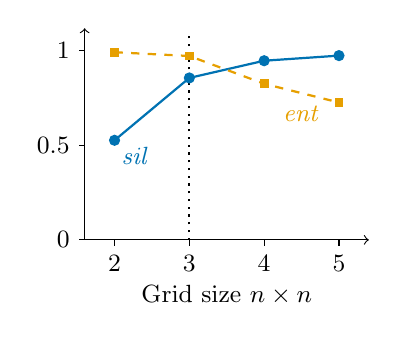
\begin{tikzpicture}[font=\small, x=0.95cm, y=2.4cm]
			\draw[->] (1.6, 0) -- (5.4, 0);
			\draw[->] (1.6, 0) -- (1.6, 1.12);
			\foreach \n in {2, ..., 5}
				\draw (\n, 0) -- (\n, -0.03) node[below] {$\n$};
			\foreach \y in {0, 0.5, 1}
				\draw (1.6, \y) -- (1.53, \y) node[left] {$\y$};
			\draw[dotted, thick] (3, 0) -- (3, 1.08);
			\draw[thick, lineA] plot[mark=*, mark size=1.6pt] coordinates {(2, 0.527) (3, 0.857) (4, 0.948) (5, 0.975)};
			\draw[thick, dashed, lineB] plot coordinates {(2, 0.993) (3, 0.973) (4, 0.826) (5, 0.727)};
			\foreach \n/\y in {2/0.993, 3/0.973, 4/0.826, 5/0.727}
				\fill[lineB] (\n, \y) ++(-1.6pt, -1.6pt) rectangle ++(3.2pt, 3.2pt);
			\node[lineA, below right=-1pt] at (2, 0.527) {$\mathit{sil}$};
			\node[lineB, below=1pt] at (4.5, 0.776) {$\mathit{ent}$};
			\node[below=0.45cm] at (3.5, 0) {Grid size $n \times n$};
		\end{tikzpicture}
		\caption{SOM evaluation}
		\label{fig:approach:cluster_eval_som}
	\end{subfigure}%
	\hfill
	\begin{subfigure}[b]{0.48\textwidth}
		\centering
		% generated by notebooks/thesis, do not edit by hand
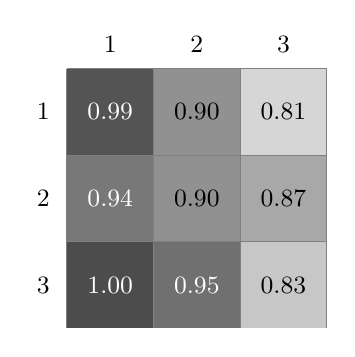
\begin{tikzpicture}[font=\small]
	\node at (-0.3, -0.550) {1};
	\fill[black!67] (0.000, 0.000) rectangle ++(1.10, -1.10);
	\node[text=white] at (0.550, -0.550) {0.99};
	\fill[black!43] (1.100, 0.000) rectangle ++(1.10, -1.10);
	\node[text=black] at (1.650, -0.550) {0.90};
	\fill[black!16] (2.200, 0.000) rectangle ++(1.10, -1.10);
	\node[text=black] at (2.750, -0.550) {0.81};
	\node at (-0.3, -1.650) {2};
	\fill[black!53] (0.000, -1.100) rectangle ++(1.10, -1.10);
	\node[text=white] at (0.550, -1.650) {0.94};
	\fill[black!43] (1.100, -1.100) rectangle ++(1.10, -1.10);
	\node[text=black] at (1.650, -1.650) {0.90};
	\fill[black!34] (2.200, -1.100) rectangle ++(1.10, -1.10);
	\node[text=black] at (2.750, -1.650) {0.87};
	\node at (-0.3, -2.750) {3};
	\fill[black!70] (0.000, -2.200) rectangle ++(1.10, -1.10);
	\node[text=white] at (0.550, -2.750) {1.00};
	\fill[black!56] (1.100, -2.200) rectangle ++(1.10, -1.10);
	\node[text=white] at (1.650, -2.750) {0.95};
	\fill[black!22] (2.200, -2.200) rectangle ++(1.10, -1.10);
	\node[text=black] at (2.750, -2.750) {0.83};
	\node at (0.550, 0.3) {1};
	\node at (1.650, 0.3) {2};
	\node at (2.750, 0.3) {3};
	\draw[black!50] (0, 0) grid[step=1.10] (3.300, -3.300);
\end{tikzpicture}

		\caption{U-matrix}
		\label{fig:approach:state_plots_umatrix}
	\end{subfigure}

	\medskip
	\begin{subfigure}{\textwidth}
		\centering
		% generated by notebooks/thesis, do not edit by hand
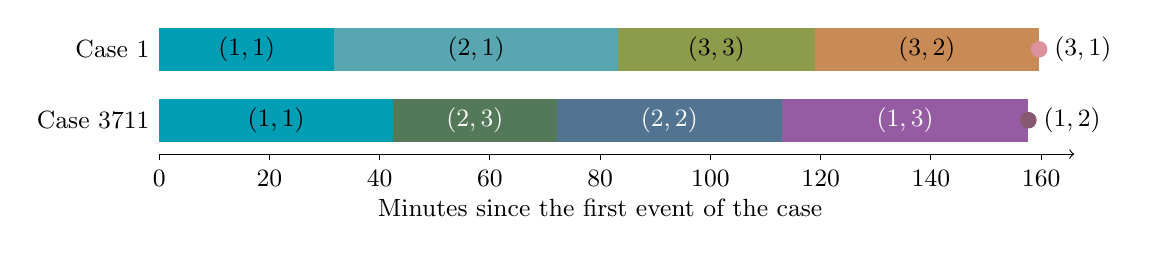
\begin{tikzpicture}[font=\small, x=0.07cm, y=1cm]
	\definecolor{trajectory0}{HTML}{009EB4}
	\definecolor{trajectory1}{HTML}{58A7B0}
	\definecolor{trajectory2}{HTML}{8D9C4A}
	\definecolor{trajectory3}{HTML}{C98B55}
	\definecolor{trajectory4}{HTML}{DB929C}
	\definecolor{trajectory5}{HTML}{547959}
	\definecolor{trajectory6}{HTML}{527491}
	\definecolor{trajectory7}{HTML}{955CA3}
	\definecolor{trajectory8}{HTML}{855A6E}
	\node[left] at (0, 0.28) {Case 1};
	\fill[trajectory0] (0.00, -0.00) rectangle (31.75, 0.55);
	\node[text=black] at (15.88, 0.28) {$(1, 1)$};
	\fill[trajectory1] (31.75, -0.00) rectangle (83.23, 0.55);
	\node[text=black] at (57.49, 0.28) {$(2, 1)$};
	\fill[trajectory2] (83.23, -0.00) rectangle (118.92, 0.55);
	\node[text=black] at (101.08, 0.28) {$(3, 3)$};
	\fill[trajectory3] (118.92, -0.00) rectangle (159.63, 0.55);
	\node[text=black] at (139.28, 0.28) {$(3, 2)$};
	\fill[trajectory4] (159.63, 0.28) circle (3pt) node[right=2pt, text=black] {$(3, 1)$};
	\node[left] at (0, -0.62) {Case 3711};
	\fill[trajectory0] (0.00, -0.90) rectangle (42.42, -0.35);
	\node[text=black] at (21.21, -0.62) {$(1, 1)$};
	\fill[trajectory5] (42.42, -0.90) rectangle (72.13, -0.35);
	\node[text=white] at (57.28, -0.62) {$(2, 3)$};
	\fill[trajectory6] (72.13, -0.90) rectangle (112.95, -0.35);
	\node[text=white] at (92.54, -0.62) {$(2, 2)$};
	\fill[trajectory7] (112.95, -0.90) rectangle (157.68, -0.35);
	\node[text=white] at (135.32, -0.62) {$(1, 3)$};
	\fill[trajectory8] (157.68, -0.62) circle (3pt) node[right=2pt, text=black] {$(1, 2)$};
	\draw[->] (0, -1.05) -- (166.00, -1.05);
	\draw (0, -1.05) -- (0, -1.13) node[below] {0};
	\draw (20, -1.05) -- (20, -1.13) node[below] {20};
	\draw (40, -1.05) -- (40, -1.13) node[below] {40};
	\draw (60, -1.05) -- (60, -1.13) node[below] {60};
	\draw (80, -1.05) -- (80, -1.13) node[below] {80};
	\draw (100, -1.05) -- (100, -1.13) node[below] {100};
	\draw (120, -1.05) -- (120, -1.13) node[below] {120};
	\draw (140, -1.05) -- (140, -1.13) node[below] {140};
	\draw (160, -1.05) -- (160, -1.13) node[below] {160};
	\node[below=0.45cm] at (80.0, -1.05) {Minutes since the first event of the case};
\end{tikzpicture}

		\caption{Trajectories of case~1 and case~3711}
		\label{fig:approach:trajectories_cases}
	\end{subfigure}
	\caption[Intra-case clustering of the running example]{%
		SOM clustering of the intra-case features of the running example $L_3$ (Example~\ref{ex:approach:clustering_intra}).
		\subref{fig:approach:cluster_eval_som}~Silhouette (blue) and occupancy entropy (orange) over the grid size. The dotted line marks the chosen $3 \times 3$ grid.
		\subref{fig:approach:state_plots_umatrix}~Mean distance of the prototype of each cell to the prototypes of its neighboring cells, divided by the largest mean.
		\subref{fig:approach:trajectories_cases}~Each box is a visit of a state with its cell of Figure~\ref{fig:approach:som_intra}. The last state of a case is a dot.}
	\label{fig:approach:clustering_intra}
\end{figure}

\begin{figure}[tb]
	\centering
	\definecolor{stateFill}{RGB}{0,114,178}
	\definecolor{trajectory}{RGB}{213,94,0}
	\tikzset{
		cell/.style={draw=black!50},
		prefixes/.style={font=\small\itshape, align=center, anchor=north, inner sep=0pt},
		visit/.style={circle, fill=trajectory, text=white, font=\small\bfseries, inner sep=1pt, minimum size=4mm},
	}
	% square cells of 1.4 cm: #1 row, #2 column, #3 fill intensity, #4 prefixes, one per line,
	% #5 position of the cell in the trajectory
	\newcommand*{\somcell}[5]{%
		\fill[stateFill!#3] ({(#2 - 1) * 1.4}, {-(#1 - 1) * 1.4}) rectangle ++(1.4, -1.4);
		\draw[cell] ({(#2 - 1) * 1.4}, {-(#1 - 1) * 1.4}) rectangle ++(1.4, -1.4);
		\node[prefixes] at ({(#2 - 0.5) * 1.4}, {-(#1 - 1) * 1.4 - 0.12}) {#4};
		\if\relax\detokenize{#5}\relax\else
			\node[visit] at ({(#2 - 0.5) * 1.4}, {-#1 * 1.4 + 0.29}) {#5};
		\fi
	}
	\newcommand*{\gridlabels}{%
		\foreach \k in {1, 2, 3} {
			\node[font=\small] at ({(\k - 0.5) * 1.4}, 0.3) {$\k$};
			\node[font=\small] at (-0.3, {-(\k - 0.5) * 1.4}) {$\k$};
		}
	}
	\begin{subfigure}[t]{0.49\textwidth}
		\centering
		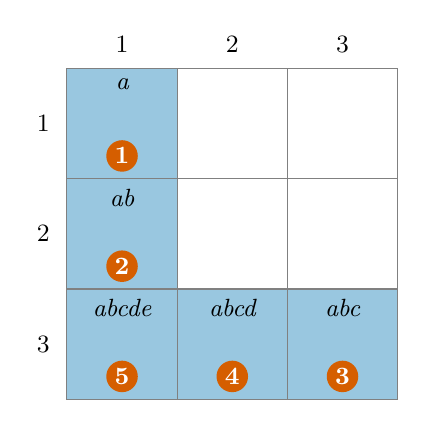
\begin{tikzpicture}
			\gridlabels
			\somcell{1}{1}{40}{a}{1}
			\somcell{1}{2}{0}{}{}
			\somcell{1}{3}{0}{}{}
			\somcell{2}{1}{40}{ab}{2}
			\somcell{2}{2}{0}{}{}
			\somcell{2}{3}{0}{}{}
			\somcell{3}{1}{40}{abcde}{5}
			\somcell{3}{2}{40}{abcd}{4}
			\somcell{3}{3}{40}{abc}{3}
		\end{tikzpicture}
		\caption{Before the drift, with case 1}
		\label{fig:approach:som_intra_before}
	\end{subfigure}%
	\hfill
	\begin{subfigure}[t]{0.49\textwidth}
		\centering
		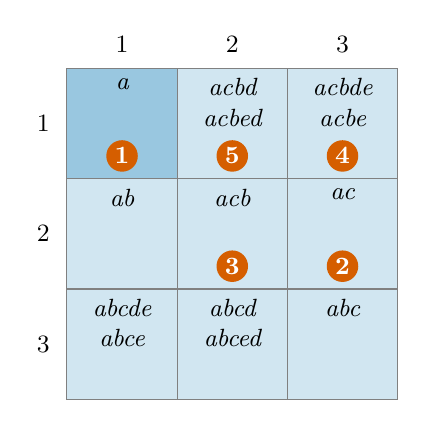
\begin{tikzpicture}
			\gridlabels
			\somcell{1}{1}{40}{a}{1}
			\somcell{1}{2}{18}{acbd\\acbed}{5}
			\somcell{1}{3}{18}{acbde\\acbe}{4}
			\somcell{2}{1}{18}{ab}{}
			\somcell{2}{2}{18}{acb}{3}
			\somcell{2}{3}{18}{ac}{2}
			\somcell{3}{1}{18}{abcde\\abce}{}
			\somcell{3}{2}{18}{abcd\\abced}{}
			\somcell{3}{3}{18}{abc}{}
		\end{tikzpicture}
		\caption{After the drift, with case 3711}
		\label{fig:approach:som_intra_after}
	\end{subfigure}
	\caption[Intra-case states of the running example]{%
		The $3 \times 3$ SOM of the intra-case states of $L_3$ (Example~\ref{ex:approach:clustering_intra}). Each cell lists the prefixes of its events, e.g., \emph{abc} for $\seq{a, b, c}$. Dark cells hold about 20\% and light cells about 10\% of the events. A circle with the number $k$ marks the state of the $k$-th event of the case.
		\subref{fig:approach:som_intra_before}~The 6,255 events before the drift fall into five cells.
		\subref{fig:approach:som_intra_after}~The 18,345 events after the drift use all nine cells.}
	\label{fig:approach:som_intra}
\end{figure}

\begin{example}
	\label{ex:approach:clustering_intra}
	Like \textcite{berti2025ocel}, we choose a SOM, interpret its cells as states and read the trajectory of a case as a path on the grid. Neighboring cells have similar prototypes, so the grid also shows which states are similar. We cluster the reduced intra-case matrix of $L_3$ (Example~\ref{ex:approach:reduction_intra}) with SOMs of the grid sizes $2 \times 2$ to $5 \times 5$ (Figure~\ref{fig:approach:cluster_eval_som}). With the grid size, the quantization error falls from 0.917 to 0.052, and the silhouette rises from 0.527 to 0.975. At the same time, the occupancy entropy falls from 0.993 to 0.727, since the $5 \times 5$ grid only uses 12 cells and gives almost each of the 13 prefixes its own cell. The $3 \times 3$ grid uses all cells almost evenly with the occupancy entropy 0.973 and reaches the silhouette 0.857 with the quantization error 0.288. Thus, we choose the $3 \times 3$ grid (Figure~\ref{fig:approach:som_intra}).
	\begin{itemize}
		\item Before the control-flow drift, all cases follow the trace $\seq{a, b, c, d, e}$. Its five prefixes occupy five cells, and case~1 has the trajectory $\seq{(1, 1),\allowbreak (2, 1),\allowbreak (3, 3),\allowbreak (3, 2),\allowbreak (3, 1)}$.

		\item After the drift, the prefixes that start with $\seq{a, c}$ occupy the four remaining cells. Case~3711 has the trajectory $\seq{(1, 1),\allowbreak (2, 3),\allowbreak (2, 2),\allowbreak (1, 3),\allowbreak (1, 2)}$ and thus only shares its first state with case~1.

		\item The prefixes $\seq{a, b, c, e}$ and $\seq{a, b, c, e, d}$ only occur after the drift, but share their cells with older prefixes. Thus, the cells $(3, 1)$ and $(3, 2)$ occur before and after the drift.

		\item Both cases take about 160~minutes, and each of their first four visits lasts 30 to 51~minutes (Figure~\ref{fig:approach:trajectories_cases}). Thus, the drift changes the states, but not the duration of the cases.

		\item The prototypes of consecutive states of both cases lie 1.63 to 2.00 apart, and those of all states 2.23 on average. Since our implementation chooses the colors by these distances, the color only changes gradually along a trajectory.

		\item The U-matrix only ranges from 0.81 to 1.00, so the grid shows no border between larger groups of states (Figure~\ref{fig:approach:state_plots_umatrix}). The four new cells form the top right region. Their prototypes lie closer to their neighbors than those of the old cells, with 0.87 against 0.94 on average.
	\end{itemize}
\end{example}

\subsection{Resource Perspective}
\label{sec:approach:clustering:resource}
A resource state describes how the work of a feature window is distributed among the resources. Consecutive feature windows of a stable process lie close together, so a few compact clusters suffice.

\begin{figure}[tb]
	\centering
	\definecolor{stateA}{RGB}{0,114,178}
	\definecolor{stateB}{RGB}{230,159,0}
	\begin{subfigure}{\textwidth}
		\centering
		% generated by notebooks/thesis, do not edit by hand
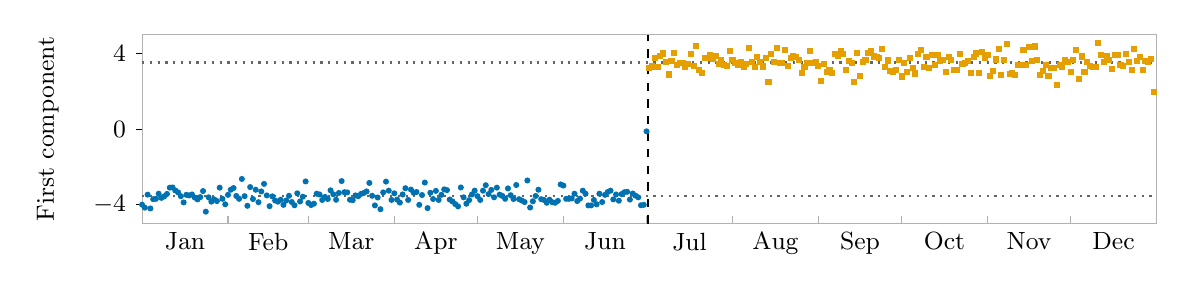
\begin{tikzpicture}[font=\small, x=0.0352cm, y=0.240cm]
	\draw[black!30] (0, -5.00) rectangle (366, 5.00);
	\node[below, inner sep=1pt] at (15.5, -5.30) {Jan};
	\node[below, inner sep=1pt] at (45.5, -5.30) {Feb};
	\draw[black!30] (31.0, -5.00) -- (31.0, -4.60);
	\node[below, inner sep=1pt] at (75.5, -5.30) {Mar};
	\draw[black!30] (60.0, -5.00) -- (60.0, -4.60);
	\node[below, inner sep=1pt] at (106.0, -5.30) {Apr};
	\draw[black!30] (91.0, -5.00) -- (91.0, -4.60);
	\node[below, inner sep=1pt] at (136.5, -5.30) {May};
	\draw[black!30] (121.0, -5.00) -- (121.0, -4.60);
	\node[below, inner sep=1pt] at (167.0, -5.30) {Jun};
	\draw[black!30] (152.0, -5.00) -- (152.0, -4.60);
	\node[below, inner sep=1pt] at (197.5, -5.30) {Jul};
	\draw[black!30] (182.0, -5.00) -- (182.0, -4.60);
	\node[below, inner sep=1pt] at (228.5, -5.30) {Aug};
	\draw[black!30] (213.0, -5.00) -- (213.0, -4.60);
	\node[below, inner sep=1pt] at (259.0, -5.30) {Sep};
	\draw[black!30] (244.0, -5.00) -- (244.0, -4.60);
	\node[below, inner sep=1pt] at (289.5, -5.30) {Oct};
	\draw[black!30] (274.0, -5.00) -- (274.0, -4.60);
	\node[below, inner sep=1pt] at (320.0, -5.30) {Nov};
	\draw[black!30] (305.0, -5.00) -- (305.0, -4.60);
	\node[below, inner sep=1pt] at (350.5, -5.30) {Dec};
	\draw[black!30] (335.0, -5.00) -- (335.0, -4.60);
	\draw (0, -4.00) -- ++(-0.08cm, 0) node[left] {$-4$};
	\draw (0, 0.00) -- ++(-0.08cm, 0) node[left] {$0$};
	\draw (0, 4.00) -- ++(-0.08cm, 0) node[left] {$4$};
	\node[rotate=90] at (-34, 0.00) {First component};
	\draw[dotted, thick, black!60] (0, -3.53) -- (366, -3.53);
	\draw[dotted, thick, black!60] (0, 3.53) -- (366, 3.53);
	\draw[dashed, thick] (182.50, -5.00) -- (182.50, 5.00);
	\foreach \x/\y in {0.00/-3.99, 1.00/-4.15, 2.00/-3.46, 3.00/-4.19, 4.00/-3.70, 5.00/-3.68, 6.00/-3.41, 7.00/-3.63, 8.00/-3.55, 9.00/-3.42, 10.00/-3.09, 11.00/-3.08, 12.00/-3.24, 13.00/-3.34, 14.00/-3.54, 15.00/-3.87, 16.00/-3.47, 17.00/-3.50, 18.00/-3.45, 19.00/-3.61, 20.00/-3.71, 21.00/-3.59, 22.00/-3.27, 23.00/-4.36, 24.00/-3.60, 25.00/-3.83, 26.00/-3.71, 27.00/-3.80, 28.00/-3.09, 29.00/-3.68, 30.00/-3.97, 31.00/-3.47, 32.00/-3.20, 33.00/-3.11, 34.00/-3.53, 35.00/-3.68, 36.00/-2.63, 37.00/-3.54, 38.00/-4.05, 39.00/-3.06, 40.00/-3.69, 41.00/-3.20, 42.00/-3.86, 43.00/-3.29, 44.00/-2.89, 45.00/-3.50, 46.00/-4.07, 47.00/-3.55, 48.00/-3.77, 49.00/-3.83, 50.00/-3.73, 51.00/-4.00, 52.00/-3.77, 53.00/-3.52, 54.00/-3.85, 55.00/-4.02, 56.00/-3.39, 57.00/-3.82, 58.00/-3.57, 59.00/-2.76, 60.00/-3.90, 61.00/-4.01, 62.00/-3.94, 63.00/-3.41, 64.00/-3.45, 65.00/-3.74, 66.00/-3.58, 67.00/-3.69, 68.00/-3.23, 69.00/-3.44, 70.00/-3.73, 71.00/-3.37, 72.00/-2.74, 73.00/-3.33, 74.00/-3.34, 75.00/-3.73, 76.00/-3.75, 77.00/-3.50, 78.00/-3.54, 79.00/-3.42, 80.00/-3.37, 81.00/-3.29, 82.00/-2.84, 83.00/-3.52, 84.00/-4.03, 85.00/-3.61, 86.00/-4.23, 87.00/-3.34, 88.00/-2.77, 89.00/-3.25, 90.00/-3.74, 91.00/-3.39, 92.00/-3.72, 93.00/-3.88, 94.00/-3.45, 95.00/-3.12, 96.00/-3.74, 97.00/-3.19, 98.00/-3.36, 99.00/-3.32, 100.00/-4.00, 101.00/-3.48, 102.00/-2.82, 103.00/-4.17, 104.00/-3.36, 105.00/-3.69, 106.00/-3.26, 107.00/-3.74, 108.00/-3.47, 109.00/-3.18, 110.00/-3.22, 111.00/-3.72, 112.00/-3.82, 113.00/-3.96, 114.00/-4.08, 115.00/-3.08, 116.00/-3.60, 117.00/-3.94, 118.00/-3.75, 119.00/-3.45, 120.00/-3.25, 121.00/-3.54, 122.00/-3.74, 123.00/-3.25, 124.00/-2.96, 125.00/-3.43, 126.00/-3.21, 127.00/-3.60, 128.00/-3.09, 129.00/-3.46, 130.00/-3.53, 131.00/-3.68, 132.00/-3.13, 133.00/-3.49, 134.00/-3.69, 135.00/-2.95, 136.00/-3.70, 137.00/-3.77, 138.00/-3.85, 139.00/-2.71, 140.00/-4.14, 141.00/-3.81, 142.00/-3.53, 143.00/-3.20, 144.00/-3.70, 145.00/-3.74, 146.00/-3.89, 147.00/-3.73, 148.00/-3.86, 149.00/-3.89, 150.00/-3.79, 151.00/-2.92, 152.00/-2.98, 153.00/-3.68, 154.00/-3.68, 155.00/-3.66, 156.00/-3.41, 157.00/-3.80, 158.00/-3.67, 159.00/-3.25, 160.00/-3.41, 161.00/-4.03, 162.00/-4.03, 163.00/-3.74, 164.00/-3.97, 165.00/-3.41, 166.00/-3.85, 167.00/-3.47, 168.00/-3.32, 169.00/-3.25, 170.00/-3.71, 171.00/-3.45, 172.00/-3.78, 173.00/-3.43, 174.00/-3.33, 175.00/-3.31, 176.00/-3.72, 177.00/-3.40, 178.00/-3.51, 179.00/-3.60, 180.00/-4.02, 181.00/-4.00, 182.00/-0.11} \fill[stateA] (\x, \y) circle (1.1pt);
	\foreach \x/\y in {183.00/3.23, 184.00/3.32, 185.00/3.77, 186.00/3.29, 187.00/3.87, 188.00/4.01, 189.00/3.54, 190.00/2.90, 191.00/3.62, 192.00/4.03, 193.00/3.41, 194.00/3.51, 195.00/3.51, 196.00/3.28, 197.00/3.43, 198.00/3.99, 199.00/3.37, 200.00/4.43, 201.00/3.12, 202.00/3.00, 203.00/3.75, 204.00/3.77, 205.00/3.91, 206.00/3.73, 207.00/3.89, 208.00/3.44, 209.00/3.68, 210.00/3.42, 211.00/3.34, 212.00/4.14, 213.00/3.68, 214.00/3.53, 215.00/3.40, 216.00/3.56, 217.00/3.32, 218.00/3.46, 219.00/4.29, 220.00/3.58, 221.00/3.31, 222.00/3.84, 223.00/3.58, 224.00/3.32, 225.00/3.77, 226.00/2.49, 227.00/3.97, 228.00/3.55, 229.00/4.29, 230.00/3.50, 231.00/3.50, 232.00/4.18, 233.00/3.35, 234.00/3.76, 235.00/3.89, 236.00/3.84, 237.00/3.66, 238.00/2.98, 239.00/3.29, 240.00/3.49, 241.00/4.12, 242.00/3.49, 243.00/3.58, 244.00/3.34, 245.00/2.55, 246.00/3.46, 247.00/3.05, 248.00/3.12, 249.00/2.99, 250.00/3.96, 251.00/3.88, 252.00/4.12, 253.00/3.99, 254.00/3.16, 255.00/3.63, 256.00/3.50, 257.00/2.49, 258.00/4.03, 259.00/2.81, 260.00/3.57, 261.00/3.65, 262.00/4.05, 263.00/4.16, 264.00/3.85, 265.00/3.80, 266.00/3.76, 267.00/4.26, 268.00/3.29, 269.00/3.64, 270.00/3.07, 271.00/3.03, 272.00/3.16, 273.00/3.66, 274.00/2.79, 275.00/3.51, 276.00/3.02, 277.00/3.78, 278.00/3.26, 279.00/2.95, 280.00/4.00, 281.00/4.21, 282.00/3.31, 283.00/3.80, 284.00/3.25, 285.00/3.91, 286.00/3.38, 287.00/3.92, 288.00/3.64, 289.00/3.68, 290.00/3.03, 291.00/3.82, 292.00/3.68, 293.00/3.14, 294.00/3.16, 295.00/4.00, 296.00/3.44, 297.00/3.51, 298.00/3.59, 299.00/2.98, 300.00/3.81, 301.00/4.01, 302.00/2.97, 303.00/4.09, 304.00/3.75, 305.00/3.94, 306.00/2.83, 307.00/3.07, 308.00/3.69, 309.00/4.25, 310.00/2.89, 311.00/3.66, 312.00/4.51, 313.00/2.93, 314.00/2.99, 315.00/2.85, 316.00/3.41, 317.00/3.40, 318.00/4.20, 319.00/3.39, 320.00/4.36, 321.00/3.62, 322.00/4.38, 323.00/3.66, 324.00/2.89, 325.00/3.08, 326.00/3.38, 327.00/2.82, 328.00/3.24, 329.00/3.24, 330.00/2.35, 331.00/3.42, 332.00/3.32, 333.00/3.66, 334.00/3.55, 335.00/3.05, 336.00/3.66, 337.00/4.18, 338.00/2.68, 339.00/3.85, 340.00/3.04, 341.00/3.56, 342.00/3.33, 343.00/3.30, 344.00/3.29, 345.00/4.56, 346.00/3.91, 347.00/3.58, 348.00/3.87, 349.00/3.66, 350.00/3.20, 351.00/3.91, 352.00/3.95, 353.00/3.42, 354.00/3.34, 355.00/3.97, 356.00/3.57, 357.00/3.14, 358.00/4.24, 359.00/3.60, 360.00/3.84, 361.00/3.16, 362.00/3.63, 363.00/3.56, 364.00/3.71, 365.00/1.95} \fill[stateB] (\x, \y) ++(-1.1pt, -1.1pt) rectangle ++(2.2pt, 2.2pt);
\end{tikzpicture}

		\caption{First principal component of the feature windows}
		\label{fig:approach:states_resource}
	\end{subfigure}

	\medskip
	\begin{subfigure}{\textwidth}
		\centering
		% generated by notebooks/thesis, do not edit by hand
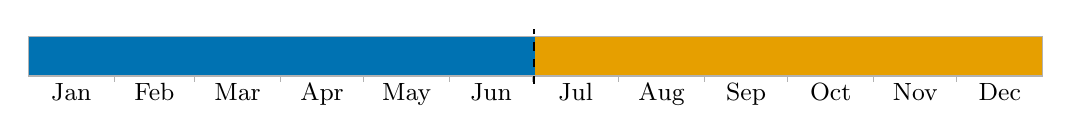
\begin{tikzpicture}[font=\small, x=0.0352cm, y=1cm]
	\fill[stateA] (0.00, 0) rectangle (183.00, 0.5);
	\fill[stateB] (183.00, 0) rectangle (366.00, 0.5);
	\draw[black!30] (0, 0) rectangle (366, 0.5);
	\draw[dashed, thick] (182.50, -0.1) -- (182.50, 0.6);
	\node[below, inner sep=1pt] at (15.5, -0.05) {Jan};
	\node[below, inner sep=1pt] at (45.5, -0.05) {Feb};
	\draw[black!30] (31.0, 0) -- (31.0, -0.08);
	\node[below, inner sep=1pt] at (75.5, -0.05) {Mar};
	\draw[black!30] (60.0, 0) -- (60.0, -0.08);
	\node[below, inner sep=1pt] at (106.0, -0.05) {Apr};
	\draw[black!30] (91.0, 0) -- (91.0, -0.08);
	\node[below, inner sep=1pt] at (136.5, -0.05) {May};
	\draw[black!30] (121.0, 0) -- (121.0, -0.08);
	\node[below, inner sep=1pt] at (167.0, -0.05) {Jun};
	\draw[black!30] (152.0, 0) -- (152.0, -0.08);
	\node[below, inner sep=1pt] at (197.5, -0.05) {Jul};
	\draw[black!30] (182.0, 0) -- (182.0, -0.08);
	\node[below, inner sep=1pt] at (228.5, -0.05) {Aug};
	\draw[black!30] (213.0, 0) -- (213.0, -0.08);
	\node[below, inner sep=1pt] at (259.0, -0.05) {Sep};
	\draw[black!30] (244.0, 0) -- (244.0, -0.08);
	\node[below, inner sep=1pt] at (289.5, -0.05) {Oct};
	\draw[black!30] (274.0, 0) -- (274.0, -0.08);
	\node[below, inner sep=1pt] at (320.0, -0.05) {Nov};
	\draw[black!30] (305.0, 0) -- (305.0, -0.08);
	\node[below, inner sep=1pt] at (350.5, -0.05) {Dec};
	\draw[black!30] (335.0, 0) -- (335.0, -0.08);
\end{tikzpicture}

		\caption{Trajectory of the event log}
		\label{fig:approach:trajectories_resource}
	\end{subfigure}
	\caption[Resource clustering of the running example]{%
		k-means clustering of the resource features of the running example $L_3$ (Example~\ref{ex:approach:clustering_resource}). Blue is state~1 and orange state~2.
		\subref{fig:approach:states_resource}~Each symbol is a feature window. The dotted lines are the two centers.
		\subref{fig:approach:trajectories_resource}~Each box is a visit of a state.
		Dashed lines mark the reassignment drift.}
	\label{fig:approach:clustering_resource}
\end{figure}

\begin{example}
	\label{ex:approach:clustering_resource}
	Since a few compact clusters suffice, we choose k-means with a small $k$. The reduced resource matrix of $L_3$ only has the first principal component (Example~\ref{ex:approach:reduction_resource}). For $k = 2$, k-means reaches the highest silhouette of 0.934 and the highest Cali\'nski--Harabasz index of 24,779. For $k = 3$ to 5, the silhouette drops to between 0.719 and 0.739, and for $k = 6$ to 0.539. Thus, we choose $k = 2$ with the centers $-3.53$ and $3.53$ (Figure~\ref{fig:approach:states_resource}).
	\begin{itemize}
		\item State~1 contains the 183 days up to July~1, and state~2 the 183 days from July~2. Thus, the trajectory of the event log consists of two visits of 183 days each (Figure~\ref{fig:approach:trajectories_resource}).

		\item The feature window of July~1 contains the reassignment at 12:00. With $-0.11$, the feature window lies between both centers, but since k-means assigns each row to a state, it is assigned to state~1.

		\item With $k = 3$, k-means splits the days after the drift into two states, and the trajectory has 96 instead of two visits. With $k = 6$, it also splits the days before the drift. These state changes look like drifts, although the process is stable.
	\end{itemize}
\end{example}

\subsection{Inter-Case Perspective}
\label{sec:approach:clustering:inter}
An inter-case state describes the load and the cases of a feature window. Unusual feature windows, e.g., with very few arrivals, occur in every process version, but do not describe a typical situation of the process.

\begin{figure}[tbp]
	\centering
	\definecolor{stateA}{RGB}{0,114,178}
	\definecolor{stateB}{RGB}{230,159,0}
	\begin{subfigure}[b]{0.42\textwidth}
		\centering
		% generated by notebooks/thesis, do not edit by hand
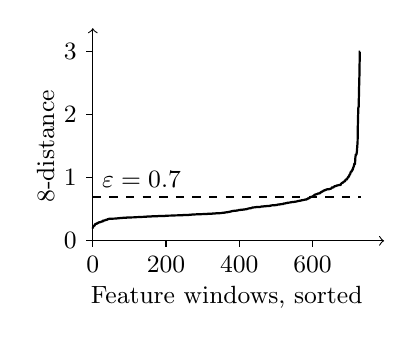
\begin{tikzpicture}[font=\small]
	\draw[->] (0, 0) -- (3.70, 0);
	\draw[->] (0, 0) -- (0, 2.70);
	\draw[thick] plot coordinates {(0.000, 0.157) (0.005, 0.182) (0.009, 0.187) (0.014, 0.190) (0.019, 0.194) (0.023, 0.195) (0.028, 0.209) (0.033, 0.214) (0.037, 0.215) (0.042, 0.215) (0.047, 0.219) (0.051, 0.220) (0.056, 0.220) (0.060, 0.227) (0.065, 0.227) (0.070, 0.228) (0.074, 0.231) (0.079, 0.235) (0.084, 0.237) (0.088, 0.237) (0.093, 0.237) (0.098, 0.238) (0.102, 0.240) (0.107, 0.242) (0.112, 0.245) (0.116, 0.245) (0.121, 0.246) (0.126, 0.247) (0.130, 0.255) (0.135, 0.256) (0.140, 0.257) (0.144, 0.258) (0.149, 0.258) (0.153, 0.260) (0.158, 0.263) (0.163, 0.265) (0.167, 0.265) (0.172, 0.268) (0.177, 0.269) (0.181, 0.269) (0.186, 0.272) (0.191, 0.275) (0.195, 0.275) (0.200, 0.277) (0.205, 0.277) (0.209, 0.280) (0.214, 0.281) (0.219, 0.281) (0.223, 0.281) (0.228, 0.281) (0.233, 0.281) (0.237, 0.281) (0.242, 0.281) (0.247, 0.281) (0.251, 0.281) (0.256, 0.281) (0.260, 0.282) (0.265, 0.282) (0.270, 0.282) (0.274, 0.282) (0.279, 0.282) (0.284, 0.283) (0.288, 0.283) (0.293, 0.283) (0.298, 0.283) (0.302, 0.284) (0.307, 0.285) (0.312, 0.285) (0.316, 0.286) (0.321, 0.286) (0.326, 0.287) (0.330, 0.287) (0.335, 0.287) (0.340, 0.288) (0.344, 0.289) (0.349, 0.289) (0.353, 0.289) (0.358, 0.289) (0.363, 0.290) (0.367, 0.290) (0.372, 0.291) (0.377, 0.291) (0.381, 0.292) (0.386, 0.292) (0.391, 0.292) (0.395, 0.292) (0.400, 0.293) (0.405, 0.293) (0.409, 0.293) (0.414, 0.294) (0.419, 0.294) (0.423, 0.294) (0.428, 0.294) (0.433, 0.296) (0.437, 0.296) (0.442, 0.296) (0.447, 0.296) (0.451, 0.296) (0.456, 0.296) (0.460, 0.296) (0.465, 0.296) (0.470, 0.297) (0.474, 0.297) (0.479, 0.297) (0.484, 0.297) (0.488, 0.297) (0.493, 0.297) (0.498, 0.298) (0.502, 0.298) (0.507, 0.298) (0.512, 0.298) (0.516, 0.298) (0.521, 0.298) (0.526, 0.299) (0.530, 0.299) (0.535, 0.300) (0.540, 0.300) (0.544, 0.300) (0.549, 0.300) (0.553, 0.300) (0.558, 0.301) (0.563, 0.301) (0.567, 0.301) (0.572, 0.301) (0.577, 0.302) (0.581, 0.302) (0.586, 0.303) (0.591, 0.303) (0.595, 0.303) (0.600, 0.303) (0.605, 0.303) (0.609, 0.303) (0.614, 0.303) (0.619, 0.303) (0.623, 0.303) (0.628, 0.304) (0.633, 0.304) (0.637, 0.304) (0.642, 0.304) (0.647, 0.305) (0.651, 0.305) (0.656, 0.306) (0.660, 0.306) (0.665, 0.306) (0.670, 0.306) (0.674, 0.307) (0.679, 0.307) (0.684, 0.307) (0.688, 0.308) (0.693, 0.309) (0.698, 0.309) (0.702, 0.309) (0.707, 0.309) (0.712, 0.310) (0.716, 0.310) (0.721, 0.310) (0.726, 0.310) (0.730, 0.310) (0.735, 0.310) (0.740, 0.310) (0.744, 0.310) (0.749, 0.311) (0.753, 0.311) (0.758, 0.311) (0.763, 0.311) (0.767, 0.311) (0.772, 0.311) (0.777, 0.311) (0.781, 0.311) (0.786, 0.312) (0.791, 0.312) (0.795, 0.313) (0.800, 0.313) (0.805, 0.313) (0.809, 0.313) (0.814, 0.313) (0.819, 0.313) (0.823, 0.313) (0.828, 0.314) (0.833, 0.314) (0.837, 0.314) (0.842, 0.314) (0.847, 0.314) (0.851, 0.314) (0.856, 0.314) (0.860, 0.314) (0.865, 0.315) (0.870, 0.315) (0.874, 0.315) (0.879, 0.315) (0.884, 0.315) (0.888, 0.315) (0.893, 0.315) (0.898, 0.315) (0.902, 0.315) (0.907, 0.316) (0.912, 0.316) (0.916, 0.316) (0.921, 0.317) (0.926, 0.318) (0.930, 0.318) (0.935, 0.318) (0.940, 0.318) (0.944, 0.318) (0.949, 0.318) (0.953, 0.319) (0.958, 0.319) (0.963, 0.320) (0.967, 0.320) (0.972, 0.320) (0.977, 0.320) (0.981, 0.320) (0.986, 0.320) (0.991, 0.320) (0.995, 0.321) (1.000, 0.321) (1.005, 0.321) (1.009, 0.321) (1.014, 0.321) (1.019, 0.322) (1.023, 0.322) (1.028, 0.322) (1.033, 0.322) (1.037, 0.322) (1.042, 0.322) (1.047, 0.323) (1.051, 0.323) (1.056, 0.323) (1.060, 0.323) (1.065, 0.323) (1.070, 0.323) (1.074, 0.323) (1.079, 0.324) (1.084, 0.324) (1.088, 0.324) (1.093, 0.324) (1.098, 0.324) (1.102, 0.324) (1.107, 0.325) (1.112, 0.325) (1.116, 0.325) (1.121, 0.325) (1.126, 0.325) (1.130, 0.325) (1.135, 0.325) (1.140, 0.325) (1.144, 0.327) (1.149, 0.327) (1.153, 0.327) (1.158, 0.327) (1.163, 0.327) (1.167, 0.327) (1.172, 0.328) (1.177, 0.328) (1.181, 0.328) (1.186, 0.328) (1.191, 0.328) (1.195, 0.329) (1.200, 0.329) (1.205, 0.329) (1.209, 0.329) (1.214, 0.329) (1.219, 0.329) (1.223, 0.330) (1.228, 0.330) (1.233, 0.331) (1.237, 0.331) (1.242, 0.332) (1.247, 0.332) (1.251, 0.332) (1.256, 0.333) (1.260, 0.333) (1.265, 0.334) (1.270, 0.334) (1.274, 0.334) (1.279, 0.334) (1.284, 0.335) (1.288, 0.335) (1.293, 0.335) (1.298, 0.335) (1.302, 0.336) (1.307, 0.336) (1.312, 0.336) (1.316, 0.337) (1.321, 0.337) (1.326, 0.337) (1.330, 0.337) (1.335, 0.337) (1.340, 0.337) (1.344, 0.338) (1.349, 0.338) (1.353, 0.338) (1.358, 0.338) (1.363, 0.338) (1.367, 0.338) (1.372, 0.338) (1.377, 0.338) (1.381, 0.339) (1.386, 0.339) (1.391, 0.339) (1.395, 0.339) (1.400, 0.340) (1.405, 0.340) (1.409, 0.340) (1.414, 0.340) (1.419, 0.340) (1.423, 0.340) (1.428, 0.341) (1.433, 0.341) (1.437, 0.341) (1.442, 0.341) (1.447, 0.342) (1.451, 0.342) (1.456, 0.342) (1.460, 0.344) (1.465, 0.344) (1.470, 0.344) (1.474, 0.344) (1.479, 0.344) (1.484, 0.344) (1.488, 0.344) (1.493, 0.344) (1.498, 0.344) (1.502, 0.344) (1.507, 0.344) (1.512, 0.345) (1.516, 0.345) (1.521, 0.347) (1.526, 0.347) (1.530, 0.347) (1.535, 0.347) (1.540, 0.347) (1.544, 0.348) (1.549, 0.348) (1.553, 0.348) (1.558, 0.348) (1.563, 0.349) (1.567, 0.349) (1.572, 0.349) (1.577, 0.349) (1.581, 0.349) (1.586, 0.350) (1.591, 0.350) (1.595, 0.350) (1.600, 0.350) (1.605, 0.350) (1.609, 0.350) (1.614, 0.352) (1.619, 0.352) (1.623, 0.352) (1.628, 0.352) (1.633, 0.354) (1.637, 0.354) (1.642, 0.355) (1.647, 0.355) (1.651, 0.356) (1.656, 0.357) (1.660, 0.357) (1.665, 0.357) (1.670, 0.357) (1.674, 0.358) (1.679, 0.360) (1.684, 0.361) (1.688, 0.361) (1.693, 0.362) (1.698, 0.362) (1.702, 0.362) (1.707, 0.363) (1.712, 0.364) (1.716, 0.365) (1.721, 0.366) (1.726, 0.367) (1.730, 0.367) (1.735, 0.369) (1.740, 0.370) (1.744, 0.370) (1.749, 0.371) (1.753, 0.372) (1.758, 0.375) (1.763, 0.376) (1.767, 0.377) (1.772, 0.379) (1.777, 0.380) (1.781, 0.380) (1.786, 0.380) (1.791, 0.381) (1.795, 0.382) (1.800, 0.382) (1.805, 0.382) (1.809, 0.383) (1.814, 0.383) (1.819, 0.383) (1.823, 0.384) (1.828, 0.384) (1.833, 0.384) (1.837, 0.385) (1.842, 0.386) (1.847, 0.388) (1.851, 0.390) (1.856, 0.391) (1.860, 0.391) (1.865, 0.392) (1.870, 0.392) (1.874, 0.392) (1.879, 0.394) (1.884, 0.395) (1.888, 0.396) (1.893, 0.396) (1.898, 0.396) (1.902, 0.396) (1.907, 0.396) (1.912, 0.398) (1.916, 0.398) (1.921, 0.398) (1.926, 0.399) (1.930, 0.399) (1.935, 0.400) (1.940, 0.400) (1.944, 0.400) (1.949, 0.401) (1.953, 0.403) (1.958, 0.403) (1.963, 0.406) (1.967, 0.407) (1.972, 0.409) (1.977, 0.409) (1.981, 0.412) (1.986, 0.412) (1.991, 0.412) (1.995, 0.414) (2.000, 0.415) (2.005, 0.415) (2.009, 0.415) (2.014, 0.417) (2.019, 0.420) (2.023, 0.421) (2.028, 0.422) (2.033, 0.424) (2.037, 0.424) (2.042, 0.424) (2.047, 0.425) (2.051, 0.425) (2.056, 0.425) (2.060, 0.427) (2.065, 0.427) (2.070, 0.427) (2.074, 0.428) (2.079, 0.429) (2.084, 0.429) (2.088, 0.429) (2.093, 0.429) (2.098, 0.429) (2.102, 0.430) (2.107, 0.430) (2.112, 0.430) (2.116, 0.430) (2.121, 0.430) (2.126, 0.431) (2.130, 0.431) (2.135, 0.434) (2.140, 0.436) (2.144, 0.436) (2.149, 0.436) (2.153, 0.436) (2.158, 0.436) (2.163, 0.437) (2.167, 0.437) (2.172, 0.438) (2.177, 0.439) (2.181, 0.439) (2.186, 0.439) (2.191, 0.440) (2.195, 0.440) (2.200, 0.440) (2.205, 0.441) (2.209, 0.442) (2.214, 0.442) (2.219, 0.443) (2.223, 0.443) (2.228, 0.443) (2.233, 0.443) (2.237, 0.443) (2.242, 0.443) (2.247, 0.445) (2.251, 0.445) (2.256, 0.445) (2.260, 0.448) (2.265, 0.448) (2.270, 0.449) (2.274, 0.450) (2.279, 0.451) (2.284, 0.451) (2.288, 0.452) (2.293, 0.452) (2.298, 0.452) (2.302, 0.452) (2.307, 0.453) (2.312, 0.453) (2.316, 0.453) (2.321, 0.454) (2.326, 0.454) (2.330, 0.454) (2.335, 0.454) (2.340, 0.457) (2.344, 0.458) (2.349, 0.460) (2.353, 0.460) (2.358, 0.460) (2.363, 0.460) (2.367, 0.461) (2.372, 0.461) (2.377, 0.464) (2.381, 0.464) (2.386, 0.465) (2.391, 0.465) (2.395, 0.466) (2.400, 0.466) (2.405, 0.468) (2.409, 0.468) (2.414, 0.469) (2.419, 0.469) (2.423, 0.473) (2.428, 0.474) (2.433, 0.474) (2.437, 0.475) (2.442, 0.475) (2.447, 0.477) (2.451, 0.478) (2.456, 0.479) (2.460, 0.480) (2.465, 0.481) (2.470, 0.481) (2.474, 0.483) (2.479, 0.483) (2.484, 0.484) (2.488, 0.485) (2.493, 0.485) (2.498, 0.485) (2.502, 0.486) (2.507, 0.488) (2.512, 0.489) (2.516, 0.489) (2.521, 0.491) (2.526, 0.491) (2.530, 0.492) (2.535, 0.493) (2.540, 0.493) (2.544, 0.494) (2.549, 0.494) (2.553, 0.494) (2.558, 0.495) (2.563, 0.496) (2.567, 0.497) (2.572, 0.497) (2.577, 0.498) (2.581, 0.498) (2.586, 0.499) (2.591, 0.501) (2.595, 0.501) (2.600, 0.503) (2.605, 0.505) (2.609, 0.505) (2.614, 0.506) (2.619, 0.507) (2.623, 0.508) (2.628, 0.508) (2.633, 0.510) (2.637, 0.510) (2.642, 0.512) (2.647, 0.513) (2.651, 0.515) (2.656, 0.516) (2.660, 0.516) (2.665, 0.517) (2.670, 0.518) (2.674, 0.519) (2.679, 0.520) (2.684, 0.520) (2.688, 0.521) (2.693, 0.523) (2.698, 0.524) (2.702, 0.524) (2.707, 0.524) (2.712, 0.525) (2.716, 0.528) (2.721, 0.530) (2.726, 0.531) (2.730, 0.537) (2.735, 0.537) (2.740, 0.539) (2.744, 0.540) (2.749, 0.544) (2.753, 0.545) (2.758, 0.552) (2.763, 0.556) (2.767, 0.557) (2.772, 0.557) (2.777, 0.558) (2.781, 0.560) (2.786, 0.562) (2.791, 0.563) (2.795, 0.563) (2.800, 0.570) (2.805, 0.570) (2.809, 0.576) (2.814, 0.582) (2.819, 0.585) (2.823, 0.587) (2.828, 0.589) (2.833, 0.590) (2.837, 0.590) (2.842, 0.592) (2.847, 0.593) (2.851, 0.595) (2.856, 0.599) (2.860, 0.600) (2.865, 0.601) (2.870, 0.601) (2.874, 0.602) (2.879, 0.605) (2.884, 0.605) (2.888, 0.608) (2.893, 0.615) (2.898, 0.616) (2.902, 0.621) (2.907, 0.622) (2.912, 0.624) (2.916, 0.628) (2.921, 0.629) (2.926, 0.634) (2.930, 0.637) (2.935, 0.638) (2.940, 0.639) (2.944, 0.643) (2.949, 0.643) (2.953, 0.644) (2.958, 0.648) (2.963, 0.650) (2.967, 0.650) (2.972, 0.653) (2.977, 0.654) (2.981, 0.654) (2.986, 0.654) (2.991, 0.655) (2.995, 0.655) (3.000, 0.656) (3.005, 0.658) (3.009, 0.659) (3.014, 0.660) (3.019, 0.660) (3.023, 0.663) (3.028, 0.665) (3.033, 0.671) (3.037, 0.677) (3.042, 0.678) (3.047, 0.678) (3.051, 0.678) (3.056, 0.679) (3.060, 0.685) (3.065, 0.689) (3.070, 0.690) (3.074, 0.694) (3.079, 0.695) (3.084, 0.696) (3.088, 0.697) (3.093, 0.698) (3.098, 0.700) (3.102, 0.703) (3.107, 0.704) (3.112, 0.705) (3.116, 0.706) (3.121, 0.707) (3.126, 0.708) (3.130, 0.708) (3.135, 0.708) (3.140, 0.709) (3.144, 0.710) (3.149, 0.713) (3.153, 0.724) (3.158, 0.728) (3.163, 0.734) (3.167, 0.736) (3.172, 0.736) (3.177, 0.740) (3.181, 0.746) (3.186, 0.749) (3.191, 0.753) (3.195, 0.755) (3.200, 0.755) (3.205, 0.761) (3.209, 0.774) (3.214, 0.777) (3.219, 0.780) (3.223, 0.781) (3.228, 0.782) (3.233, 0.792) (3.237, 0.800) (3.242, 0.809) (3.247, 0.809) (3.251, 0.821) (3.256, 0.826) (3.260, 0.839) (3.265, 0.843) (3.270, 0.851) (3.274, 0.869) (3.279, 0.878) (3.284, 0.879) (3.288, 0.883) (3.293, 0.892) (3.298, 0.906) (3.302, 0.907) (3.307, 0.927) (3.312, 0.940) (3.316, 0.950) (3.321, 0.974) (3.326, 0.974) (3.330, 0.979) (3.335, 1.060) (3.340, 1.093) (3.344, 1.094) (3.349, 1.100) (3.353, 1.124) (3.358, 1.190) (3.363, 1.257) (3.367, 1.506) (3.372, 1.688) (3.377, 1.705) (3.381, 1.914) (3.386, 2.098) (3.391, 2.400) (3.395, 2.400)};
	\draw[dashed, thick] (0, 0.560) node[above right, inner sep=3pt] {$\varepsilon = 0.7$} -- (3.40, 0.560);
	\draw (0, 0.000) -- (-0.08, 0.000) node[left] {0};
	\draw (0, 0.800) -- (-0.08, 0.800) node[left] {1};
	\draw (0, 1.600) -- (-0.08, 1.600) node[left] {2};
	\draw (0, 2.400) -- (-0.08, 2.400) node[left] {3};
	\draw (0.000, 0) -- (0.000, -0.08) node[below] {0};
	\draw (0.930, 0) -- (0.930, -0.08) node[below] {200};
	\draw (1.860, 0) -- (1.860, -0.08) node[below] {400};
	\draw (2.791, 0) -- (2.791, -0.08) node[below] {600};
	\node[below=0.45cm] at (1.70, 0) {Feature windows, sorted};
	\node[rotate=90] at (-0.6, 1.20) {8-distance};
\end{tikzpicture}

		\caption{DBSCAN evaluation}
		\label{fig:approach:cluster_eval_dbscan}
	\end{subfigure}%
	\hfill
	\begin{subfigure}[b]{0.55\textwidth}
		\centering
		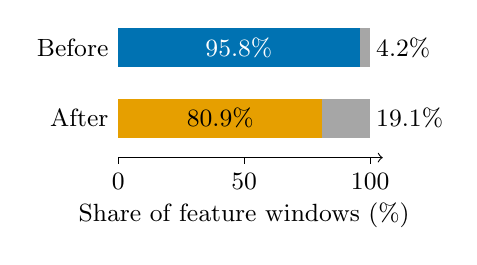
\begin{tikzpicture}[font=\small, x=0.032cm, y=1cm]
			% shares of the states in percent, before and after the amount drift
			\node[left] at (0, 1.4) {Before};
			\fill[stateA] (0, 1.15) rectangle (95.8, 1.65);
			\fill[black!35] (95.8, 1.15) rectangle (100, 1.65);
			\node[right, inner sep=2pt] at (100, 1.4) {4.2\%};
			\node[text=white] at (47.9, 1.4) {95.8\%};
			\node[left] at (0, 0.5) {After};
			\fill[stateB] (0, 0.25) rectangle (80.9, 0.75);
			\fill[black!35] (80.9, 0.25) rectangle (100, 0.75);
			\node at (40.5, 0.5) {80.9\%};
			\node[right, inner sep=2pt] at (100, 0.5) {19.1\%};
			\draw[->] (0, 0) -- (105, 0);
			\foreach \x in {0, 50, 100}
				\draw (\x, 0) -- (\x, -0.08) node[below] {\x};
			\node[below=0.45cm] at (50, 0) {Share of feature windows (\%)};
		\end{tikzpicture}
		\caption{State frequencies}
		\label{fig:approach:state_plots_frequencies}
	\end{subfigure}

	\medskip
	\begin{subfigure}{\textwidth}
		\centering
		% generated by notebooks/thesis, do not edit by hand
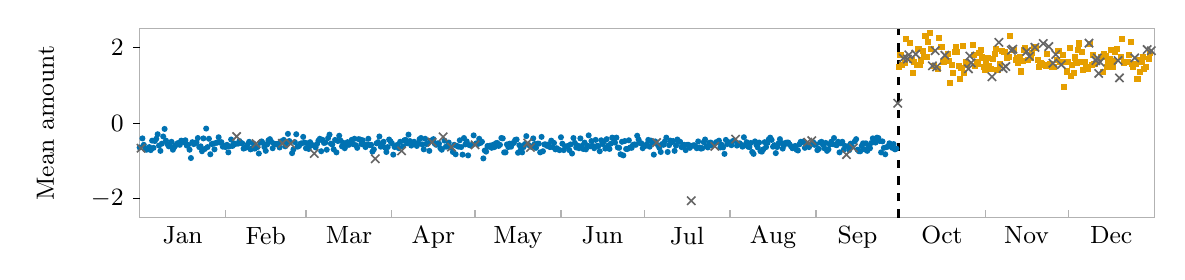
\begin{tikzpicture}[font=\small, x=0.0352cm, y=0.480cm]
	\draw[black!30] (0, -2.50) rectangle (366, 2.50);
	\node[below, inner sep=1pt] at (15.5, -2.65) {Jan};
	\node[below, inner sep=1pt] at (45.5, -2.65) {Feb};
	\draw[black!30] (31.0, -2.50) -- (31.0, -2.30);
	\node[below, inner sep=1pt] at (75.5, -2.65) {Mar};
	\draw[black!30] (60.0, -2.50) -- (60.0, -2.30);
	\node[below, inner sep=1pt] at (106.0, -2.65) {Apr};
	\draw[black!30] (91.0, -2.50) -- (91.0, -2.30);
	\node[below, inner sep=1pt] at (136.5, -2.65) {May};
	\draw[black!30] (121.0, -2.50) -- (121.0, -2.30);
	\node[below, inner sep=1pt] at (167.0, -2.65) {Jun};
	\draw[black!30] (152.0, -2.50) -- (152.0, -2.30);
	\node[below, inner sep=1pt] at (197.5, -2.65) {Jul};
	\draw[black!30] (182.0, -2.50) -- (182.0, -2.30);
	\node[below, inner sep=1pt] at (228.5, -2.65) {Aug};
	\draw[black!30] (213.0, -2.50) -- (213.0, -2.30);
	\node[below, inner sep=1pt] at (259.0, -2.65) {Sep};
	\draw[black!30] (244.0, -2.50) -- (244.0, -2.30);
	\node[below, inner sep=1pt] at (289.5, -2.65) {Oct};
	\draw[black!30] (274.0, -2.50) -- (274.0, -2.30);
	\node[below, inner sep=1pt] at (320.0, -2.65) {Nov};
	\draw[black!30] (305.0, -2.50) -- (305.0, -2.30);
	\node[below, inner sep=1pt] at (350.5, -2.65) {Dec};
	\draw[black!30] (335.0, -2.50) -- (335.0, -2.30);
	\draw (0, -2.00) -- ++(-0.08cm, 0) node[left] {$-2$};
	\draw (0, 0.00) -- ++(-0.08cm, 0) node[left] {$0$};
	\draw (0, 2.00) -- ++(-0.08cm, 0) node[left] {$2$};
	\node[rotate=90] at (-34, 0.00) {Mean amount};
	\draw[dashed, thick] (273.75, -2.50) -- (273.75, 2.50);
	\foreach \x/\y in {0.00/-0.64, 1.00/-0.40, 1.50/-0.57, 2.00/-0.69, 2.50/-0.70, 3.00/-0.67, 3.50/-0.63, 4.00/-0.71, 4.50/-0.46, 5.00/-0.65, 5.50/-0.47, 6.00/-0.41, 6.50/-0.29, 7.00/-0.59, 7.50/-0.73, 8.00/-0.54, 8.50/-0.35, 9.00/-0.15, 9.50/-0.46, 10.00/-0.55, 10.50/-0.61, 11.00/-0.60, 11.50/-0.49, 12.00/-0.70, 12.50/-0.63, 13.00/-0.58, 13.50/-0.54, 14.00/-0.52, 14.50/-0.57, 15.00/-0.46, 15.50/-0.47, 16.00/-0.50, 16.50/-0.45, 17.00/-0.59, 17.50/-0.57, 18.00/-0.70, 18.50/-0.92, 19.00/-0.50, 19.50/-0.55, 20.00/-0.53, 20.50/-0.50, 21.00/-0.39, 21.50/-0.63, 22.00/-0.61, 22.50/-0.74, 23.00/-0.40, 23.50/-0.68, 24.00/-0.14, 24.50/-0.63, 25.00/-0.41, 25.50/-0.82, 26.00/-0.55, 26.50/-0.54, 27.00/-0.69, 27.50/-0.52, 28.00/-0.51, 28.50/-0.37, 29.00/-0.51, 29.50/-0.50, 30.00/-0.62, 30.50/-0.60, 31.00/-0.63, 31.50/-0.57, 32.00/-0.77, 32.50/-0.61, 33.00/-0.43, 33.50/-0.60, 34.00/-0.53, 34.50/-0.55, 35.50/-0.54, 36.00/-0.47, 36.50/-0.52, 37.00/-0.53, 37.50/-0.67, 38.00/-0.65, 38.50/-0.64, 39.00/-0.56, 39.50/-0.49, 40.00/-0.69, 40.50/-0.67, 41.00/-0.53, 41.50/-0.67, 42.50/-0.63, 43.00/-0.80, 43.50/-0.51, 44.00/-0.48, 44.50/-0.52, 45.00/-0.63, 45.50/-0.73, 46.00/-0.56, 46.50/-0.45, 47.00/-0.42, 47.50/-0.49, 48.00/-0.66, 48.50/-0.54, 49.00/-0.55, 49.50/-0.55, 50.00/-0.54, 50.50/-0.64, 51.00/-0.48, 52.00/-0.44, 52.50/-0.61, 53.00/-0.51, 53.50/-0.28, 54.00/-0.47, 55.00/-0.79, 55.50/-0.69, 56.00/-0.50, 56.50/-0.29, 57.00/-0.62, 57.50/-0.60, 58.00/-0.54, 58.50/-0.53, 59.00/-0.36, 59.50/-0.51, 60.00/-0.66, 60.50/-0.53, 61.00/-0.68, 61.50/-0.50, 62.00/-0.58, 62.50/-0.58, 63.50/-0.64, 64.00/-0.55, 64.50/-0.46, 65.00/-0.41, 65.50/-0.74, 66.00/-0.44, 66.50/-0.52, 67.00/-0.51, 67.50/-0.70, 68.00/-0.39, 68.50/-0.30, 69.00/-0.54, 69.50/-0.56, 70.00/-0.69, 70.50/-0.44, 71.00/-0.77, 71.50/-0.47, 72.00/-0.33, 72.50/-0.46, 73.00/-0.61, 73.50/-0.52, 74.00/-0.66, 74.50/-0.58, 75.00/-0.50, 75.50/-0.57, 76.00/-0.51, 76.50/-0.44, 77.00/-0.55, 77.50/-0.41, 78.00/-0.58, 78.50/-0.65, 79.00/-0.42, 79.50/-0.43, 80.00/-0.55, 80.50/-0.45, 81.00/-0.57, 81.50/-0.63, 82.00/-0.56, 82.50/-0.41, 83.00/-0.58, 83.50/-0.57, 84.00/-0.75, 84.50/-0.69, 85.50/-0.53, 86.00/-0.50, 86.50/-0.35, 87.00/-0.62, 87.50/-0.58, 88.00/-0.49, 88.50/-0.64, 89.00/-0.76, 89.50/-0.63, 90.00/-0.43, 90.50/-0.48, 91.00/-0.53, 91.50/-0.83, 92.00/-0.63, 92.50/-0.60, 93.00/-0.57, 93.50/-0.66, 94.00/-0.49, 95.00/-0.61, 95.50/-0.45, 96.00/-0.44, 96.50/-0.53, 97.00/-0.30, 97.50/-0.47, 98.00/-0.59, 98.50/-0.55, 99.00/-0.49, 99.50/-0.53, 100.00/-0.60, 100.50/-0.54, 101.00/-0.42, 101.50/-0.39, 102.00/-0.56, 102.50/-0.69, 103.00/-0.41, 103.50/-0.55, 104.00/-0.53, 104.50/-0.73, 105.00/-0.46, 106.00/-0.42, 106.50/-0.54, 107.00/-0.57, 107.50/-0.53, 108.00/-0.54, 108.50/-0.66, 109.00/-0.70, 110.00/-0.46, 110.50/-0.62, 111.00/-0.61, 111.50/-0.51, 112.00/-0.64, 113.00/-0.76, 113.50/-0.57, 114.00/-0.82, 114.50/-0.60, 115.00/-0.62, 115.50/-0.45, 116.00/-0.63, 116.50/-0.83, 117.00/-0.39, 117.50/-0.56, 118.00/-0.48, 118.50/-0.85, 119.00/-0.58, 119.50/-0.59, 120.00/-0.57, 120.50/-0.32, 121.50/-0.53, 122.00/-0.55, 122.50/-0.41, 123.00/-0.52, 123.50/-0.49, 124.00/-0.93, 124.50/-0.72, 125.00/-0.75, 125.50/-0.60, 126.00/-0.62, 126.50/-0.59, 127.00/-0.65, 127.50/-0.57, 128.00/-0.63, 128.50/-0.53, 129.00/-0.52, 129.50/-0.60, 130.00/-0.57, 130.50/-0.39, 131.00/-0.40, 131.50/-0.77, 132.00/-0.77, 132.50/-0.56, 133.00/-0.63, 133.50/-0.54, 134.00/-0.62, 134.50/-0.53, 135.00/-0.52, 135.50/-0.44, 136.00/-0.43, 136.50/-0.78, 137.00/-0.58, 137.50/-0.70, 138.00/-0.77, 138.50/-0.63, 139.00/-0.55, 139.50/-0.34, 140.50/-0.58, 141.50/-0.63, 142.00/-0.40, 142.50/-0.55, 143.00/-0.65, 143.50/-0.54, 144.00/-0.54, 144.50/-0.77, 145.00/-0.36, 145.50/-0.74, 146.00/-0.56, 146.50/-0.56, 147.00/-0.60, 147.50/-0.56, 148.00/-0.63, 148.50/-0.46, 149.00/-0.63, 149.50/-0.52, 150.00/-0.69, 150.50/-0.66, 151.00/-0.69, 151.50/-0.71, 152.00/-0.37, 152.50/-0.54, 153.00/-0.71, 153.50/-0.61, 154.00/-0.62, 154.50/-0.60, 155.00/-0.71, 155.50/-0.56, 156.00/-0.80, 156.50/-0.39, 157.00/-0.52, 157.50/-0.64, 158.00/-0.59, 158.50/-0.66, 159.00/-0.40, 159.50/-0.60, 160.00/-0.68, 160.50/-0.51, 161.00/-0.69, 161.50/-0.59, 162.00/-0.32, 162.50/-0.61, 163.00/-0.47, 163.50/-0.60, 164.00/-0.66, 164.50/-0.44, 165.00/-0.60, 165.50/-0.60, 166.00/-0.74, 166.50/-0.45, 167.00/-0.55, 167.50/-0.48, 168.00/-0.67, 168.50/-0.42, 169.00/-0.59, 169.50/-0.68, 170.00/-0.54, 170.50/-0.38, 171.00/-0.41, 171.50/-0.51, 172.00/-0.38, 172.50/-0.64, 173.00/-0.65, 173.50/-0.82, 174.00/-0.49, 174.50/-0.85, 175.00/-0.47, 175.50/-0.68, 176.00/-0.68, 176.50/-0.45, 177.00/-0.64, 177.50/-0.65, 178.00/-0.57, 178.50/-0.56, 179.00/-0.57, 179.50/-0.33, 180.00/-0.43, 180.50/-0.52, 181.00/-0.53, 181.50/-0.66, 182.00/-0.59, 182.50/-0.60, 183.00/-0.55, 183.50/-0.44, 184.00/-0.62, 184.50/-0.46, 185.00/-0.51, 185.50/-0.83, 186.00/-0.48, 187.00/-0.58, 187.50/-0.65, 188.00/-0.76, 188.50/-0.55, 189.00/-0.57, 189.50/-0.48, 190.00/-0.38, 190.50/-0.76, 191.00/-0.58, 191.50/-0.46, 192.00/-0.50, 192.50/-0.47, 193.00/-0.73, 193.50/-0.59, 194.00/-0.43, 194.50/-0.49, 195.00/-0.49, 195.50/-0.63, 196.00/-0.62, 196.50/-0.57, 197.00/-0.71, 197.50/-0.57, 198.00/-0.57, 198.50/-0.65, 199.50/-0.59, 200.00/-0.58, 200.50/-0.61, 201.00/-0.66, 201.50/-0.48, 202.00/-0.64, 202.50/-0.67, 203.00/-0.66, 203.50/-0.50, 204.00/-0.43, 204.50/-0.61, 205.00/-0.64, 205.50/-0.52, 206.00/-0.51, 206.50/-0.58, 207.00/-0.56, 208.00/-0.50, 208.50/-0.50, 209.00/-0.46, 209.50/-0.64, 210.00/-0.57, 210.50/-0.64, 211.00/-0.81, 211.50/-0.44, 212.00/-0.55, 212.50/-0.50, 213.00/-0.52, 213.50/-0.58, 214.00/-0.47, 214.50/-0.46, 215.50/-0.59, 216.00/-0.54, 216.50/-0.53, 217.00/-0.57, 217.50/-0.62, 218.00/-0.37, 218.50/-0.57, 219.00/-0.50, 219.50/-0.62, 220.00/-0.63, 220.50/-0.52, 221.00/-0.76, 221.50/-0.81, 222.00/-0.48, 222.50/-0.57, 223.00/-0.64, 223.50/-0.51, 224.00/-0.74, 224.50/-0.75, 225.00/-0.69, 225.50/-0.50, 226.00/-0.63, 226.50/-0.52, 227.00/-0.42, 227.50/-0.38, 228.00/-0.44, 228.50/-0.62, 229.00/-0.58, 229.50/-0.79, 230.00/-0.63, 230.50/-0.53, 231.00/-0.42, 231.50/-0.52, 232.00/-0.67, 232.50/-0.58, 233.00/-0.52, 233.50/-0.51, 234.00/-0.51, 234.50/-0.56, 235.00/-0.61, 235.50/-0.66, 236.00/-0.64, 236.50/-0.60, 237.00/-0.70, 237.50/-0.72, 238.00/-0.56, 238.50/-0.49, 239.00/-0.50, 239.50/-0.48, 240.00/-0.65, 240.50/-0.54, 241.50/-0.63, 242.00/-0.56, 243.00/-0.50, 243.50/-0.57, 244.00/-0.56, 244.50/-0.71, 245.00/-0.68, 245.50/-0.51, 246.00/-0.49, 246.50/-0.56, 247.00/-0.66, 247.50/-0.52, 248.00/-0.73, 248.50/-0.69, 249.00/-0.56, 249.50/-0.49, 250.00/-0.55, 250.50/-0.39, 251.00/-0.57, 251.50/-0.58, 252.00/-0.49, 252.50/-0.77, 253.00/-0.53, 253.50/-0.49, 254.00/-0.70, 254.50/-0.60, 255.50/-0.61, 256.00/-0.71, 256.50/-0.54, 257.00/-0.62, 258.00/-0.48, 258.50/-0.42, 259.00/-0.70, 259.50/-0.74, 260.00/-0.74, 260.50/-0.60, 261.00/-0.53, 261.50/-0.69, 262.00/-0.53, 262.50/-0.73, 263.00/-0.60, 263.50/-0.66, 264.00/-0.52, 264.50/-0.40, 265.00/-0.46, 265.50/-0.51, 266.00/-0.38, 266.50/-0.39, 267.00/-0.47, 267.50/-0.77, 268.00/-0.48, 268.50/-0.65, 269.00/-0.82, 269.50/-0.63, 270.00/-0.61, 270.50/-0.53, 271.00/-0.56, 271.50/-0.65, 272.00/-0.55, 272.50/-0.69, 273.00/-0.67} \fill[stateA] (\x, \y) circle (1.1pt);
	\foreach \x/\y in {274.00/1.48, 274.50/1.81, 275.00/1.54, 276.00/1.60, 276.50/2.22, 278.00/2.12, 278.50/1.68, 279.00/1.33, 279.50/1.62, 280.50/1.54, 281.00/1.97, 281.50/1.54, 282.00/1.66, 282.50/1.92, 283.00/1.75, 283.50/2.31, 284.00/1.76, 284.50/2.16, 285.00/2.38, 285.50/1.97, 286.50/1.51, 288.00/1.43, 288.50/2.26, 289.00/2.03, 289.50/2.03, 290.00/1.62, 291.00/1.71, 291.50/1.83, 292.00/1.65, 292.50/1.07, 293.00/1.55, 293.50/1.33, 294.00/1.88, 294.50/2.02, 295.00/1.88, 295.50/1.51, 296.00/1.17, 296.50/1.46, 297.00/2.04, 297.50/1.32, 298.00/1.63, 298.50/1.54, 300.50/2.07, 301.00/1.81, 301.50/1.52, 302.00/1.62, 302.50/1.57, 303.00/1.86, 303.50/1.93, 304.00/1.74, 304.50/1.49, 305.00/1.41, 305.50/1.62, 306.00/1.72, 306.50/1.51, 307.00/1.44, 308.00/1.70, 308.50/1.84, 309.00/1.97, 309.50/1.41, 310.50/1.57, 311.00/1.91, 312.00/1.89, 313.00/1.73, 313.50/1.76, 314.00/2.31, 315.50/1.95, 316.00/1.67, 316.50/1.73, 317.00/1.60, 317.50/1.76, 318.00/1.37, 318.50/1.64, 319.00/1.95, 319.50/2.00, 320.50/1.67, 321.50/1.74, 322.00/1.86, 322.50/2.01, 323.50/1.99, 324.00/1.67, 324.50/1.49, 325.00/1.59, 325.50/1.57, 326.50/1.54, 327.00/1.51, 327.50/1.84, 328.50/1.57, 329.00/1.48, 330.00/1.48, 331.00/1.68, 331.50/1.91, 332.00/1.61, 333.00/1.80, 333.50/0.95, 334.00/1.61, 334.50/1.37, 335.00/1.63, 335.50/2.00, 336.00/1.26, 336.50/1.53, 337.00/1.33, 337.50/1.74, 338.00/1.60, 338.50/1.93, 339.00/2.11, 339.50/1.63, 340.00/1.88, 340.50/1.42, 341.00/1.63, 341.50/1.48, 342.00/1.45, 343.00/2.10, 343.50/1.55, 344.00/1.81, 344.50/1.58, 347.00/1.76, 347.50/1.36, 348.00/1.84, 348.50/1.78, 349.00/1.50, 349.50/1.66, 350.00/1.71, 350.50/1.95, 351.00/1.49, 351.50/1.65, 352.00/1.88, 352.50/1.97, 354.00/1.76, 354.50/2.22, 355.00/1.59, 355.50/1.61, 356.00/1.62, 356.50/1.61, 357.00/1.80, 357.50/2.16, 358.00/1.58, 358.50/1.49, 359.50/1.58, 360.00/1.18, 360.50/1.68, 361.00/1.36, 361.50/1.63, 362.00/1.76, 362.50/1.43, 363.00/1.48, 364.00/1.69, 364.50/1.85} \fill[stateB] (\x, \y) ++(-1.1pt, -1.1pt) rectangle ++(2.2pt, 2.2pt);
	\foreach \x/\y in {0.50/-0.66, 35.00/-0.35, 42.00/-0.54, 51.50/-0.53, 54.50/-0.54, 63.00/-0.80, 85.00/-0.94, 94.50/-0.73, 105.50/-0.50, 109.50/-0.36, 112.50/-0.63, 121.00/-0.57, 140.00/-0.52, 141.00/-0.64, 186.50/-0.51, 199.00/-2.05, 207.50/-0.61, 215.00/-0.42, 241.00/-0.50, 242.50/-0.46, 255.00/-0.83, 257.50/-0.65, 273.50/0.53, 275.50/1.72, 277.00/1.70, 277.50/1.81, 280.00/1.83, 286.00/1.52, 287.00/1.92, 287.50/1.49, 290.50/1.80, 299.00/1.44, 299.50/1.78, 300.00/1.60, 307.50/1.23, 310.00/2.14, 311.50/1.45, 312.50/1.50, 314.50/1.93, 315.00/1.96, 320.00/1.90, 321.00/1.77, 323.00/2.01, 326.00/2.11, 328.00/2.03, 329.50/1.59, 330.50/1.82, 332.50/1.55, 342.50/2.12, 345.00/1.66, 345.50/1.73, 346.00/1.32, 346.50/1.62, 353.00/1.66, 353.50/1.20, 359.00/1.73, 363.50/1.95, 365.00/1.92} \draw[black!60, line width=0.6pt] (\x, \y) ++(-1.5pt, -1.5pt) -- ++(3pt, 3pt) ++(0, -3pt) -- ++(-3pt, 3pt);
\end{tikzpicture}

		\caption{Standardized mean amount of the feature windows}
		\label{fig:approach:states_inter}
	\end{subfigure}

	\medskip
	\begin{subfigure}{\textwidth}
		\centering
		% generated by notebooks/thesis, do not edit by hand
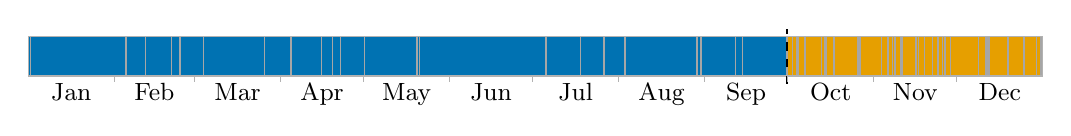
\begin{tikzpicture}[font=\small, x=0.0352cm, y=1cm]
	\fill[stateA] (0.00, 0) rectangle (0.60, 0.5);
	\fill[black!35] (0.50, 0) rectangle (1.10, 0.5);
	\fill[stateA] (1.00, 0) rectangle (35.00, 0.5);
	\fill[black!35] (35.00, 0) rectangle (35.60, 0.5);
	\fill[stateA] (35.50, 0) rectangle (42.00, 0.5);
	\fill[black!35] (42.00, 0) rectangle (42.60, 0.5);
	\fill[stateA] (42.50, 0) rectangle (51.50, 0.5);
	\fill[black!35] (51.50, 0) rectangle (52.10, 0.5);
	\fill[stateA] (52.00, 0) rectangle (54.50, 0.5);
	\fill[black!35] (54.50, 0) rectangle (55.10, 0.5);
	\fill[stateA] (55.00, 0) rectangle (63.00, 0.5);
	\fill[black!35] (63.00, 0) rectangle (63.60, 0.5);
	\fill[stateA] (63.50, 0) rectangle (85.00, 0.5);
	\fill[black!35] (85.00, 0) rectangle (85.60, 0.5);
	\fill[stateA] (85.50, 0) rectangle (94.50, 0.5);
	\fill[black!35] (94.50, 0) rectangle (95.10, 0.5);
	\fill[stateA] (95.00, 0) rectangle (105.50, 0.5);
	\fill[black!35] (105.50, 0) rectangle (106.10, 0.5);
	\fill[stateA] (106.00, 0) rectangle (109.50, 0.5);
	\fill[black!35] (109.50, 0) rectangle (110.10, 0.5);
	\fill[stateA] (110.00, 0) rectangle (112.50, 0.5);
	\fill[black!35] (112.50, 0) rectangle (113.10, 0.5);
	\fill[stateA] (113.00, 0) rectangle (121.00, 0.5);
	\fill[black!35] (121.00, 0) rectangle (121.60, 0.5);
	\fill[stateA] (121.50, 0) rectangle (140.00, 0.5);
	\fill[black!35] (140.00, 0) rectangle (140.60, 0.5);
	\fill[stateA] (140.50, 0) rectangle (141.10, 0.5);
	\fill[black!35] (141.00, 0) rectangle (141.60, 0.5);
	\fill[stateA] (141.50, 0) rectangle (186.50, 0.5);
	\fill[black!35] (186.50, 0) rectangle (187.10, 0.5);
	\fill[stateA] (187.00, 0) rectangle (199.00, 0.5);
	\fill[black!35] (199.00, 0) rectangle (199.60, 0.5);
	\fill[stateA] (199.50, 0) rectangle (207.50, 0.5);
	\fill[black!35] (207.50, 0) rectangle (208.10, 0.5);
	\fill[stateA] (208.00, 0) rectangle (215.00, 0.5);
	\fill[black!35] (215.00, 0) rectangle (215.60, 0.5);
	\fill[stateA] (215.50, 0) rectangle (241.00, 0.5);
	\fill[black!35] (241.00, 0) rectangle (241.60, 0.5);
	\fill[stateA] (241.50, 0) rectangle (242.50, 0.5);
	\fill[black!35] (242.50, 0) rectangle (243.10, 0.5);
	\fill[stateA] (243.00, 0) rectangle (255.00, 0.5);
	\fill[black!35] (255.00, 0) rectangle (255.60, 0.5);
	\fill[stateA] (255.50, 0) rectangle (257.50, 0.5);
	\fill[black!35] (257.50, 0) rectangle (258.10, 0.5);
	\fill[stateA] (258.00, 0) rectangle (273.50, 0.5);
	\fill[black!35] (273.50, 0) rectangle (274.10, 0.5);
	\fill[stateB] (274.00, 0) rectangle (275.50, 0.5);
	\fill[black!35] (275.50, 0) rectangle (276.10, 0.5);
	\fill[stateB] (276.00, 0) rectangle (277.00, 0.5);
	\fill[black!35] (277.00, 0) rectangle (278.00, 0.5);
	\fill[stateB] (278.00, 0) rectangle (280.00, 0.5);
	\fill[black!35] (280.00, 0) rectangle (280.60, 0.5);
	\fill[stateB] (280.50, 0) rectangle (286.00, 0.5);
	\fill[black!35] (286.00, 0) rectangle (286.60, 0.5);
	\fill[stateB] (286.50, 0) rectangle (287.10, 0.5);
	\fill[black!35] (287.00, 0) rectangle (288.00, 0.5);
	\fill[stateB] (288.00, 0) rectangle (290.50, 0.5);
	\fill[black!35] (290.50, 0) rectangle (291.10, 0.5);
	\fill[stateB] (291.00, 0) rectangle (299.00, 0.5);
	\fill[black!35] (299.00, 0) rectangle (300.50, 0.5);
	\fill[stateB] (300.50, 0) rectangle (307.50, 0.5);
	\fill[black!35] (307.50, 0) rectangle (308.10, 0.5);
	\fill[stateB] (308.00, 0) rectangle (310.00, 0.5);
	\fill[black!35] (310.00, 0) rectangle (310.60, 0.5);
	\fill[stateB] (310.50, 0) rectangle (311.50, 0.5);
	\fill[black!35] (311.50, 0) rectangle (312.10, 0.5);
	\fill[stateB] (312.00, 0) rectangle (312.60, 0.5);
	\fill[black!35] (312.50, 0) rectangle (313.10, 0.5);
	\fill[stateB] (313.00, 0) rectangle (314.50, 0.5);
	\fill[black!35] (314.50, 0) rectangle (315.50, 0.5);
	\fill[stateB] (315.50, 0) rectangle (320.00, 0.5);
	\fill[black!35] (320.00, 0) rectangle (320.60, 0.5);
	\fill[stateB] (320.50, 0) rectangle (321.10, 0.5);
	\fill[black!35] (321.00, 0) rectangle (321.60, 0.5);
	\fill[stateB] (321.50, 0) rectangle (323.00, 0.5);
	\fill[black!35] (323.00, 0) rectangle (323.60, 0.5);
	\fill[stateB] (323.50, 0) rectangle (326.00, 0.5);
	\fill[black!35] (326.00, 0) rectangle (326.60, 0.5);
	\fill[stateB] (326.50, 0) rectangle (328.00, 0.5);
	\fill[black!35] (328.00, 0) rectangle (328.60, 0.5);
	\fill[stateB] (328.50, 0) rectangle (329.50, 0.5);
	\fill[black!35] (329.50, 0) rectangle (330.10, 0.5);
	\fill[stateB] (330.00, 0) rectangle (330.60, 0.5);
	\fill[black!35] (330.50, 0) rectangle (331.10, 0.5);
	\fill[stateB] (331.00, 0) rectangle (332.50, 0.5);
	\fill[black!35] (332.50, 0) rectangle (333.10, 0.5);
	\fill[stateB] (333.00, 0) rectangle (342.50, 0.5);
	\fill[black!35] (342.50, 0) rectangle (343.10, 0.5);
	\fill[stateB] (343.00, 0) rectangle (345.00, 0.5);
	\fill[black!35] (345.00, 0) rectangle (347.00, 0.5);
	\fill[stateB] (347.00, 0) rectangle (353.00, 0.5);
	\fill[black!35] (353.00, 0) rectangle (354.00, 0.5);
	\fill[stateB] (354.00, 0) rectangle (359.00, 0.5);
	\fill[black!35] (359.00, 0) rectangle (359.60, 0.5);
	\fill[stateB] (359.50, 0) rectangle (363.50, 0.5);
	\fill[black!35] (363.50, 0) rectangle (364.10, 0.5);
	\fill[stateB] (364.00, 0) rectangle (365.00, 0.5);
	\fill[black!35] (365.00, 0) rectangle (365.60, 0.5);
	\draw[black!30] (0, 0) rectangle (366, 0.5);
	\draw[dashed, thick] (273.75, -0.1) -- (273.75, 0.6);
	\node[below, inner sep=1pt] at (15.5, -0.05) {Jan};
	\node[below, inner sep=1pt] at (45.5, -0.05) {Feb};
	\draw[black!30] (31.0, 0) -- (31.0, -0.08);
	\node[below, inner sep=1pt] at (75.5, -0.05) {Mar};
	\draw[black!30] (60.0, 0) -- (60.0, -0.08);
	\node[below, inner sep=1pt] at (106.0, -0.05) {Apr};
	\draw[black!30] (91.0, 0) -- (91.0, -0.08);
	\node[below, inner sep=1pt] at (136.5, -0.05) {May};
	\draw[black!30] (121.0, 0) -- (121.0, -0.08);
	\node[below, inner sep=1pt] at (167.0, -0.05) {Jun};
	\draw[black!30] (152.0, 0) -- (152.0, -0.08);
	\node[below, inner sep=1pt] at (197.5, -0.05) {Jul};
	\draw[black!30] (182.0, 0) -- (182.0, -0.08);
	\node[below, inner sep=1pt] at (228.5, -0.05) {Aug};
	\draw[black!30] (213.0, 0) -- (213.0, -0.08);
	\node[below, inner sep=1pt] at (259.0, -0.05) {Sep};
	\draw[black!30] (244.0, 0) -- (244.0, -0.08);
	\node[below, inner sep=1pt] at (289.5, -0.05) {Oct};
	\draw[black!30] (274.0, 0) -- (274.0, -0.08);
	\node[below, inner sep=1pt] at (320.0, -0.05) {Nov};
	\draw[black!30] (305.0, 0) -- (305.0, -0.08);
	\node[below, inner sep=1pt] at (350.5, -0.05) {Dec};
	\draw[black!30] (335.0, 0) -- (335.0, -0.08);
\end{tikzpicture}

		\caption{Trajectory of the event log}
		\label{fig:approach:trajectories_inter}
	\end{subfigure}
	\caption[Inter-case clustering of the running example]{%
		DBSCAN clustering of the inter-case features of the running example $L_3$ (Example~\ref{ex:approach:clustering_inter}). Blue is state~1, orange state~2 and gray noise.
		\subref{fig:approach:cluster_eval_dbscan}~Sorted 8-distance graph with the chosen radius $\varepsilon = 0.7$ (dashed), cut at 3.
		\subref{fig:approach:state_plots_frequencies}~Shares of the states before and after the amount drift.
		\subref{fig:approach:states_inter}~Each symbol is a feature window. Since DBSCAN also uses the other three features, some noise lies within the clusters.
		\subref{fig:approach:trajectories_inter}~Each box is a visit of a state.
		In \subref{fig:approach:states_inter} and \subref{fig:approach:trajectories_inter}, dashed lines mark the amount drift.}
	\label{fig:approach:clustering_inter}
\end{figure}

\begin{example}
	\label{ex:approach:clustering_inter}
	We choose DBSCAN, which marks unusual feature windows as noise instead of forcing them into a state. We cluster the four standardized inter-case features of $L_3$ (Example~\ref{ex:approach:reduction_inter}) with $\mathit{minPts} = 8$, i.e., twice the number of features. The sorted 8-distance graph rises gradually and only steeply for a few outliers, so it has no clear knee (Figure~\ref{fig:approach:cluster_eval_dbscan}). The largest 8-distance of 13.06 belongs to the empty feature window of July~18, 00:00, with the standardized mean gap $-14.53$. Therefore, we compare the radii $\varepsilon \in \Set{0.6, 0.7, 0.8, 0.9}$ with DBCV, and $\varepsilon = 0.7$ reaches the highest DBCV of 0.141.
	\begin{itemize}
		\item State~1 contains 525 feature windows before the amount drift, and state~2 contains 148 after it (Figure~\ref{fig:approach:states_inter}). The remaining 58 feature windows are noise.

		\item The feature window of September~30, 12:00, contains cases before and after the drift. Its standardized mean amount of 0.53 lies between both clusters, so it is noise.

		\item Before the drift, 4.2\% of the feature windows are noise, and after it 19.1\% (Figure~\ref{fig:approach:state_plots_frequencies}).

		\item The trajectory of the event log has 98 visits (Figure~\ref{fig:approach:trajectories_inter}). State~1 has 23 visits of up to 45 days and state~2 has 26 visits of up to 9.5 days. The 49 visits of the noise last at most 2 days and only briefly interrupt the visits of the clusters.

		\item For $\varepsilon \ge 1.0$, DBSCAN merges both clusters into one state, and the drift disappears from the states.
	\end{itemize}
\end{example}

Table~\ref{tab:approach:cluster_eval} compares the chosen clusterings of the three perspectives. In the intra-case and the resource perspective, the drift clearly separates the rows, so the silhouettes reach 0.857 and 0.934. In the inter-case perspective, the drift only changes one of the four features, and the other features scatter the clusters. Thus, the silhouette of 0.382 and the DBCV of 0.141 stay low, although the states show the drift. The Cali\'nski--Harabasz index depends on the scale of the features and thus only compares clusterings of the same perspective.

\section{Drift Signals}
\label{sec:approach:drift_signals}
A state describes a single row, whereas a drift describes a change over time. Since all process versions share the same states, a drift can be seen in how often each state occurs. A state that only occurs after a drift has the frequency 0 before the drift. A drift signal makes these changes measurable. For each signal window, we count how often the rows have the states and obtain a state distribution. A divergence compares these state distributions with a reference, e.g., the state distribution of the previous signal window. The divergence of a signal window is the drift score of that signal window. The time series of drift scores over the signal windows is the drift signal.

Clustering-based detectors observe how the composition of clusters changes over time (\textcite{sato2022survey}). The drift signal quantifies this change for each signal window. The comparison with a reference follows the window-based detectors. ProDrift compares the distribution of the runs of a reference window and a detection window using a $\chi^2$ test (\textcite{maaradji2017detecting}). In our framework, we compare states instead of runs. Therefore, this step works the same way in all three perspectives.

Our framework uses the four divergences of Section~\ref{sec:prelim:divergences}, which kairo implements as \texttt{kl}, \texttt{js}, \texttt{tv} and \texttt{hellinger} (Section~\ref{sec:impl:kairo}).

\begin{definition}[State Distributions, Drift Scores and Drift Signal]
	\label{def:approach:drift_signal}
	Let $Z \in \R^{m \times d}$ be a reduced matrix with the rows $\mathbf{z}_1^\top, \dots, \mathbf{z}_m^\top$ (Definition~\ref{def:approach:reduction}), let $K$ be the set of states with $\mathit{state}(\mathbf{z}_j) \in K$ for $1 \le j \le m$ (Definition~\ref{def:approach:states}), and let signal windows of the length $\Delta_s$ be given (Definition~\ref{def:approach:window_roles}).
	\begin{itemize}
		\item For $1 \le j \le m$, $\mathit{time}(\mathbf{z}_j)$ is the time of the row $\mathbf{z}_j$, i.e., the timestamp of its event in the intra-case perspective and the start of its feature window in the resource and inter-case perspectives.
		\item For a signal window $v$, $J_v = \Set{j \in \Set{1, \dots, m} \given \mathit{time}(\mathbf{z}_j) \in v}$ is the set of its rows.
		\item $v_1, \dots, v_n$ are the signal windows with $J_{v_i} \neq \emptyset$ in chronological order, and $t_i$ is the start of $v_i$.
		\item The state distribution of $v_i$ is $p_i \in K \to [0, 1]$ with
		      \[
			      p_i(\kappa) = \frac{\abs{\Set{j \in J_{v_i} \given \mathit{state}(\mathbf{z}_j) = \kappa}}}{\abs{J_{v_i}}} \quad\text{for } \kappa \in K.
		      \]
		\item For $i_0 \le i \le n$, the reference $q_i$ of $v_i$ is one of the following distributions over $K$, where we take means of distributions separately for each $\kappa \in K$:
		      \begin{itemize}
			      \item \emph{previous signal window} (\texttt{previous}): $q_i = p_{i-1}$ with $i_0 = 2$,
			      \item \emph{mean of the $h$ previous signal windows} (\texttt{recent}): $q_i = \frac{1}{h} \sum_{l = i-h}^{i-1} p_l$ for an $h \in \N$ with $i_0 = h + 1$,
			      \item \emph{mean of all signal windows} (\texttt{baseline}): $q_i = \frac{1}{n} \sum_{l=1}^{n} p_l$ with $i_0 = 1$.
		      \end{itemize}
		\item For a divergence $D$ of Definition~\ref{def:prelim:divergences}, $\mathit{score}_i = D(p_i, q_i)$ is the drift score of $v_i$ for $i_0 \le i \le n$.
		\item The drift signal is the sequence $\seq{(t_{i_0}, \mathit{score}_{i_0}), \dots, (t_n, \mathit{score}_n)}$.
	\end{itemize}
\end{definition}

\noindent\emph{Properties:}
\begin{itemize}[beginpenalty=10000]
	\item Each divergence is 0 for $p_i = q_i$ (Section~\ref{sec:prelim:divergences}).
	\item A high drift score indicates that the state distribution of a signal window diverges from its reference.
	\item If a state from the signal window does not occur in the reference, the drift score based on the KL divergence $D_{\mathrm{KL}}(p_i, q_i)$ is infinite.
	\item The divergences only compare the shares of the states but not their similarities.
	\item A transition into a similar state, thus, counts as much as a transition to a very different state.
\end{itemize}

The reference determines which changes the drift score measures:
\begin{itemize}[beginpenalty=10000]
	\item \emph{Previous signal window}: This reference compares neighboring signal windows. A sudden drift causes a spike in the first signal window after it. The drift score drops afterwards since the state shares of the signal windows are similar again. Random fluctuations can also cause a false positive spike in the drift score of a signal window.
	\item \emph{Mean of the $h$ previous signal windows}: This reference fluctuates less and is more stable. For each state, it is defined over the mean of that state's share in the $h$ state distributions.
	\item \emph{Mean of all signal windows}: This reference compares each signal window with the mean behavior of the entire event log. A drift shows itself more in the form of a step between two levels instead of a spike. This reference assumes complete event logs and is not applicable for online concept drift detection.
\end{itemize}

The size $\Delta_s$ of the signal window balances fluctuations against granularity in time. A short signal window has fewer rows and can have more random fluctuations in the state distributions and divergences. A long signal window smooths the frequencies but only signals a drift point as granular as $\Delta_s$.

We should be skeptical about the drift scores at the end of an event log. The last signal window often only contains the remaining events of cases that started earlier, while no new cases arrive. Thus, only certain states occur, e.g., the states of late prefixes in the intra-case perspective, and the state distribution can be misleading without any drift. An example is the last intra-case signal window of the running example, which only holds the three events of December~31 (Figure~\ref{fig:approach:drift_signal_intra}).

Similar to the earlier steps of our pipeline, this step is also flexible. The framework is extendable to different divergences (e.g., Earth Mover's Distance) as well as to distances between the state distributions of the signal windows.

In the resource and inter-case perspectives, each row belongs to a feature window. Therefore, in these perspectives, we obtain a log-level trajectory of states from the clustering. In this case, the state vectors of the signal windows can also be compared directly using distance measures. In this thesis, we focus on our approach over frequencies and divergences. The main benefit of our choice is that it aligns the result format of the three perspectives into a drift signal.

The drift signal alone cannot decide whether there is a drift. In Chapter~\ref{chap:eval}, we detect drifts with thresholds on the drift scores, which depend on the event log and the used divergence. Since each drift signal is a time series, other well-known drift detection approaches like PELT (\textcite{adams2023explainable}) or ADWIN (\textcite{baier2020handling}) can be used with those drift signals.

\begin{figure}[tb]
	\centering
	\definecolor{stateA}{RGB}{0,114,178}
	\definecolor{stateB}{RGB}{230,159,0}
	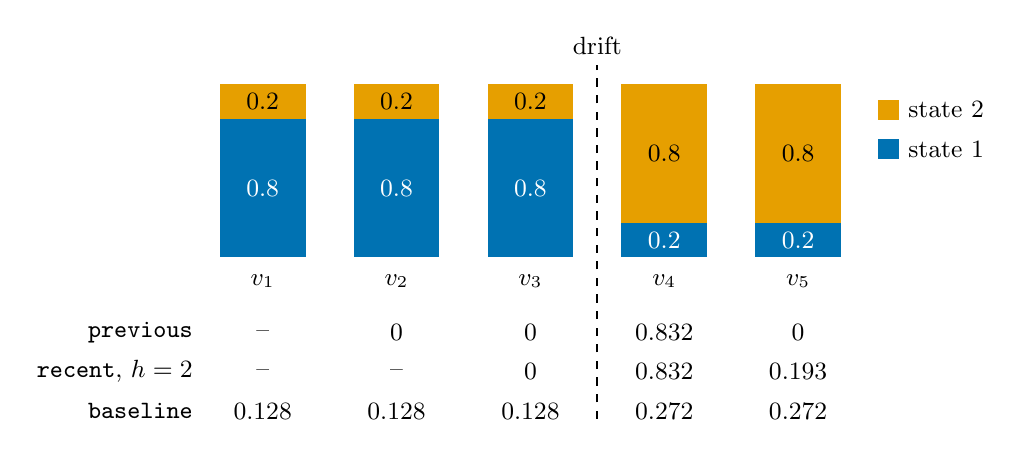
\begin{tikzpicture}[font=\small, x=1.7cm, y=1cm]
		% state distributions of the five signal windows, a share of 1 is 2.2 cm high
		\foreach \i/\a/\b in {1/0.8/0.2, 2/0.8/0.2, 3/0.8/0.2, 4/0.2/0.8, 5/0.2/0.8} {
			\fill[stateA] (\i - 0.32, 0) rectangle (\i + 0.32, 2.2 * \a);
			\fill[stateB] (\i - 0.32, 2.2 * \a) rectangle (\i + 0.32, 2.2);
			\node[text=white] at (\i, 1.1 * \a) {\a};
			\node at (\i, 2.2 - 1.1 * \b) {\b};
			\node at (\i, -0.3) {$v_{\i}$};
		}
		% sudden drift between v_3 and v_4
		\draw[dashed, thick] (3.5, -2.05) -- (3.5, 2.45) node[above] {drift};
		% legend
		\fill[stateB] (5.6, 1.75) rectangle ++(0.15, 0.25);
		\node[right] at (5.75, 1.875) {state 2};
		\fill[stateA] (5.6, 1.25) rectangle ++(0.15, 0.25);
		\node[right] at (5.75, 1.375) {state 1};
		% KL drift scores against the three references
		\node[anchor=east] at (0.55, -0.95) {\texttt{previous}};
		\foreach \i/\s in {1/--, 2/0, 3/0, 4/0.832, 5/0}
			\node at (\i, -0.95) {\s};
		\node[anchor=east] at (0.55, -1.45) {\texttt{recent}, $h = 2$};
		\foreach \i/\s in {1/--, 2/--, 3/0, 4/0.832, 5/0.193}
			\node at (\i, -1.45) {\s};
		\node[anchor=east] at (0.55, -1.95) {\texttt{baseline}};
		\foreach \i/\s in {1/0.128, 2/0.128, 3/0.128, 4/0.272, 5/0.272}
			\node at (\i, -1.95) {\s};
	\end{tikzpicture}
	\caption[Example of a drift signal]{%
		Drift signal of Example~\ref{ex:approach:drift_signal} with the states 1 (blue) and 2 (orange). Each bar is the state distribution of a signal window $v_i$ with the shares of both states, and the dashed line marks a sudden drift between $v_3$ and $v_4$. The rows below give the KL drift score of each signal window against the three references of Definition~\ref{def:approach:drift_signal}: the previous signal window (\texttt{previous}), the mean of the $h = 2$ previous signal windows (\texttt{recent}) and the mean of all signal windows (\texttt{baseline}). A dash marks a signal window without a reference.}
	\label{fig:approach:drift_signal_example}
\end{figure}

\begin{example}
	\label{ex:approach:drift_signal}
	Figure~\ref{fig:approach:drift_signal_example} shows five signal windows $v_1, \dots, v_5$ with the states $K = \Set{1, 2}$. We write a distribution $p$ over $K$ as $(p(1), p(2))$.
	\begin{itemize}
		\item The state distributions are $p_1 = p_2 = p_3 = (0.8, 0.2)$ and $p_4 = p_5 = (0.2, 0.8)$. Thus, 60\% of the rows move from state~1 to state~2 between $v_3$ and $v_4$.

		\item With the previous signal window as reference,
		      \[
			      \mathit{score}_4 = D_{\mathrm{KL}}(p_4, p_3) = 0.2 \log \frac{0.2}{0.8} + 0.8 \log \frac{0.8}{0.2} \approx 0.832.
		      \]
		      All other drift scores are 0, and $v_1$ has no drift score.

		\item With the mean of the $h = 2$ previous signal windows as reference, $v_4$ also gets the drift score 0.832. The reference $q_5 = (0.5, 0.5)$ still contains $v_3$, so $v_5$ gets the drift score 0.193.

		\item With the mean of all signal windows $(0.56, 0.44)$ as reference, $v_1$ to $v_3$ get the drift score 0.128 and $v_4$ and $v_5$ the drift score 0.272. Thus, the drift shows as a step. Since only two signal windows follow the drift, they lie further from the reference.
	\end{itemize}
\end{example}

\subsection{Intra-Case Perspective}
\label{sec:approach:drift_signals:intra}
In the intra-case perspective, the rows are events. A signal window counts the states of all events whose timestamps lie in it, i.e., prefixes of many cases at different positions. Thus, the state distribution shows how often each prefix occurs in a signal window. A control-flow drift changes this mix as soon as cases of the new process version produce events.

\begin{figure}[tb]
	\centering
	\begin{subfigure}{\textwidth}
		\centering
		% generated by notebooks/thesis, do not edit by hand
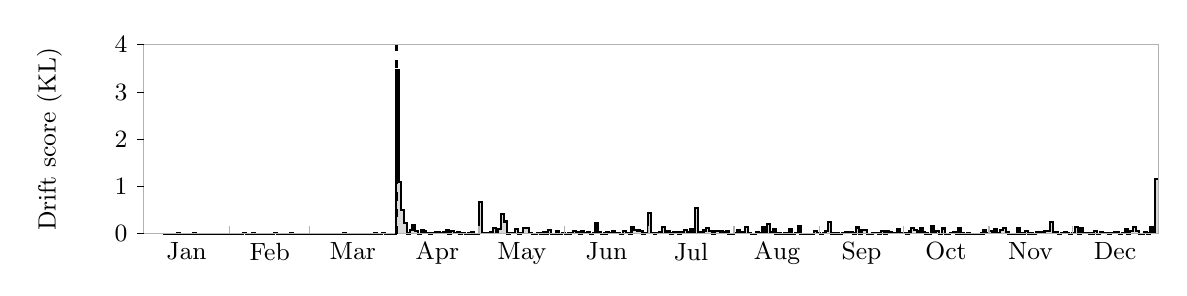
\begin{tikzpicture}[font=\small, x=0.0352cm, y=0.6000cm]
	\fill[black!15] (7.00, 0) -- (7.00, 0.0004) -- (8.00, 0.0004) -- (8.00, 0.0005) -- (9.00, 0.0005) -- (9.00, 0.0048) -- (10.00, 0.0048) -- (10.00, 0.0004) -- (11.00, 0.0004) -- (11.00, 0.0028) -- (12.00, 0.0028) -- (12.00, 0.0079) -- (13.00, 0.0079) -- (13.00, 0.0033) -- (14.00, 0.0033) -- (14.00, 0.0008) -- (15.00, 0.0008) -- (15.00, 0.0008) -- (16.00, 0.0008) -- (16.00, 0.0006) -- (17.00, 0.0006) -- (17.00, 0.0016) -- (18.00, 0.0016) -- (18.00, 0.0131) -- (19.00, 0.0131) -- (19.00, 0.0000) -- (20.00, 0.0000) -- (20.00, 0.0013) -- (21.00, 0.0013) -- (21.00, 0.0003) -- (22.00, 0.0003) -- (22.00, 0.0009) -- (23.00, 0.0009) -- (23.00, 0.0007) -- (24.00, 0.0007) -- (24.00, 0.0014) -- (25.00, 0.0014) -- (25.00, 0.0011) -- (26.00, 0.0011) -- (26.00, 0.0004) -- (27.00, 0.0004) -- (27.00, 0.0011) -- (28.00, 0.0011) -- (28.00, 0.0040) -- (29.00, 0.0040) -- (29.00, 0.0042) -- (30.00, 0.0042) -- (30.00, 0.0016) -- (31.00, 0.0016) -- (31.00, 0.0006) -- (32.00, 0.0006) -- (32.00, 0.0037) -- (33.00, 0.0037) -- (33.00, 0.0011) -- (34.00, 0.0011) -- (34.00, 0.0032) -- (35.00, 0.0032) -- (35.00, 0.0000) -- (36.00, 0.0000) -- (36.00, 0.0114) -- (37.00, 0.0114) -- (37.00, 0.0004) -- (38.00, 0.0004) -- (38.00, 0.0003) -- (39.00, 0.0003) -- (39.00, 0.0064) -- (40.00, 0.0064) -- (40.00, 0.0007) -- (41.00, 0.0007) -- (41.00, 0.0005) -- (42.00, 0.0005) -- (42.00, 0.0003) -- (43.00, 0.0003) -- (43.00, 0.0001) -- (44.00, 0.0001) -- (44.00, 0.0008) -- (45.00, 0.0008) -- (45.00, 0.0028) -- (46.00, 0.0028) -- (46.00, 0.0014) -- (47.00, 0.0014) -- (47.00, 0.0116) -- (48.00, 0.0116) -- (48.00, 0.0004) -- (49.00, 0.0004) -- (49.00, 0.0016) -- (50.00, 0.0016) -- (50.00, 0.0027) -- (51.00, 0.0027) -- (51.00, 0.0003) -- (52.00, 0.0003) -- (52.00, 0.0042) -- (53.00, 0.0042) -- (53.00, 0.0066) -- (54.00, 0.0066) -- (54.00, 0.0004) -- (55.00, 0.0004) -- (55.00, 0.0028) -- (56.00, 0.0028) -- (56.00, 0.0000) -- (57.00, 0.0000) -- (57.00, 0.0055) -- (58.00, 0.0055) -- (58.00, 0.0000) -- (59.00, 0.0000) -- (59.00, 0.0001) -- (60.00, 0.0001) -- (60.00, 0.0021) -- (61.00, 0.0021) -- (61.00, 0.0006) -- (62.00, 0.0006) -- (62.00, 0.0000) -- (63.00, 0.0000) -- (63.00, 0.0029) -- (64.00, 0.0029) -- (64.00, 0.0018) -- (65.00, 0.0018) -- (65.00, 0.0032) -- (66.00, 0.0032) -- (66.00, 0.0004) -- (67.00, 0.0004) -- (67.00, 0.0011) -- (68.00, 0.0011) -- (68.00, 0.0013) -- (69.00, 0.0013) -- (69.00, 0.0006) -- (70.00, 0.0006) -- (70.00, 0.0007) -- (71.00, 0.0007) -- (71.00, 0.0003) -- (72.00, 0.0003) -- (72.00, 0.0073) -- (73.00, 0.0073) -- (73.00, 0.0040) -- (74.00, 0.0040) -- (74.00, 0.0029) -- (75.00, 0.0029) -- (75.00, 0.0004) -- (76.00, 0.0004) -- (76.00, 0.0017) -- (77.00, 0.0017) -- (77.00, 0.0019) -- (78.00, 0.0019) -- (78.00, 0.0005) -- (79.00, 0.0005) -- (79.00, 0.0017) -- (80.00, 0.0017) -- (80.00, 0.0005) -- (81.00, 0.0005) -- (81.00, 0.0044) -- (82.00, 0.0044) -- (82.00, 0.0006) -- (83.00, 0.0006) -- (83.00, 0.0122) -- (84.00, 0.0122) -- (84.00, 0.0027) -- (85.00, 0.0027) -- (85.00, 0.0029) -- (86.00, 0.0029) -- (86.00, 0.0114) -- (87.00, 0.0114) -- (87.00, 0.0028) -- (88.00, 0.0028) -- (88.00, 0.0010) -- (89.00, 0.0010) -- (89.00, 0.0017) -- (90.00, 0.0017) -- (90.00, 0.0013) -- (91.00, 0.0013) -- (91.00, 3.4707) -- (92.00, 3.4707) -- (92.00, 1.1003) -- (93.00, 1.1003) -- (93.00, 0.4983) -- (94.00, 0.4983) -- (94.00, 0.2371) -- (95.00, 0.2371) -- (95.00, 0.0082) -- (96.00, 0.0082) -- (96.00, 0.0817) -- (97.00, 0.0817) -- (97.00, 0.1762) -- (98.00, 0.1762) -- (98.00, 0.0633) -- (99.00, 0.0633) -- (99.00, 0.0039) -- (100.00, 0.0039) -- (100.00, 0.0799) -- (101.00, 0.0799) -- (101.00, 0.0516) -- (102.00, 0.0516) -- (102.00, 0.0266) -- (103.00, 0.0266) -- (103.00, 0.0063) -- (104.00, 0.0063) -- (104.00, 0.0133) -- (105.00, 0.0133) -- (105.00, 0.0341) -- (106.00, 0.0341) -- (106.00, 0.0343) -- (107.00, 0.0343) -- (107.00, 0.0197) -- (108.00, 0.0197) -- (108.00, 0.0308) -- (109.00, 0.0308) -- (109.00, 0.0711) -- (110.00, 0.0711) -- (110.00, 0.0053) -- (111.00, 0.0053) -- (111.00, 0.0633) -- (112.00, 0.0633) -- (112.00, 0.0142) -- (113.00, 0.0142) -- (113.00, 0.0456) -- (114.00, 0.0456) -- (114.00, 0.0016) -- (115.00, 0.0016) -- (115.00, 0.0200) -- (116.00, 0.0200) -- (116.00, 0.0028) -- (117.00, 0.0028) -- (117.00, 0.0077) -- (118.00, 0.0077) -- (118.00, 0.0388) -- (119.00, 0.0388) -- (119.00, 0.0042) -- (120.00, 0.0042) -- (120.00, 0.0031) -- (121.00, 0.0031) -- (121.00, 0.6834) -- (122.00, 0.6834) -- (122.00, 0.0226) -- (123.00, 0.0226) -- (123.00, 0.0204) -- (124.00, 0.0204) -- (124.00, 0.0213) -- (125.00, 0.0213) -- (125.00, 0.0427) -- (126.00, 0.0427) -- (126.00, 0.1279) -- (127.00, 0.1279) -- (127.00, 0.0330) -- (128.00, 0.0330) -- (128.00, 0.0995) -- (129.00, 0.0995) -- (129.00, 0.4149) -- (130.00, 0.4149) -- (130.00, 0.2616) -- (131.00, 0.2616) -- (131.00, 0.0011) -- (132.00, 0.0011) -- (132.00, 0.0113) -- (133.00, 0.0113) -- (133.00, 0.0127) -- (134.00, 0.0127) -- (134.00, 0.1059) -- (135.00, 0.1059) -- (135.00, 0.0027) -- (136.00, 0.0027) -- (136.00, 0.0202) -- (137.00, 0.0202) -- (137.00, 0.1219) -- (138.00, 0.1219) -- (138.00, 0.1267) -- (139.00, 0.1267) -- (139.00, 0.0129) -- (140.00, 0.0129) -- (140.00, 0.0030) -- (141.00, 0.0030) -- (141.00, 0.0031) -- (142.00, 0.0031) -- (142.00, 0.0132) -- (143.00, 0.0132) -- (143.00, 0.0105) -- (144.00, 0.0105) -- (144.00, 0.0275) -- (145.00, 0.0275) -- (145.00, 0.0034) -- (146.00, 0.0034) -- (146.00, 0.0822) -- (147.00, 0.0822) -- (147.00, 0.0015) -- (148.00, 0.0015) -- (148.00, 0.0000) -- (149.00, 0.0000) -- (149.00, 0.0550) -- (150.00, 0.0550) -- (150.00, 0.0061) -- (151.00, 0.0061) -- (151.00, 0.0179) -- (152.00, 0.0179) -- (152.00, 0.0003) -- (153.00, 0.0003) -- (153.00, 0.0104) -- (154.00, 0.0104) -- (154.00, 0.0110) -- (155.00, 0.0110) -- (155.00, 0.0674) -- (156.00, 0.0674) -- (156.00, 0.0279) -- (157.00, 0.0279) -- (157.00, 0.0055) -- (158.00, 0.0055) -- (158.00, 0.0496) -- (159.00, 0.0496) -- (159.00, 0.0224) -- (160.00, 0.0224) -- (160.00, 0.0351) -- (161.00, 0.0351) -- (161.00, 0.0040) -- (162.00, 0.0040) -- (162.00, 0.0256) -- (163.00, 0.0256) -- (163.00, 0.2347) -- (164.00, 0.2347) -- (164.00, 0.0454) -- (165.00, 0.0454) -- (165.00, 0.0017) -- (166.00, 0.0017) -- (166.00, 0.0064) -- (167.00, 0.0064) -- (167.00, 0.0337) -- (168.00, 0.0337) -- (168.00, 0.0185) -- (169.00, 0.0185) -- (169.00, 0.0505) -- (170.00, 0.0505) -- (170.00, 0.0129) -- (171.00, 0.0129) -- (171.00, 0.0152) -- (172.00, 0.0152) -- (172.00, 0.0019) -- (173.00, 0.0019) -- (173.00, 0.0610) -- (174.00, 0.0610) -- (174.00, 0.0212) -- (175.00, 0.0212) -- (175.00, 0.0066) -- (176.00, 0.0066) -- (176.00, 0.1341) -- (177.00, 0.1341) -- (177.00, 0.0888) -- (178.00, 0.0888) -- (178.00, 0.0705) -- (179.00, 0.0705) -- (179.00, 0.0537) -- (180.00, 0.0537) -- (180.00, 0.0079) -- (181.00, 0.0079) -- (181.00, 0.0235) -- (182.00, 0.0235) -- (182.00, 0.4472) -- (183.00, 0.4472) -- (183.00, 0.0122) -- (184.00, 0.0122) -- (184.00, 0.0066) -- (185.00, 0.0066) -- (185.00, 0.0214) -- (186.00, 0.0214) -- (186.00, 0.0404) -- (187.00, 0.0404) -- (187.00, 0.1501) -- (188.00, 0.1501) -- (188.00, 0.0259) -- (189.00, 0.0259) -- (189.00, 0.0662) -- (190.00, 0.0662) -- (190.00, 0.0080) -- (191.00, 0.0080) -- (191.00, 0.0437) -- (192.00, 0.0437) -- (192.00, 0.0288) -- (193.00, 0.0288) -- (193.00, 0.0083) -- (194.00, 0.0083) -- (194.00, 0.0282) -- (195.00, 0.0282) -- (195.00, 0.0820) -- (196.00, 0.0820) -- (196.00, 0.0358) -- (197.00, 0.0358) -- (197.00, 0.1033) -- (198.00, 0.1033) -- (198.00, 0.0345) -- (199.00, 0.0345) -- (199.00, 0.5530) -- (200.00, 0.5530) -- (200.00, 0.0300) -- (201.00, 0.0300) -- (201.00, 0.0423) -- (202.00, 0.0423) -- (202.00, 0.0733) -- (203.00, 0.0733) -- (203.00, 0.1316) -- (204.00, 0.1316) -- (204.00, 0.0544) -- (205.00, 0.0544) -- (205.00, 0.0066) -- (206.00, 0.0066) -- (206.00, 0.0596) -- (207.00, 0.0596) -- (207.00, 0.0631) -- (208.00, 0.0631) -- (208.00, 0.0496) -- (209.00, 0.0496) -- (209.00, 0.0355) -- (210.00, 0.0355) -- (210.00, 0.0627) -- (211.00, 0.0627) -- (211.00, 0.0047) -- (212.00, 0.0047) -- (212.00, 0.0054) -- (213.00, 0.0054) -- (213.00, 0.0180) -- (214.00, 0.0180) -- (214.00, 0.0825) -- (215.00, 0.0825) -- (215.00, 0.0111) -- (216.00, 0.0111) -- (216.00, 0.0316) -- (217.00, 0.0316) -- (217.00, 0.1447) -- (218.00, 0.1447) -- (218.00, 0.0147) -- (219.00, 0.0147) -- (219.00, 0.0021) -- (220.00, 0.0021) -- (220.00, 0.0048) -- (221.00, 0.0048) -- (221.00, 0.0300) -- (222.00, 0.0300) -- (222.00, 0.0193) -- (223.00, 0.0193) -- (223.00, 0.1414) -- (224.00, 0.1414) -- (224.00, 0.0116) -- (225.00, 0.0116) -- (225.00, 0.2062) -- (226.00, 0.2062) -- (226.00, 0.0480) -- (227.00, 0.0480) -- (227.00, 0.0958) -- (228.00, 0.0958) -- (228.00, 0.0039) -- (229.00, 0.0039) -- (229.00, 0.0089) -- (230.00, 0.0089) -- (230.00, 0.0021) -- (231.00, 0.0021) -- (231.00, 0.0068) -- (232.00, 0.0068) -- (232.00, 0.0024) -- (233.00, 0.0024) -- (233.00, 0.1018) -- (234.00, 0.1018) -- (234.00, 0.0014) -- (235.00, 0.0014) -- (235.00, 0.0136) -- (236.00, 0.0136) -- (236.00, 0.1590) -- (237.00, 0.1590) -- (237.00, 0.0026) -- (238.00, 0.0026) -- (238.00, 0.0029) -- (239.00, 0.0029) -- (239.00, 0.0048) -- (240.00, 0.0048) -- (240.00, 0.0014) -- (241.00, 0.0014) -- (241.00, 0.0009) -- (242.00, 0.0009) -- (242.00, 0.0630) -- (243.00, 0.0630) -- (243.00, 0.0143) -- (244.00, 0.0143) -- (244.00, 0.0012) -- (245.00, 0.0012) -- (245.00, 0.0114) -- (246.00, 0.0114) -- (246.00, 0.0580) -- (247.00, 0.0580) -- (247.00, 0.2486) -- (248.00, 0.2486) -- (248.00, 0.0070) -- (249.00, 0.0070) -- (249.00, 0.0091) -- (250.00, 0.0091) -- (250.00, 0.0087) -- (251.00, 0.0087) -- (251.00, 0.0025) -- (252.00, 0.0025) -- (252.00, 0.0209) -- (253.00, 0.0209) -- (253.00, 0.0321) -- (254.00, 0.0321) -- (254.00, 0.0333) -- (255.00, 0.0333) -- (255.00, 0.0280) -- (256.00, 0.0280) -- (256.00, 0.0095) -- (257.00, 0.0095) -- (257.00, 0.1339) -- (258.00, 0.1339) -- (258.00, 0.0055) -- (259.00, 0.0055) -- (259.00, 0.0878) -- (260.00, 0.0878) -- (260.00, 0.0812) -- (261.00, 0.0812) -- (261.00, 0.0021) -- (262.00, 0.0021) -- (262.00, 0.0039) -- (263.00, 0.0039) -- (263.00, 0.0269) -- (264.00, 0.0269) -- (264.00, 0.0187) -- (265.00, 0.0187) -- (265.00, 0.0075) -- (266.00, 0.0075) -- (266.00, 0.0566) -- (267.00, 0.0566) -- (267.00, 0.0081) -- (268.00, 0.0081) -- (268.00, 0.0489) -- (269.00, 0.0489) -- (269.00, 0.0444) -- (270.00, 0.0444) -- (270.00, 0.0156) -- (271.00, 0.0156) -- (271.00, 0.0175) -- (272.00, 0.0175) -- (272.00, 0.1115) -- (273.00, 0.1115) -- (273.00, 0.0201) -- (274.00, 0.0201) -- (274.00, 0.0166) -- (275.00, 0.0166) -- (275.00, 0.0063) -- (276.00, 0.0063) -- (276.00, 0.0503) -- (277.00, 0.0503) -- (277.00, 0.1179) -- (278.00, 0.1179) -- (278.00, 0.0837) -- (279.00, 0.0837) -- (279.00, 0.0525) -- (280.00, 0.0525) -- (280.00, 0.1186) -- (281.00, 0.1186) -- (281.00, 0.0282) -- (282.00, 0.0282) -- (282.00, 0.0099) -- (283.00, 0.0099) -- (283.00, 0.0062) -- (284.00, 0.0062) -- (284.00, 0.1737) -- (285.00, 0.1737) -- (285.00, 0.0424) -- (286.00, 0.0424) -- (286.00, 0.0693) -- (287.00, 0.0693) -- (287.00, 0.0021) -- (288.00, 0.0021) -- (288.00, 0.1129) -- (289.00, 0.1129) -- (289.00, 0.0054) -- (290.00, 0.0054) -- (290.00, 0.0059) -- (291.00, 0.0059) -- (291.00, 0.0138) -- (292.00, 0.0138) -- (292.00, 0.0314) -- (293.00, 0.0314) -- (293.00, 0.0015) -- (294.00, 0.0015) -- (294.00, 0.1155) -- (295.00, 0.1155) -- (295.00, 0.0104) -- (296.00, 0.0104) -- (296.00, 0.0027) -- (297.00, 0.0027) -- (297.00, 0.0137) -- (298.00, 0.0137) -- (298.00, 0.0055) -- (299.00, 0.0055) -- (299.00, 0.0024) -- (300.00, 0.0024) -- (300.00, 0.0042) -- (301.00, 0.0042) -- (301.00, 0.0030) -- (302.00, 0.0030) -- (302.00, 0.0065) -- (303.00, 0.0065) -- (303.00, 0.0763) -- (304.00, 0.0763) -- (304.00, 0.0124) -- (305.00, 0.0124) -- (305.00, 0.0601) -- (306.00, 0.0601) -- (306.00, 0.0178) -- (307.00, 0.0178) -- (307.00, 0.0914) -- (308.00, 0.0914) -- (308.00, 0.0139) -- (309.00, 0.0139) -- (309.00, 0.0790) -- (310.00, 0.0790) -- (310.00, 0.1237) -- (311.00, 0.1237) -- (311.00, 0.0283) -- (312.00, 0.0283) -- (312.00, 0.0022) -- (313.00, 0.0022) -- (313.00, 0.0029) -- (314.00, 0.0029) -- (314.00, 0.0053) -- (315.00, 0.0053) -- (315.00, 0.1259) -- (316.00, 0.1259) -- (316.00, 0.0097) -- (317.00, 0.0097) -- (317.00, 0.0086) -- (318.00, 0.0086) -- (318.00, 0.0677) -- (319.00, 0.0677) -- (319.00, 0.0023) -- (320.00, 0.0023) -- (320.00, 0.0149) -- (321.00, 0.0149) -- (321.00, 0.0033) -- (322.00, 0.0033) -- (322.00, 0.0319) -- (323.00, 0.0319) -- (323.00, 0.0432) -- (324.00, 0.0432) -- (324.00, 0.0393) -- (325.00, 0.0393) -- (325.00, 0.0622) -- (326.00, 0.0622) -- (326.00, 0.0534) -- (327.00, 0.0534) -- (327.00, 0.2477) -- (328.00, 0.2477) -- (328.00, 0.0157) -- (329.00, 0.0157) -- (329.00, 0.0423) -- (330.00, 0.0423) -- (330.00, 0.0009) -- (331.00, 0.0009) -- (331.00, 0.0175) -- (332.00, 0.0175) -- (332.00, 0.0437) -- (333.00, 0.0437) -- (333.00, 0.0248) -- (334.00, 0.0248) -- (334.00, 0.0014) -- (335.00, 0.0014) -- (335.00, 0.0127) -- (336.00, 0.0127) -- (336.00, 0.1482) -- (337.00, 0.1482) -- (337.00, 0.0087) -- (338.00, 0.0087) -- (338.00, 0.1125) -- (339.00, 0.1125) -- (339.00, 0.0118) -- (340.00, 0.0118) -- (340.00, 0.0128) -- (341.00, 0.0128) -- (341.00, 0.0092) -- (342.00, 0.0092) -- (342.00, 0.0088) -- (343.00, 0.0088) -- (343.00, 0.0634) -- (344.00, 0.0634) -- (344.00, 0.0020) -- (345.00, 0.0020) -- (345.00, 0.0311) -- (346.00, 0.0311) -- (346.00, 0.0120) -- (347.00, 0.0120) -- (347.00, 0.0209) -- (348.00, 0.0209) -- (348.00, 0.0088) -- (349.00, 0.0088) -- (349.00, 0.0222) -- (350.00, 0.0222) -- (350.00, 0.0476) -- (351.00, 0.0476) -- (351.00, 0.0325) -- (352.00, 0.0325) -- (352.00, 0.0059) -- (353.00, 0.0059) -- (353.00, 0.0113) -- (354.00, 0.0113) -- (354.00, 0.0918) -- (355.00, 0.0918) -- (355.00, 0.0023) -- (356.00, 0.0023) -- (356.00, 0.0627) -- (357.00, 0.0627) -- (357.00, 0.1380) -- (358.00, 0.1380) -- (358.00, 0.0539) -- (359.00, 0.0539) -- (359.00, 0.0034) -- (360.00, 0.0034) -- (360.00, 0.0036) -- (361.00, 0.0036) -- (361.00, 0.0281) -- (362.00, 0.0281) -- (362.00, 0.0101) -- (363.00, 0.0101) -- (363.00, 0.1351) -- (364.00, 0.1351) -- (364.00, 0.0220) -- (365.00, 0.0220) -- (365.00, 1.1541) -- (366.00, 1.1541) -- (366.00, 0) -- cycle;
	\draw[thick] (7.00, 0.0004) -- (8.00, 0.0004) -- (8.00, 0.0005) -- (9.00, 0.0005) -- (9.00, 0.0048) -- (10.00, 0.0048) -- (10.00, 0.0004) -- (11.00, 0.0004) -- (11.00, 0.0028) -- (12.00, 0.0028) -- (12.00, 0.0079) -- (13.00, 0.0079) -- (13.00, 0.0033) -- (14.00, 0.0033) -- (14.00, 0.0008) -- (15.00, 0.0008) -- (15.00, 0.0008) -- (16.00, 0.0008) -- (16.00, 0.0006) -- (17.00, 0.0006) -- (17.00, 0.0016) -- (18.00, 0.0016) -- (18.00, 0.0131) -- (19.00, 0.0131) -- (19.00, 0.0000) -- (20.00, 0.0000) -- (20.00, 0.0013) -- (21.00, 0.0013) -- (21.00, 0.0003) -- (22.00, 0.0003) -- (22.00, 0.0009) -- (23.00, 0.0009) -- (23.00, 0.0007) -- (24.00, 0.0007) -- (24.00, 0.0014) -- (25.00, 0.0014) -- (25.00, 0.0011) -- (26.00, 0.0011) -- (26.00, 0.0004) -- (27.00, 0.0004) -- (27.00, 0.0011) -- (28.00, 0.0011) -- (28.00, 0.0040) -- (29.00, 0.0040) -- (29.00, 0.0042) -- (30.00, 0.0042) -- (30.00, 0.0016) -- (31.00, 0.0016) -- (31.00, 0.0006) -- (32.00, 0.0006) -- (32.00, 0.0037) -- (33.00, 0.0037) -- (33.00, 0.0011) -- (34.00, 0.0011) -- (34.00, 0.0032) -- (35.00, 0.0032) -- (35.00, 0.0000) -- (36.00, 0.0000) -- (36.00, 0.0114) -- (37.00, 0.0114) -- (37.00, 0.0004) -- (38.00, 0.0004) -- (38.00, 0.0003) -- (39.00, 0.0003) -- (39.00, 0.0064) -- (40.00, 0.0064) -- (40.00, 0.0007) -- (41.00, 0.0007) -- (41.00, 0.0005) -- (42.00, 0.0005) -- (42.00, 0.0003) -- (43.00, 0.0003) -- (43.00, 0.0001) -- (44.00, 0.0001) -- (44.00, 0.0008) -- (45.00, 0.0008) -- (45.00, 0.0028) -- (46.00, 0.0028) -- (46.00, 0.0014) -- (47.00, 0.0014) -- (47.00, 0.0116) -- (48.00, 0.0116) -- (48.00, 0.0004) -- (49.00, 0.0004) -- (49.00, 0.0016) -- (50.00, 0.0016) -- (50.00, 0.0027) -- (51.00, 0.0027) -- (51.00, 0.0003) -- (52.00, 0.0003) -- (52.00, 0.0042) -- (53.00, 0.0042) -- (53.00, 0.0066) -- (54.00, 0.0066) -- (54.00, 0.0004) -- (55.00, 0.0004) -- (55.00, 0.0028) -- (56.00, 0.0028) -- (56.00, 0.0000) -- (57.00, 0.0000) -- (57.00, 0.0055) -- (58.00, 0.0055) -- (58.00, 0.0000) -- (59.00, 0.0000) -- (59.00, 0.0001) -- (60.00, 0.0001) -- (60.00, 0.0021) -- (61.00, 0.0021) -- (61.00, 0.0006) -- (62.00, 0.0006) -- (62.00, 0.0000) -- (63.00, 0.0000) -- (63.00, 0.0029) -- (64.00, 0.0029) -- (64.00, 0.0018) -- (65.00, 0.0018) -- (65.00, 0.0032) -- (66.00, 0.0032) -- (66.00, 0.0004) -- (67.00, 0.0004) -- (67.00, 0.0011) -- (68.00, 0.0011) -- (68.00, 0.0013) -- (69.00, 0.0013) -- (69.00, 0.0006) -- (70.00, 0.0006) -- (70.00, 0.0007) -- (71.00, 0.0007) -- (71.00, 0.0003) -- (72.00, 0.0003) -- (72.00, 0.0073) -- (73.00, 0.0073) -- (73.00, 0.0040) -- (74.00, 0.0040) -- (74.00, 0.0029) -- (75.00, 0.0029) -- (75.00, 0.0004) -- (76.00, 0.0004) -- (76.00, 0.0017) -- (77.00, 0.0017) -- (77.00, 0.0019) -- (78.00, 0.0019) -- (78.00, 0.0005) -- (79.00, 0.0005) -- (79.00, 0.0017) -- (80.00, 0.0017) -- (80.00, 0.0005) -- (81.00, 0.0005) -- (81.00, 0.0044) -- (82.00, 0.0044) -- (82.00, 0.0006) -- (83.00, 0.0006) -- (83.00, 0.0122) -- (84.00, 0.0122) -- (84.00, 0.0027) -- (85.00, 0.0027) -- (85.00, 0.0029) -- (86.00, 0.0029) -- (86.00, 0.0114) -- (87.00, 0.0114) -- (87.00, 0.0028) -- (88.00, 0.0028) -- (88.00, 0.0010) -- (89.00, 0.0010) -- (89.00, 0.0017) -- (90.00, 0.0017) -- (90.00, 0.0013) -- (91.00, 0.0013) -- (91.00, 3.4707) -- (92.00, 3.4707) -- (92.00, 1.1003) -- (93.00, 1.1003) -- (93.00, 0.4983) -- (94.00, 0.4983) -- (94.00, 0.2371) -- (95.00, 0.2371) -- (95.00, 0.0082) -- (96.00, 0.0082) -- (96.00, 0.0817) -- (97.00, 0.0817) -- (97.00, 0.1762) -- (98.00, 0.1762) -- (98.00, 0.0633) -- (99.00, 0.0633) -- (99.00, 0.0039) -- (100.00, 0.0039) -- (100.00, 0.0799) -- (101.00, 0.0799) -- (101.00, 0.0516) -- (102.00, 0.0516) -- (102.00, 0.0266) -- (103.00, 0.0266) -- (103.00, 0.0063) -- (104.00, 0.0063) -- (104.00, 0.0133) -- (105.00, 0.0133) -- (105.00, 0.0341) -- (106.00, 0.0341) -- (106.00, 0.0343) -- (107.00, 0.0343) -- (107.00, 0.0197) -- (108.00, 0.0197) -- (108.00, 0.0308) -- (109.00, 0.0308) -- (109.00, 0.0711) -- (110.00, 0.0711) -- (110.00, 0.0053) -- (111.00, 0.0053) -- (111.00, 0.0633) -- (112.00, 0.0633) -- (112.00, 0.0142) -- (113.00, 0.0142) -- (113.00, 0.0456) -- (114.00, 0.0456) -- (114.00, 0.0016) -- (115.00, 0.0016) -- (115.00, 0.0200) -- (116.00, 0.0200) -- (116.00, 0.0028) -- (117.00, 0.0028) -- (117.00, 0.0077) -- (118.00, 0.0077) -- (118.00, 0.0388) -- (119.00, 0.0388) -- (119.00, 0.0042) -- (120.00, 0.0042) -- (120.00, 0.0031) -- (121.00, 0.0031) -- (121.00, 0.6834) -- (122.00, 0.6834) -- (122.00, 0.0226) -- (123.00, 0.0226) -- (123.00, 0.0204) -- (124.00, 0.0204) -- (124.00, 0.0213) -- (125.00, 0.0213) -- (125.00, 0.0427) -- (126.00, 0.0427) -- (126.00, 0.1279) -- (127.00, 0.1279) -- (127.00, 0.0330) -- (128.00, 0.0330) -- (128.00, 0.0995) -- (129.00, 0.0995) -- (129.00, 0.4149) -- (130.00, 0.4149) -- (130.00, 0.2616) -- (131.00, 0.2616) -- (131.00, 0.0011) -- (132.00, 0.0011) -- (132.00, 0.0113) -- (133.00, 0.0113) -- (133.00, 0.0127) -- (134.00, 0.0127) -- (134.00, 0.1059) -- (135.00, 0.1059) -- (135.00, 0.0027) -- (136.00, 0.0027) -- (136.00, 0.0202) -- (137.00, 0.0202) -- (137.00, 0.1219) -- (138.00, 0.1219) -- (138.00, 0.1267) -- (139.00, 0.1267) -- (139.00, 0.0129) -- (140.00, 0.0129) -- (140.00, 0.0030) -- (141.00, 0.0030) -- (141.00, 0.0031) -- (142.00, 0.0031) -- (142.00, 0.0132) -- (143.00, 0.0132) -- (143.00, 0.0105) -- (144.00, 0.0105) -- (144.00, 0.0275) -- (145.00, 0.0275) -- (145.00, 0.0034) -- (146.00, 0.0034) -- (146.00, 0.0822) -- (147.00, 0.0822) -- (147.00, 0.0015) -- (148.00, 0.0015) -- (148.00, 0.0000) -- (149.00, 0.0000) -- (149.00, 0.0550) -- (150.00, 0.0550) -- (150.00, 0.0061) -- (151.00, 0.0061) -- (151.00, 0.0179) -- (152.00, 0.0179) -- (152.00, 0.0003) -- (153.00, 0.0003) -- (153.00, 0.0104) -- (154.00, 0.0104) -- (154.00, 0.0110) -- (155.00, 0.0110) -- (155.00, 0.0674) -- (156.00, 0.0674) -- (156.00, 0.0279) -- (157.00, 0.0279) -- (157.00, 0.0055) -- (158.00, 0.0055) -- (158.00, 0.0496) -- (159.00, 0.0496) -- (159.00, 0.0224) -- (160.00, 0.0224) -- (160.00, 0.0351) -- (161.00, 0.0351) -- (161.00, 0.0040) -- (162.00, 0.0040) -- (162.00, 0.0256) -- (163.00, 0.0256) -- (163.00, 0.2347) -- (164.00, 0.2347) -- (164.00, 0.0454) -- (165.00, 0.0454) -- (165.00, 0.0017) -- (166.00, 0.0017) -- (166.00, 0.0064) -- (167.00, 0.0064) -- (167.00, 0.0337) -- (168.00, 0.0337) -- (168.00, 0.0185) -- (169.00, 0.0185) -- (169.00, 0.0505) -- (170.00, 0.0505) -- (170.00, 0.0129) -- (171.00, 0.0129) -- (171.00, 0.0152) -- (172.00, 0.0152) -- (172.00, 0.0019) -- (173.00, 0.0019) -- (173.00, 0.0610) -- (174.00, 0.0610) -- (174.00, 0.0212) -- (175.00, 0.0212) -- (175.00, 0.0066) -- (176.00, 0.0066) -- (176.00, 0.1341) -- (177.00, 0.1341) -- (177.00, 0.0888) -- (178.00, 0.0888) -- (178.00, 0.0705) -- (179.00, 0.0705) -- (179.00, 0.0537) -- (180.00, 0.0537) -- (180.00, 0.0079) -- (181.00, 0.0079) -- (181.00, 0.0235) -- (182.00, 0.0235) -- (182.00, 0.4472) -- (183.00, 0.4472) -- (183.00, 0.0122) -- (184.00, 0.0122) -- (184.00, 0.0066) -- (185.00, 0.0066) -- (185.00, 0.0214) -- (186.00, 0.0214) -- (186.00, 0.0404) -- (187.00, 0.0404) -- (187.00, 0.1501) -- (188.00, 0.1501) -- (188.00, 0.0259) -- (189.00, 0.0259) -- (189.00, 0.0662) -- (190.00, 0.0662) -- (190.00, 0.0080) -- (191.00, 0.0080) -- (191.00, 0.0437) -- (192.00, 0.0437) -- (192.00, 0.0288) -- (193.00, 0.0288) -- (193.00, 0.0083) -- (194.00, 0.0083) -- (194.00, 0.0282) -- (195.00, 0.0282) -- (195.00, 0.0820) -- (196.00, 0.0820) -- (196.00, 0.0358) -- (197.00, 0.0358) -- (197.00, 0.1033) -- (198.00, 0.1033) -- (198.00, 0.0345) -- (199.00, 0.0345) -- (199.00, 0.5530) -- (200.00, 0.5530) -- (200.00, 0.0300) -- (201.00, 0.0300) -- (201.00, 0.0423) -- (202.00, 0.0423) -- (202.00, 0.0733) -- (203.00, 0.0733) -- (203.00, 0.1316) -- (204.00, 0.1316) -- (204.00, 0.0544) -- (205.00, 0.0544) -- (205.00, 0.0066) -- (206.00, 0.0066) -- (206.00, 0.0596) -- (207.00, 0.0596) -- (207.00, 0.0631) -- (208.00, 0.0631) -- (208.00, 0.0496) -- (209.00, 0.0496) -- (209.00, 0.0355) -- (210.00, 0.0355) -- (210.00, 0.0627) -- (211.00, 0.0627) -- (211.00, 0.0047) -- (212.00, 0.0047) -- (212.00, 0.0054) -- (213.00, 0.0054) -- (213.00, 0.0180) -- (214.00, 0.0180) -- (214.00, 0.0825) -- (215.00, 0.0825) -- (215.00, 0.0111) -- (216.00, 0.0111) -- (216.00, 0.0316) -- (217.00, 0.0316) -- (217.00, 0.1447) -- (218.00, 0.1447) -- (218.00, 0.0147) -- (219.00, 0.0147) -- (219.00, 0.0021) -- (220.00, 0.0021) -- (220.00, 0.0048) -- (221.00, 0.0048) -- (221.00, 0.0300) -- (222.00, 0.0300) -- (222.00, 0.0193) -- (223.00, 0.0193) -- (223.00, 0.1414) -- (224.00, 0.1414) -- (224.00, 0.0116) -- (225.00, 0.0116) -- (225.00, 0.2062) -- (226.00, 0.2062) -- (226.00, 0.0480) -- (227.00, 0.0480) -- (227.00, 0.0958) -- (228.00, 0.0958) -- (228.00, 0.0039) -- (229.00, 0.0039) -- (229.00, 0.0089) -- (230.00, 0.0089) -- (230.00, 0.0021) -- (231.00, 0.0021) -- (231.00, 0.0068) -- (232.00, 0.0068) -- (232.00, 0.0024) -- (233.00, 0.0024) -- (233.00, 0.1018) -- (234.00, 0.1018) -- (234.00, 0.0014) -- (235.00, 0.0014) -- (235.00, 0.0136) -- (236.00, 0.0136) -- (236.00, 0.1590) -- (237.00, 0.1590) -- (237.00, 0.0026) -- (238.00, 0.0026) -- (238.00, 0.0029) -- (239.00, 0.0029) -- (239.00, 0.0048) -- (240.00, 0.0048) -- (240.00, 0.0014) -- (241.00, 0.0014) -- (241.00, 0.0009) -- (242.00, 0.0009) -- (242.00, 0.0630) -- (243.00, 0.0630) -- (243.00, 0.0143) -- (244.00, 0.0143) -- (244.00, 0.0012) -- (245.00, 0.0012) -- (245.00, 0.0114) -- (246.00, 0.0114) -- (246.00, 0.0580) -- (247.00, 0.0580) -- (247.00, 0.2486) -- (248.00, 0.2486) -- (248.00, 0.0070) -- (249.00, 0.0070) -- (249.00, 0.0091) -- (250.00, 0.0091) -- (250.00, 0.0087) -- (251.00, 0.0087) -- (251.00, 0.0025) -- (252.00, 0.0025) -- (252.00, 0.0209) -- (253.00, 0.0209) -- (253.00, 0.0321) -- (254.00, 0.0321) -- (254.00, 0.0333) -- (255.00, 0.0333) -- (255.00, 0.0280) -- (256.00, 0.0280) -- (256.00, 0.0095) -- (257.00, 0.0095) -- (257.00, 0.1339) -- (258.00, 0.1339) -- (258.00, 0.0055) -- (259.00, 0.0055) -- (259.00, 0.0878) -- (260.00, 0.0878) -- (260.00, 0.0812) -- (261.00, 0.0812) -- (261.00, 0.0021) -- (262.00, 0.0021) -- (262.00, 0.0039) -- (263.00, 0.0039) -- (263.00, 0.0269) -- (264.00, 0.0269) -- (264.00, 0.0187) -- (265.00, 0.0187) -- (265.00, 0.0075) -- (266.00, 0.0075) -- (266.00, 0.0566) -- (267.00, 0.0566) -- (267.00, 0.0081) -- (268.00, 0.0081) -- (268.00, 0.0489) -- (269.00, 0.0489) -- (269.00, 0.0444) -- (270.00, 0.0444) -- (270.00, 0.0156) -- (271.00, 0.0156) -- (271.00, 0.0175) -- (272.00, 0.0175) -- (272.00, 0.1115) -- (273.00, 0.1115) -- (273.00, 0.0201) -- (274.00, 0.0201) -- (274.00, 0.0166) -- (275.00, 0.0166) -- (275.00, 0.0063) -- (276.00, 0.0063) -- (276.00, 0.0503) -- (277.00, 0.0503) -- (277.00, 0.1179) -- (278.00, 0.1179) -- (278.00, 0.0837) -- (279.00, 0.0837) -- (279.00, 0.0525) -- (280.00, 0.0525) -- (280.00, 0.1186) -- (281.00, 0.1186) -- (281.00, 0.0282) -- (282.00, 0.0282) -- (282.00, 0.0099) -- (283.00, 0.0099) -- (283.00, 0.0062) -- (284.00, 0.0062) -- (284.00, 0.1737) -- (285.00, 0.1737) -- (285.00, 0.0424) -- (286.00, 0.0424) -- (286.00, 0.0693) -- (287.00, 0.0693) -- (287.00, 0.0021) -- (288.00, 0.0021) -- (288.00, 0.1129) -- (289.00, 0.1129) -- (289.00, 0.0054) -- (290.00, 0.0054) -- (290.00, 0.0059) -- (291.00, 0.0059) -- (291.00, 0.0138) -- (292.00, 0.0138) -- (292.00, 0.0314) -- (293.00, 0.0314) -- (293.00, 0.0015) -- (294.00, 0.0015) -- (294.00, 0.1155) -- (295.00, 0.1155) -- (295.00, 0.0104) -- (296.00, 0.0104) -- (296.00, 0.0027) -- (297.00, 0.0027) -- (297.00, 0.0137) -- (298.00, 0.0137) -- (298.00, 0.0055) -- (299.00, 0.0055) -- (299.00, 0.0024) -- (300.00, 0.0024) -- (300.00, 0.0042) -- (301.00, 0.0042) -- (301.00, 0.0030) -- (302.00, 0.0030) -- (302.00, 0.0065) -- (303.00, 0.0065) -- (303.00, 0.0763) -- (304.00, 0.0763) -- (304.00, 0.0124) -- (305.00, 0.0124) -- (305.00, 0.0601) -- (306.00, 0.0601) -- (306.00, 0.0178) -- (307.00, 0.0178) -- (307.00, 0.0914) -- (308.00, 0.0914) -- (308.00, 0.0139) -- (309.00, 0.0139) -- (309.00, 0.0790) -- (310.00, 0.0790) -- (310.00, 0.1237) -- (311.00, 0.1237) -- (311.00, 0.0283) -- (312.00, 0.0283) -- (312.00, 0.0022) -- (313.00, 0.0022) -- (313.00, 0.0029) -- (314.00, 0.0029) -- (314.00, 0.0053) -- (315.00, 0.0053) -- (315.00, 0.1259) -- (316.00, 0.1259) -- (316.00, 0.0097) -- (317.00, 0.0097) -- (317.00, 0.0086) -- (318.00, 0.0086) -- (318.00, 0.0677) -- (319.00, 0.0677) -- (319.00, 0.0023) -- (320.00, 0.0023) -- (320.00, 0.0149) -- (321.00, 0.0149) -- (321.00, 0.0033) -- (322.00, 0.0033) -- (322.00, 0.0319) -- (323.00, 0.0319) -- (323.00, 0.0432) -- (324.00, 0.0432) -- (324.00, 0.0393) -- (325.00, 0.0393) -- (325.00, 0.0622) -- (326.00, 0.0622) -- (326.00, 0.0534) -- (327.00, 0.0534) -- (327.00, 0.2477) -- (328.00, 0.2477) -- (328.00, 0.0157) -- (329.00, 0.0157) -- (329.00, 0.0423) -- (330.00, 0.0423) -- (330.00, 0.0009) -- (331.00, 0.0009) -- (331.00, 0.0175) -- (332.00, 0.0175) -- (332.00, 0.0437) -- (333.00, 0.0437) -- (333.00, 0.0248) -- (334.00, 0.0248) -- (334.00, 0.0014) -- (335.00, 0.0014) -- (335.00, 0.0127) -- (336.00, 0.0127) -- (336.00, 0.1482) -- (337.00, 0.1482) -- (337.00, 0.0087) -- (338.00, 0.0087) -- (338.00, 0.1125) -- (339.00, 0.1125) -- (339.00, 0.0118) -- (340.00, 0.0118) -- (340.00, 0.0128) -- (341.00, 0.0128) -- (341.00, 0.0092) -- (342.00, 0.0092) -- (342.00, 0.0088) -- (343.00, 0.0088) -- (343.00, 0.0634) -- (344.00, 0.0634) -- (344.00, 0.0020) -- (345.00, 0.0020) -- (345.00, 0.0311) -- (346.00, 0.0311) -- (346.00, 0.0120) -- (347.00, 0.0120) -- (347.00, 0.0209) -- (348.00, 0.0209) -- (348.00, 0.0088) -- (349.00, 0.0088) -- (349.00, 0.0222) -- (350.00, 0.0222) -- (350.00, 0.0476) -- (351.00, 0.0476) -- (351.00, 0.0325) -- (352.00, 0.0325) -- (352.00, 0.0059) -- (353.00, 0.0059) -- (353.00, 0.0113) -- (354.00, 0.0113) -- (354.00, 0.0918) -- (355.00, 0.0918) -- (355.00, 0.0023) -- (356.00, 0.0023) -- (356.00, 0.0627) -- (357.00, 0.0627) -- (357.00, 0.1380) -- (358.00, 0.1380) -- (358.00, 0.0539) -- (359.00, 0.0539) -- (359.00, 0.0034) -- (360.00, 0.0034) -- (360.00, 0.0036) -- (361.00, 0.0036) -- (361.00, 0.0281) -- (362.00, 0.0281) -- (362.00, 0.0101) -- (363.00, 0.0101) -- (363.00, 0.1351) -- (364.00, 0.1351) -- (364.00, 0.0220) -- (365.00, 0.0220) -- (365.00, 1.1541) -- (366.00, 1.1541);
	\draw[black!30] (0, 0) rectangle (366, 4);
	\node[below, inner sep=1pt] at (15.5, -0.1200) {Jan};
	\node[below, inner sep=1pt] at (45.5, -0.1200) {Feb};
	\draw[black!30] (31.0, 0) -- (31.0, 0.1600);
	\node[below, inner sep=1pt] at (75.5, -0.1200) {Mar};
	\draw[black!30] (60.0, 0) -- (60.0, 0.1600);
	\node[below, inner sep=1pt] at (106.0, -0.1200) {Apr};
	\draw[black!30] (91.0, 0) -- (91.0, 0.1600);
	\node[below, inner sep=1pt] at (136.5, -0.1200) {May};
	\draw[black!30] (121.0, 0) -- (121.0, 0.1600);
	\node[below, inner sep=1pt] at (167.0, -0.1200) {Jun};
	\draw[black!30] (152.0, 0) -- (152.0, 0.1600);
	\node[below, inner sep=1pt] at (197.5, -0.1200) {Jul};
	\draw[black!30] (182.0, 0) -- (182.0, 0.1600);
	\node[below, inner sep=1pt] at (228.5, -0.1200) {Aug};
	\draw[black!30] (213.0, 0) -- (213.0, 0.1600);
	\node[below, inner sep=1pt] at (259.0, -0.1200) {Sep};
	\draw[black!30] (244.0, 0) -- (244.0, 0.1600);
	\node[below, inner sep=1pt] at (289.5, -0.1200) {Oct};
	\draw[black!30] (274.0, 0) -- (274.0, 0.1600);
	\node[below, inner sep=1pt] at (320.0, -0.1200) {Nov};
	\draw[black!30] (305.0, 0) -- (305.0, 0.1600);
	\node[below, inner sep=1pt] at (350.5, -0.1200) {Dec};
	\draw[black!30] (335.0, 0) -- (335.0, 0.1600);
	\draw (0, 0) -- ++(-0.08cm, 0) node[left] {$0$};
	\draw (0, 1) -- ++(-0.08cm, 0) node[left] {$1$};
	\draw (0, 2) -- ++(-0.08cm, 0) node[left] {$2$};
	\draw (0, 3) -- ++(-0.08cm, 0) node[left] {$3$};
	\draw (0, 4) -- ++(-0.08cm, 0) node[left] {$4$};
	\node[rotate=90] at (-34, 2) {Drift score (KL)};
	\draw[dashed, thick] (91.25, 0) -- (91.25, 4);
\end{tikzpicture}

		\caption{Signal windows of one day, mean of the 7 previous signal windows as reference}
		\label{fig:approach:drift_signal_intra_day}
	\end{subfigure}

	\medskip
	\begin{subfigure}{\textwidth}
		\centering
		% generated by notebooks/thesis, do not edit by hand
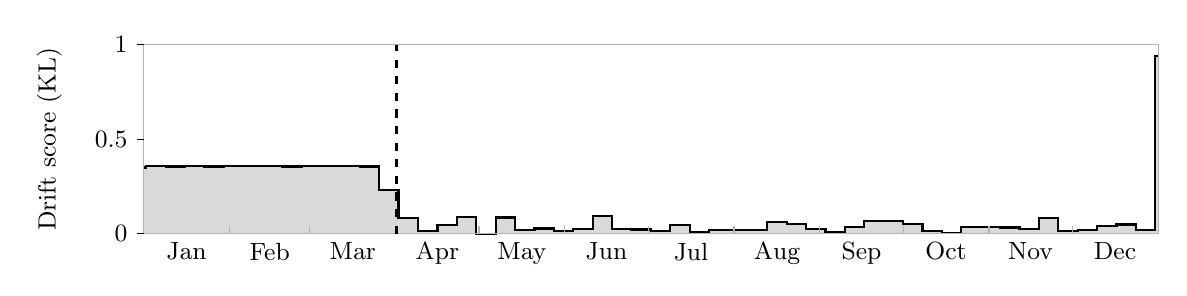
\begin{tikzpicture}[font=\small, x=0.0352cm, y=2.4000cm]
	\fill[black!15] (0.00, 0) -- (0.00, 0.3519) -- (1.00, 0.3519) -- (1.00, 0.3597) -- (8.00, 0.3597) -- (8.00, 0.3572) -- (15.00, 0.3572) -- (15.00, 0.3587) -- (22.00, 0.3587) -- (22.00, 0.3565) -- (29.00, 0.3565) -- (29.00, 0.3591) -- (36.00, 0.3591) -- (36.00, 0.3575) -- (43.00, 0.3575) -- (43.00, 0.3580) -- (50.00, 0.3580) -- (50.00, 0.3568) -- (57.00, 0.3568) -- (57.00, 0.3584) -- (64.00, 0.3584) -- (64.00, 0.3580) -- (71.00, 0.3580) -- (71.00, 0.3581) -- (78.00, 0.3581) -- (78.00, 0.3567) -- (85.00, 0.3567) -- (85.00, 0.2318) -- (92.00, 0.2318) -- (92.00, 0.0822) -- (99.00, 0.0822) -- (99.00, 0.0160) -- (106.00, 0.0160) -- (106.00, 0.0452) -- (113.00, 0.0452) -- (113.00, 0.0911) -- (120.00, 0.0911) -- (120.00, 0.0006) -- (127.00, 0.0006) -- (127.00, 0.0865) -- (134.00, 0.0865) -- (134.00, 0.0192) -- (141.00, 0.0192) -- (141.00, 0.0288) -- (148.00, 0.0288) -- (148.00, 0.0136) -- (155.00, 0.0136) -- (155.00, 0.0241) -- (162.00, 0.0241) -- (162.00, 0.0963) -- (169.00, 0.0963) -- (169.00, 0.0269) -- (176.00, 0.0269) -- (176.00, 0.0227) -- (183.00, 0.0227) -- (183.00, 0.0169) -- (190.00, 0.0169) -- (190.00, 0.0451) -- (197.00, 0.0451) -- (197.00, 0.0100) -- (204.00, 0.0100) -- (204.00, 0.0223) -- (211.00, 0.0223) -- (211.00, 0.0201) -- (218.00, 0.0201) -- (218.00, 0.0186) -- (225.00, 0.0186) -- (225.00, 0.0622) -- (232.00, 0.0622) -- (232.00, 0.0515) -- (239.00, 0.0515) -- (239.00, 0.0264) -- (246.00, 0.0264) -- (246.00, 0.0088) -- (253.00, 0.0088) -- (253.00, 0.0348) -- (260.00, 0.0348) -- (260.00, 0.0675) -- (267.00, 0.0675) -- (267.00, 0.0671) -- (274.00, 0.0671) -- (274.00, 0.0503) -- (281.00, 0.0503) -- (281.00, 0.0153) -- (288.00, 0.0153) -- (288.00, 0.0056) -- (295.00, 0.0056) -- (295.00, 0.0376) -- (302.00, 0.0376) -- (302.00, 0.0353) -- (309.00, 0.0353) -- (309.00, 0.0342) -- (316.00, 0.0342) -- (316.00, 0.0267) -- (323.00, 0.0267) -- (323.00, 0.0844) -- (330.00, 0.0844) -- (330.00, 0.0144) -- (337.00, 0.0144) -- (337.00, 0.0194) -- (344.00, 0.0194) -- (344.00, 0.0430) -- (351.00, 0.0430) -- (351.00, 0.0502) -- (358.00, 0.0502) -- (358.00, 0.0220) -- (365.00, 0.0220) -- (365.00, 0.9429) -- (366.00, 0.9429) -- (366.00, 0) -- cycle;
	\draw[thick] (0.00, 0.3519) -- (1.00, 0.3519) -- (1.00, 0.3597) -- (8.00, 0.3597) -- (8.00, 0.3572) -- (15.00, 0.3572) -- (15.00, 0.3587) -- (22.00, 0.3587) -- (22.00, 0.3565) -- (29.00, 0.3565) -- (29.00, 0.3591) -- (36.00, 0.3591) -- (36.00, 0.3575) -- (43.00, 0.3575) -- (43.00, 0.3580) -- (50.00, 0.3580) -- (50.00, 0.3568) -- (57.00, 0.3568) -- (57.00, 0.3584) -- (64.00, 0.3584) -- (64.00, 0.3580) -- (71.00, 0.3580) -- (71.00, 0.3581) -- (78.00, 0.3581) -- (78.00, 0.3567) -- (85.00, 0.3567) -- (85.00, 0.2318) -- (92.00, 0.2318) -- (92.00, 0.0822) -- (99.00, 0.0822) -- (99.00, 0.0160) -- (106.00, 0.0160) -- (106.00, 0.0452) -- (113.00, 0.0452) -- (113.00, 0.0911) -- (120.00, 0.0911) -- (120.00, 0.0006) -- (127.00, 0.0006) -- (127.00, 0.0865) -- (134.00, 0.0865) -- (134.00, 0.0192) -- (141.00, 0.0192) -- (141.00, 0.0288) -- (148.00, 0.0288) -- (148.00, 0.0136) -- (155.00, 0.0136) -- (155.00, 0.0241) -- (162.00, 0.0241) -- (162.00, 0.0963) -- (169.00, 0.0963) -- (169.00, 0.0269) -- (176.00, 0.0269) -- (176.00, 0.0227) -- (183.00, 0.0227) -- (183.00, 0.0169) -- (190.00, 0.0169) -- (190.00, 0.0451) -- (197.00, 0.0451) -- (197.00, 0.0100) -- (204.00, 0.0100) -- (204.00, 0.0223) -- (211.00, 0.0223) -- (211.00, 0.0201) -- (218.00, 0.0201) -- (218.00, 0.0186) -- (225.00, 0.0186) -- (225.00, 0.0622) -- (232.00, 0.0622) -- (232.00, 0.0515) -- (239.00, 0.0515) -- (239.00, 0.0264) -- (246.00, 0.0264) -- (246.00, 0.0088) -- (253.00, 0.0088) -- (253.00, 0.0348) -- (260.00, 0.0348) -- (260.00, 0.0675) -- (267.00, 0.0675) -- (267.00, 0.0671) -- (274.00, 0.0671) -- (274.00, 0.0503) -- (281.00, 0.0503) -- (281.00, 0.0153) -- (288.00, 0.0153) -- (288.00, 0.0056) -- (295.00, 0.0056) -- (295.00, 0.0376) -- (302.00, 0.0376) -- (302.00, 0.0353) -- (309.00, 0.0353) -- (309.00, 0.0342) -- (316.00, 0.0342) -- (316.00, 0.0267) -- (323.00, 0.0267) -- (323.00, 0.0844) -- (330.00, 0.0844) -- (330.00, 0.0144) -- (337.00, 0.0144) -- (337.00, 0.0194) -- (344.00, 0.0194) -- (344.00, 0.0430) -- (351.00, 0.0430) -- (351.00, 0.0502) -- (358.00, 0.0502) -- (358.00, 0.0220) -- (365.00, 0.0220) -- (365.00, 0.9429) -- (366.00, 0.9429);
	\draw[black!30] (0, 0) rectangle (366, 1);
	\node[below, inner sep=1pt] at (15.5, -0.0300) {Jan};
	\node[below, inner sep=1pt] at (45.5, -0.0300) {Feb};
	\draw[black!30] (31.0, 0) -- (31.0, 0.0400);
	\node[below, inner sep=1pt] at (75.5, -0.0300) {Mar};
	\draw[black!30] (60.0, 0) -- (60.0, 0.0400);
	\node[below, inner sep=1pt] at (106.0, -0.0300) {Apr};
	\draw[black!30] (91.0, 0) -- (91.0, 0.0400);
	\node[below, inner sep=1pt] at (136.5, -0.0300) {May};
	\draw[black!30] (121.0, 0) -- (121.0, 0.0400);
	\node[below, inner sep=1pt] at (167.0, -0.0300) {Jun};
	\draw[black!30] (152.0, 0) -- (152.0, 0.0400);
	\node[below, inner sep=1pt] at (197.5, -0.0300) {Jul};
	\draw[black!30] (182.0, 0) -- (182.0, 0.0400);
	\node[below, inner sep=1pt] at (228.5, -0.0300) {Aug};
	\draw[black!30] (213.0, 0) -- (213.0, 0.0400);
	\node[below, inner sep=1pt] at (259.0, -0.0300) {Sep};
	\draw[black!30] (244.0, 0) -- (244.0, 0.0400);
	\node[below, inner sep=1pt] at (289.5, -0.0300) {Oct};
	\draw[black!30] (274.0, 0) -- (274.0, 0.0400);
	\node[below, inner sep=1pt] at (320.0, -0.0300) {Nov};
	\draw[black!30] (305.0, 0) -- (305.0, 0.0400);
	\node[below, inner sep=1pt] at (350.5, -0.0300) {Dec};
	\draw[black!30] (335.0, 0) -- (335.0, 0.0400);
	\draw (0, 0) -- ++(-0.08cm, 0) node[left] {$0$};
	\draw (0, 0.5) -- ++(-0.08cm, 0) node[left] {$0.5$};
	\draw (0, 1) -- ++(-0.08cm, 0) node[left] {$1$};
	\node[rotate=90] at (-34, 0.5) {Drift score (KL)};
	\draw[dashed, thick] (91.25, 0) -- (91.25, 1);
\end{tikzpicture}

		\caption{Signal windows of one week, mean of all signal windows as reference}
		\label{fig:approach:drift_signal_intra_week}
	\end{subfigure}
	\caption[Intra-case drift signals of the running example]{%
		Drift signals of the intra-case states of the running example $L_3$ with the KL divergence (Example~\ref{ex:approach:drift_signal_intra}). Each step is a signal window at its drift score, cut at the bounds of the year 2020. The dashed line marks the control-flow drift on April~1, 2020, 06:00.
		\subref{fig:approach:drift_signal_intra_day}~The first seven signal windows have no reference. The drift gets the highest drift score of 3.47.
		\subref{fig:approach:drift_signal_intra_week}~The signal windows before the drift lie far from the mean of all signal windows and those after it close to it, so the drift shows as a step. The last signal window only holds the three events of December~31.}
	\label{fig:approach:drift_signal_intra}
\end{figure}

\begin{example}
	\label{ex:approach:drift_signal_intra}
	We compute two drift signals of the intra-case states of $L_3$ (Example~\ref{ex:approach:clustering_intra}) with the KL divergence (Figure~\ref{fig:approach:drift_signal_intra}).
	\begin{itemize}
		\item First, we choose signal windows of one day and the mean of the seven previous signal windows as reference. The 366 signal windows hold 66 events in the median.

		\item Before the drift, all drift scores are at most 0.013. On April~1, the drift score reaches its highest value 3.47, since the four new cells of the SOM (Figure~\ref{fig:approach:som_intra}) do not occur in the reference.

		\item With the previous signal window as reference, July~19 (7.98) and May~2 (5.52) exceed the drift. On July~18, all five cases execute $c$ before $b$, and on May~1, all eight cases execute $b$ before $c$. Thus, the cells of the other order are missing in the reference of the next day.

		\item Second, we choose signal windows of one week and the mean of all signal windows as reference. Before the drift, the drift scores lie between 0.35 and 0.36, and after it, their median is 0.028.

		\item Since 40 of the 54 signal windows lie after the drift, the reference is close to the new process version. Thus, the drift shows as a step downwards.
	\end{itemize}
\end{example}

\subsection{Resource Perspective}
\label{sec:approach:drift_signals:resource}
In the resource perspective, the rows are feature windows. Thus, a signal window holds far fewer rows than in the intra-case perspective. If $\Delta_s = \Delta_f$, each signal window holds exactly one feature window. Then, the drift signal with the previous signal window as reference shows exactly the state changes in the trajectory of the event log.

\begin{figure}[tb]
	\centering
	\begin{subfigure}{\textwidth}
		\centering
		% generated by notebooks/thesis, do not edit by hand
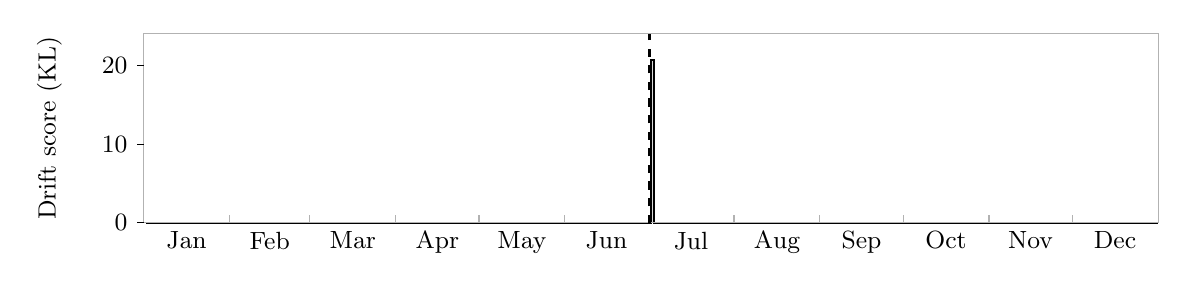
\begin{tikzpicture}[font=\small, x=0.0352cm, y=0.1000cm]
	\fill[black!15] (1.00, 0) -- (1.00, 0.0000) -- (2.00, 0.0000) -- (2.00, 0.0000) -- (3.00, 0.0000) -- (3.00, 0.0000) -- (4.00, 0.0000) -- (4.00, 0.0000) -- (5.00, 0.0000) -- (5.00, 0.0000) -- (6.00, 0.0000) -- (6.00, 0.0000) -- (7.00, 0.0000) -- (7.00, 0.0000) -- (8.00, 0.0000) -- (8.00, 0.0000) -- (9.00, 0.0000) -- (9.00, 0.0000) -- (10.00, 0.0000) -- (10.00, 0.0000) -- (11.00, 0.0000) -- (11.00, 0.0000) -- (12.00, 0.0000) -- (12.00, 0.0000) -- (13.00, 0.0000) -- (13.00, 0.0000) -- (14.00, 0.0000) -- (14.00, 0.0000) -- (15.00, 0.0000) -- (15.00, 0.0000) -- (16.00, 0.0000) -- (16.00, 0.0000) -- (17.00, 0.0000) -- (17.00, 0.0000) -- (18.00, 0.0000) -- (18.00, 0.0000) -- (19.00, 0.0000) -- (19.00, 0.0000) -- (20.00, 0.0000) -- (20.00, 0.0000) -- (21.00, 0.0000) -- (21.00, 0.0000) -- (22.00, 0.0000) -- (22.00, 0.0000) -- (23.00, 0.0000) -- (23.00, 0.0000) -- (24.00, 0.0000) -- (24.00, 0.0000) -- (25.00, 0.0000) -- (25.00, 0.0000) -- (26.00, 0.0000) -- (26.00, 0.0000) -- (27.00, 0.0000) -- (27.00, 0.0000) -- (28.00, 0.0000) -- (28.00, 0.0000) -- (29.00, 0.0000) -- (29.00, 0.0000) -- (30.00, 0.0000) -- (30.00, 0.0000) -- (31.00, 0.0000) -- (31.00, 0.0000) -- (32.00, 0.0000) -- (32.00, 0.0000) -- (33.00, 0.0000) -- (33.00, 0.0000) -- (34.00, 0.0000) -- (34.00, 0.0000) -- (35.00, 0.0000) -- (35.00, 0.0000) -- (36.00, 0.0000) -- (36.00, 0.0000) -- (37.00, 0.0000) -- (37.00, 0.0000) -- (38.00, 0.0000) -- (38.00, 0.0000) -- (39.00, 0.0000) -- (39.00, 0.0000) -- (40.00, 0.0000) -- (40.00, 0.0000) -- (41.00, 0.0000) -- (41.00, 0.0000) -- (42.00, 0.0000) -- (42.00, 0.0000) -- (43.00, 0.0000) -- (43.00, 0.0000) -- (44.00, 0.0000) -- (44.00, 0.0000) -- (45.00, 0.0000) -- (45.00, 0.0000) -- (46.00, 0.0000) -- (46.00, 0.0000) -- (47.00, 0.0000) -- (47.00, 0.0000) -- (48.00, 0.0000) -- (48.00, 0.0000) -- (49.00, 0.0000) -- (49.00, 0.0000) -- (50.00, 0.0000) -- (50.00, 0.0000) -- (51.00, 0.0000) -- (51.00, 0.0000) -- (52.00, 0.0000) -- (52.00, 0.0000) -- (53.00, 0.0000) -- (53.00, 0.0000) -- (54.00, 0.0000) -- (54.00, 0.0000) -- (55.00, 0.0000) -- (55.00, 0.0000) -- (56.00, 0.0000) -- (56.00, 0.0000) -- (57.00, 0.0000) -- (57.00, 0.0000) -- (58.00, 0.0000) -- (58.00, 0.0000) -- (59.00, 0.0000) -- (59.00, 0.0000) -- (60.00, 0.0000) -- (60.00, 0.0000) -- (61.00, 0.0000) -- (61.00, 0.0000) -- (62.00, 0.0000) -- (62.00, 0.0000) -- (63.00, 0.0000) -- (63.00, 0.0000) -- (64.00, 0.0000) -- (64.00, 0.0000) -- (65.00, 0.0000) -- (65.00, 0.0000) -- (66.00, 0.0000) -- (66.00, 0.0000) -- (67.00, 0.0000) -- (67.00, 0.0000) -- (68.00, 0.0000) -- (68.00, 0.0000) -- (69.00, 0.0000) -- (69.00, 0.0000) -- (70.00, 0.0000) -- (70.00, 0.0000) -- (71.00, 0.0000) -- (71.00, 0.0000) -- (72.00, 0.0000) -- (72.00, 0.0000) -- (73.00, 0.0000) -- (73.00, 0.0000) -- (74.00, 0.0000) -- (74.00, 0.0000) -- (75.00, 0.0000) -- (75.00, 0.0000) -- (76.00, 0.0000) -- (76.00, 0.0000) -- (77.00, 0.0000) -- (77.00, 0.0000) -- (78.00, 0.0000) -- (78.00, 0.0000) -- (79.00, 0.0000) -- (79.00, 0.0000) -- (80.00, 0.0000) -- (80.00, 0.0000) -- (81.00, 0.0000) -- (81.00, 0.0000) -- (82.00, 0.0000) -- (82.00, 0.0000) -- (83.00, 0.0000) -- (83.00, 0.0000) -- (84.00, 0.0000) -- (84.00, 0.0000) -- (85.00, 0.0000) -- (85.00, 0.0000) -- (86.00, 0.0000) -- (86.00, 0.0000) -- (87.00, 0.0000) -- (87.00, 0.0000) -- (88.00, 0.0000) -- (88.00, 0.0000) -- (89.00, 0.0000) -- (89.00, 0.0000) -- (90.00, 0.0000) -- (90.00, 0.0000) -- (91.00, 0.0000) -- (91.00, 0.0000) -- (92.00, 0.0000) -- (92.00, 0.0000) -- (93.00, 0.0000) -- (93.00, 0.0000) -- (94.00, 0.0000) -- (94.00, 0.0000) -- (95.00, 0.0000) -- (95.00, 0.0000) -- (96.00, 0.0000) -- (96.00, 0.0000) -- (97.00, 0.0000) -- (97.00, 0.0000) -- (98.00, 0.0000) -- (98.00, 0.0000) -- (99.00, 0.0000) -- (99.00, 0.0000) -- (100.00, 0.0000) -- (100.00, 0.0000) -- (101.00, 0.0000) -- (101.00, 0.0000) -- (102.00, 0.0000) -- (102.00, 0.0000) -- (103.00, 0.0000) -- (103.00, 0.0000) -- (104.00, 0.0000) -- (104.00, 0.0000) -- (105.00, 0.0000) -- (105.00, 0.0000) -- (106.00, 0.0000) -- (106.00, 0.0000) -- (107.00, 0.0000) -- (107.00, 0.0000) -- (108.00, 0.0000) -- (108.00, 0.0000) -- (109.00, 0.0000) -- (109.00, 0.0000) -- (110.00, 0.0000) -- (110.00, 0.0000) -- (111.00, 0.0000) -- (111.00, 0.0000) -- (112.00, 0.0000) -- (112.00, 0.0000) -- (113.00, 0.0000) -- (113.00, 0.0000) -- (114.00, 0.0000) -- (114.00, 0.0000) -- (115.00, 0.0000) -- (115.00, 0.0000) -- (116.00, 0.0000) -- (116.00, 0.0000) -- (117.00, 0.0000) -- (117.00, 0.0000) -- (118.00, 0.0000) -- (118.00, 0.0000) -- (119.00, 0.0000) -- (119.00, 0.0000) -- (120.00, 0.0000) -- (120.00, 0.0000) -- (121.00, 0.0000) -- (121.00, 0.0000) -- (122.00, 0.0000) -- (122.00, 0.0000) -- (123.00, 0.0000) -- (123.00, 0.0000) -- (124.00, 0.0000) -- (124.00, 0.0000) -- (125.00, 0.0000) -- (125.00, 0.0000) -- (126.00, 0.0000) -- (126.00, 0.0000) -- (127.00, 0.0000) -- (127.00, 0.0000) -- (128.00, 0.0000) -- (128.00, 0.0000) -- (129.00, 0.0000) -- (129.00, 0.0000) -- (130.00, 0.0000) -- (130.00, 0.0000) -- (131.00, 0.0000) -- (131.00, 0.0000) -- (132.00, 0.0000) -- (132.00, 0.0000) -- (133.00, 0.0000) -- (133.00, 0.0000) -- (134.00, 0.0000) -- (134.00, 0.0000) -- (135.00, 0.0000) -- (135.00, 0.0000) -- (136.00, 0.0000) -- (136.00, 0.0000) -- (137.00, 0.0000) -- (137.00, 0.0000) -- (138.00, 0.0000) -- (138.00, 0.0000) -- (139.00, 0.0000) -- (139.00, 0.0000) -- (140.00, 0.0000) -- (140.00, 0.0000) -- (141.00, 0.0000) -- (141.00, 0.0000) -- (142.00, 0.0000) -- (142.00, 0.0000) -- (143.00, 0.0000) -- (143.00, 0.0000) -- (144.00, 0.0000) -- (144.00, 0.0000) -- (145.00, 0.0000) -- (145.00, 0.0000) -- (146.00, 0.0000) -- (146.00, 0.0000) -- (147.00, 0.0000) -- (147.00, 0.0000) -- (148.00, 0.0000) -- (148.00, 0.0000) -- (149.00, 0.0000) -- (149.00, 0.0000) -- (150.00, 0.0000) -- (150.00, 0.0000) -- (151.00, 0.0000) -- (151.00, 0.0000) -- (152.00, 0.0000) -- (152.00, 0.0000) -- (153.00, 0.0000) -- (153.00, 0.0000) -- (154.00, 0.0000) -- (154.00, 0.0000) -- (155.00, 0.0000) -- (155.00, 0.0000) -- (156.00, 0.0000) -- (156.00, 0.0000) -- (157.00, 0.0000) -- (157.00, 0.0000) -- (158.00, 0.0000) -- (158.00, 0.0000) -- (159.00, 0.0000) -- (159.00, 0.0000) -- (160.00, 0.0000) -- (160.00, 0.0000) -- (161.00, 0.0000) -- (161.00, 0.0000) -- (162.00, 0.0000) -- (162.00, 0.0000) -- (163.00, 0.0000) -- (163.00, 0.0000) -- (164.00, 0.0000) -- (164.00, 0.0000) -- (165.00, 0.0000) -- (165.00, 0.0000) -- (166.00, 0.0000) -- (166.00, 0.0000) -- (167.00, 0.0000) -- (167.00, 0.0000) -- (168.00, 0.0000) -- (168.00, 0.0000) -- (169.00, 0.0000) -- (169.00, 0.0000) -- (170.00, 0.0000) -- (170.00, 0.0000) -- (171.00, 0.0000) -- (171.00, 0.0000) -- (172.00, 0.0000) -- (172.00, 0.0000) -- (173.00, 0.0000) -- (173.00, 0.0000) -- (174.00, 0.0000) -- (174.00, 0.0000) -- (175.00, 0.0000) -- (175.00, 0.0000) -- (176.00, 0.0000) -- (176.00, 0.0000) -- (177.00, 0.0000) -- (177.00, 0.0000) -- (178.00, 0.0000) -- (178.00, 0.0000) -- (179.00, 0.0000) -- (179.00, 0.0000) -- (180.00, 0.0000) -- (180.00, 0.0000) -- (181.00, 0.0000) -- (181.00, 0.0000) -- (182.00, 0.0000) -- (182.00, 0.0000) -- (183.00, 0.0000) -- (183.00, 20.7233) -- (184.00, 20.7233) -- (184.00, 0.0000) -- (185.00, 0.0000) -- (185.00, 0.0000) -- (186.00, 0.0000) -- (186.00, 0.0000) -- (187.00, 0.0000) -- (187.00, 0.0000) -- (188.00, 0.0000) -- (188.00, 0.0000) -- (189.00, 0.0000) -- (189.00, 0.0000) -- (190.00, 0.0000) -- (190.00, 0.0000) -- (191.00, 0.0000) -- (191.00, 0.0000) -- (192.00, 0.0000) -- (192.00, 0.0000) -- (193.00, 0.0000) -- (193.00, 0.0000) -- (194.00, 0.0000) -- (194.00, 0.0000) -- (195.00, 0.0000) -- (195.00, 0.0000) -- (196.00, 0.0000) -- (196.00, 0.0000) -- (197.00, 0.0000) -- (197.00, 0.0000) -- (198.00, 0.0000) -- (198.00, 0.0000) -- (199.00, 0.0000) -- (199.00, 0.0000) -- (200.00, 0.0000) -- (200.00, 0.0000) -- (201.00, 0.0000) -- (201.00, 0.0000) -- (202.00, 0.0000) -- (202.00, 0.0000) -- (203.00, 0.0000) -- (203.00, 0.0000) -- (204.00, 0.0000) -- (204.00, 0.0000) -- (205.00, 0.0000) -- (205.00, 0.0000) -- (206.00, 0.0000) -- (206.00, 0.0000) -- (207.00, 0.0000) -- (207.00, 0.0000) -- (208.00, 0.0000) -- (208.00, 0.0000) -- (209.00, 0.0000) -- (209.00, 0.0000) -- (210.00, 0.0000) -- (210.00, 0.0000) -- (211.00, 0.0000) -- (211.00, 0.0000) -- (212.00, 0.0000) -- (212.00, 0.0000) -- (213.00, 0.0000) -- (213.00, 0.0000) -- (214.00, 0.0000) -- (214.00, 0.0000) -- (215.00, 0.0000) -- (215.00, 0.0000) -- (216.00, 0.0000) -- (216.00, 0.0000) -- (217.00, 0.0000) -- (217.00, 0.0000) -- (218.00, 0.0000) -- (218.00, 0.0000) -- (219.00, 0.0000) -- (219.00, 0.0000) -- (220.00, 0.0000) -- (220.00, 0.0000) -- (221.00, 0.0000) -- (221.00, 0.0000) -- (222.00, 0.0000) -- (222.00, 0.0000) -- (223.00, 0.0000) -- (223.00, 0.0000) -- (224.00, 0.0000) -- (224.00, 0.0000) -- (225.00, 0.0000) -- (225.00, 0.0000) -- (226.00, 0.0000) -- (226.00, 0.0000) -- (227.00, 0.0000) -- (227.00, 0.0000) -- (228.00, 0.0000) -- (228.00, 0.0000) -- (229.00, 0.0000) -- (229.00, 0.0000) -- (230.00, 0.0000) -- (230.00, 0.0000) -- (231.00, 0.0000) -- (231.00, 0.0000) -- (232.00, 0.0000) -- (232.00, 0.0000) -- (233.00, 0.0000) -- (233.00, 0.0000) -- (234.00, 0.0000) -- (234.00, 0.0000) -- (235.00, 0.0000) -- (235.00, 0.0000) -- (236.00, 0.0000) -- (236.00, 0.0000) -- (237.00, 0.0000) -- (237.00, 0.0000) -- (238.00, 0.0000) -- (238.00, 0.0000) -- (239.00, 0.0000) -- (239.00, 0.0000) -- (240.00, 0.0000) -- (240.00, 0.0000) -- (241.00, 0.0000) -- (241.00, 0.0000) -- (242.00, 0.0000) -- (242.00, 0.0000) -- (243.00, 0.0000) -- (243.00, 0.0000) -- (244.00, 0.0000) -- (244.00, 0.0000) -- (245.00, 0.0000) -- (245.00, 0.0000) -- (246.00, 0.0000) -- (246.00, 0.0000) -- (247.00, 0.0000) -- (247.00, 0.0000) -- (248.00, 0.0000) -- (248.00, 0.0000) -- (249.00, 0.0000) -- (249.00, 0.0000) -- (250.00, 0.0000) -- (250.00, 0.0000) -- (251.00, 0.0000) -- (251.00, 0.0000) -- (252.00, 0.0000) -- (252.00, 0.0000) -- (253.00, 0.0000) -- (253.00, 0.0000) -- (254.00, 0.0000) -- (254.00, 0.0000) -- (255.00, 0.0000) -- (255.00, 0.0000) -- (256.00, 0.0000) -- (256.00, 0.0000) -- (257.00, 0.0000) -- (257.00, 0.0000) -- (258.00, 0.0000) -- (258.00, 0.0000) -- (259.00, 0.0000) -- (259.00, 0.0000) -- (260.00, 0.0000) -- (260.00, 0.0000) -- (261.00, 0.0000) -- (261.00, 0.0000) -- (262.00, 0.0000) -- (262.00, 0.0000) -- (263.00, 0.0000) -- (263.00, 0.0000) -- (264.00, 0.0000) -- (264.00, 0.0000) -- (265.00, 0.0000) -- (265.00, 0.0000) -- (266.00, 0.0000) -- (266.00, 0.0000) -- (267.00, 0.0000) -- (267.00, 0.0000) -- (268.00, 0.0000) -- (268.00, 0.0000) -- (269.00, 0.0000) -- (269.00, 0.0000) -- (270.00, 0.0000) -- (270.00, 0.0000) -- (271.00, 0.0000) -- (271.00, 0.0000) -- (272.00, 0.0000) -- (272.00, 0.0000) -- (273.00, 0.0000) -- (273.00, 0.0000) -- (274.00, 0.0000) -- (274.00, 0.0000) -- (275.00, 0.0000) -- (275.00, 0.0000) -- (276.00, 0.0000) -- (276.00, 0.0000) -- (277.00, 0.0000) -- (277.00, 0.0000) -- (278.00, 0.0000) -- (278.00, 0.0000) -- (279.00, 0.0000) -- (279.00, 0.0000) -- (280.00, 0.0000) -- (280.00, 0.0000) -- (281.00, 0.0000) -- (281.00, 0.0000) -- (282.00, 0.0000) -- (282.00, 0.0000) -- (283.00, 0.0000) -- (283.00, 0.0000) -- (284.00, 0.0000) -- (284.00, 0.0000) -- (285.00, 0.0000) -- (285.00, 0.0000) -- (286.00, 0.0000) -- (286.00, 0.0000) -- (287.00, 0.0000) -- (287.00, 0.0000) -- (288.00, 0.0000) -- (288.00, 0.0000) -- (289.00, 0.0000) -- (289.00, 0.0000) -- (290.00, 0.0000) -- (290.00, 0.0000) -- (291.00, 0.0000) -- (291.00, 0.0000) -- (292.00, 0.0000) -- (292.00, 0.0000) -- (293.00, 0.0000) -- (293.00, 0.0000) -- (294.00, 0.0000) -- (294.00, 0.0000) -- (295.00, 0.0000) -- (295.00, 0.0000) -- (296.00, 0.0000) -- (296.00, 0.0000) -- (297.00, 0.0000) -- (297.00, 0.0000) -- (298.00, 0.0000) -- (298.00, 0.0000) -- (299.00, 0.0000) -- (299.00, 0.0000) -- (300.00, 0.0000) -- (300.00, 0.0000) -- (301.00, 0.0000) -- (301.00, 0.0000) -- (302.00, 0.0000) -- (302.00, 0.0000) -- (303.00, 0.0000) -- (303.00, 0.0000) -- (304.00, 0.0000) -- (304.00, 0.0000) -- (305.00, 0.0000) -- (305.00, 0.0000) -- (306.00, 0.0000) -- (306.00, 0.0000) -- (307.00, 0.0000) -- (307.00, 0.0000) -- (308.00, 0.0000) -- (308.00, 0.0000) -- (309.00, 0.0000) -- (309.00, 0.0000) -- (310.00, 0.0000) -- (310.00, 0.0000) -- (311.00, 0.0000) -- (311.00, 0.0000) -- (312.00, 0.0000) -- (312.00, 0.0000) -- (313.00, 0.0000) -- (313.00, 0.0000) -- (314.00, 0.0000) -- (314.00, 0.0000) -- (315.00, 0.0000) -- (315.00, 0.0000) -- (316.00, 0.0000) -- (316.00, 0.0000) -- (317.00, 0.0000) -- (317.00, 0.0000) -- (318.00, 0.0000) -- (318.00, 0.0000) -- (319.00, 0.0000) -- (319.00, 0.0000) -- (320.00, 0.0000) -- (320.00, 0.0000) -- (321.00, 0.0000) -- (321.00, 0.0000) -- (322.00, 0.0000) -- (322.00, 0.0000) -- (323.00, 0.0000) -- (323.00, 0.0000) -- (324.00, 0.0000) -- (324.00, 0.0000) -- (325.00, 0.0000) -- (325.00, 0.0000) -- (326.00, 0.0000) -- (326.00, 0.0000) -- (327.00, 0.0000) -- (327.00, 0.0000) -- (328.00, 0.0000) -- (328.00, 0.0000) -- (329.00, 0.0000) -- (329.00, 0.0000) -- (330.00, 0.0000) -- (330.00, 0.0000) -- (331.00, 0.0000) -- (331.00, 0.0000) -- (332.00, 0.0000) -- (332.00, 0.0000) -- (333.00, 0.0000) -- (333.00, 0.0000) -- (334.00, 0.0000) -- (334.00, 0.0000) -- (335.00, 0.0000) -- (335.00, 0.0000) -- (336.00, 0.0000) -- (336.00, 0.0000) -- (337.00, 0.0000) -- (337.00, 0.0000) -- (338.00, 0.0000) -- (338.00, 0.0000) -- (339.00, 0.0000) -- (339.00, 0.0000) -- (340.00, 0.0000) -- (340.00, 0.0000) -- (341.00, 0.0000) -- (341.00, 0.0000) -- (342.00, 0.0000) -- (342.00, 0.0000) -- (343.00, 0.0000) -- (343.00, 0.0000) -- (344.00, 0.0000) -- (344.00, 0.0000) -- (345.00, 0.0000) -- (345.00, 0.0000) -- (346.00, 0.0000) -- (346.00, 0.0000) -- (347.00, 0.0000) -- (347.00, 0.0000) -- (348.00, 0.0000) -- (348.00, 0.0000) -- (349.00, 0.0000) -- (349.00, 0.0000) -- (350.00, 0.0000) -- (350.00, 0.0000) -- (351.00, 0.0000) -- (351.00, 0.0000) -- (352.00, 0.0000) -- (352.00, 0.0000) -- (353.00, 0.0000) -- (353.00, 0.0000) -- (354.00, 0.0000) -- (354.00, 0.0000) -- (355.00, 0.0000) -- (355.00, 0.0000) -- (356.00, 0.0000) -- (356.00, 0.0000) -- (357.00, 0.0000) -- (357.00, 0.0000) -- (358.00, 0.0000) -- (358.00, 0.0000) -- (359.00, 0.0000) -- (359.00, 0.0000) -- (360.00, 0.0000) -- (360.00, 0.0000) -- (361.00, 0.0000) -- (361.00, 0.0000) -- (362.00, 0.0000) -- (362.00, 0.0000) -- (363.00, 0.0000) -- (363.00, 0.0000) -- (364.00, 0.0000) -- (364.00, 0.0000) -- (365.00, 0.0000) -- (365.00, 0.0000) -- (366.00, 0.0000) -- (366.00, 0) -- cycle;
	\draw[thick] (1.00, 0.0000) -- (2.00, 0.0000) -- (2.00, 0.0000) -- (3.00, 0.0000) -- (3.00, 0.0000) -- (4.00, 0.0000) -- (4.00, 0.0000) -- (5.00, 0.0000) -- (5.00, 0.0000) -- (6.00, 0.0000) -- (6.00, 0.0000) -- (7.00, 0.0000) -- (7.00, 0.0000) -- (8.00, 0.0000) -- (8.00, 0.0000) -- (9.00, 0.0000) -- (9.00, 0.0000) -- (10.00, 0.0000) -- (10.00, 0.0000) -- (11.00, 0.0000) -- (11.00, 0.0000) -- (12.00, 0.0000) -- (12.00, 0.0000) -- (13.00, 0.0000) -- (13.00, 0.0000) -- (14.00, 0.0000) -- (14.00, 0.0000) -- (15.00, 0.0000) -- (15.00, 0.0000) -- (16.00, 0.0000) -- (16.00, 0.0000) -- (17.00, 0.0000) -- (17.00, 0.0000) -- (18.00, 0.0000) -- (18.00, 0.0000) -- (19.00, 0.0000) -- (19.00, 0.0000) -- (20.00, 0.0000) -- (20.00, 0.0000) -- (21.00, 0.0000) -- (21.00, 0.0000) -- (22.00, 0.0000) -- (22.00, 0.0000) -- (23.00, 0.0000) -- (23.00, 0.0000) -- (24.00, 0.0000) -- (24.00, 0.0000) -- (25.00, 0.0000) -- (25.00, 0.0000) -- (26.00, 0.0000) -- (26.00, 0.0000) -- (27.00, 0.0000) -- (27.00, 0.0000) -- (28.00, 0.0000) -- (28.00, 0.0000) -- (29.00, 0.0000) -- (29.00, 0.0000) -- (30.00, 0.0000) -- (30.00, 0.0000) -- (31.00, 0.0000) -- (31.00, 0.0000) -- (32.00, 0.0000) -- (32.00, 0.0000) -- (33.00, 0.0000) -- (33.00, 0.0000) -- (34.00, 0.0000) -- (34.00, 0.0000) -- (35.00, 0.0000) -- (35.00, 0.0000) -- (36.00, 0.0000) -- (36.00, 0.0000) -- (37.00, 0.0000) -- (37.00, 0.0000) -- (38.00, 0.0000) -- (38.00, 0.0000) -- (39.00, 0.0000) -- (39.00, 0.0000) -- (40.00, 0.0000) -- (40.00, 0.0000) -- (41.00, 0.0000) -- (41.00, 0.0000) -- (42.00, 0.0000) -- (42.00, 0.0000) -- (43.00, 0.0000) -- (43.00, 0.0000) -- (44.00, 0.0000) -- (44.00, 0.0000) -- (45.00, 0.0000) -- (45.00, 0.0000) -- (46.00, 0.0000) -- (46.00, 0.0000) -- (47.00, 0.0000) -- (47.00, 0.0000) -- (48.00, 0.0000) -- (48.00, 0.0000) -- (49.00, 0.0000) -- (49.00, 0.0000) -- (50.00, 0.0000) -- (50.00, 0.0000) -- (51.00, 0.0000) -- (51.00, 0.0000) -- (52.00, 0.0000) -- (52.00, 0.0000) -- (53.00, 0.0000) -- (53.00, 0.0000) -- (54.00, 0.0000) -- (54.00, 0.0000) -- (55.00, 0.0000) -- (55.00, 0.0000) -- (56.00, 0.0000) -- (56.00, 0.0000) -- (57.00, 0.0000) -- (57.00, 0.0000) -- (58.00, 0.0000) -- (58.00, 0.0000) -- (59.00, 0.0000) -- (59.00, 0.0000) -- (60.00, 0.0000) -- (60.00, 0.0000) -- (61.00, 0.0000) -- (61.00, 0.0000) -- (62.00, 0.0000) -- (62.00, 0.0000) -- (63.00, 0.0000) -- (63.00, 0.0000) -- (64.00, 0.0000) -- (64.00, 0.0000) -- (65.00, 0.0000) -- (65.00, 0.0000) -- (66.00, 0.0000) -- (66.00, 0.0000) -- (67.00, 0.0000) -- (67.00, 0.0000) -- (68.00, 0.0000) -- (68.00, 0.0000) -- (69.00, 0.0000) -- (69.00, 0.0000) -- (70.00, 0.0000) -- (70.00, 0.0000) -- (71.00, 0.0000) -- (71.00, 0.0000) -- (72.00, 0.0000) -- (72.00, 0.0000) -- (73.00, 0.0000) -- (73.00, 0.0000) -- (74.00, 0.0000) -- (74.00, 0.0000) -- (75.00, 0.0000) -- (75.00, 0.0000) -- (76.00, 0.0000) -- (76.00, 0.0000) -- (77.00, 0.0000) -- (77.00, 0.0000) -- (78.00, 0.0000) -- (78.00, 0.0000) -- (79.00, 0.0000) -- (79.00, 0.0000) -- (80.00, 0.0000) -- (80.00, 0.0000) -- (81.00, 0.0000) -- (81.00, 0.0000) -- (82.00, 0.0000) -- (82.00, 0.0000) -- (83.00, 0.0000) -- (83.00, 0.0000) -- (84.00, 0.0000) -- (84.00, 0.0000) -- (85.00, 0.0000) -- (85.00, 0.0000) -- (86.00, 0.0000) -- (86.00, 0.0000) -- (87.00, 0.0000) -- (87.00, 0.0000) -- (88.00, 0.0000) -- (88.00, 0.0000) -- (89.00, 0.0000) -- (89.00, 0.0000) -- (90.00, 0.0000) -- (90.00, 0.0000) -- (91.00, 0.0000) -- (91.00, 0.0000) -- (92.00, 0.0000) -- (92.00, 0.0000) -- (93.00, 0.0000) -- (93.00, 0.0000) -- (94.00, 0.0000) -- (94.00, 0.0000) -- (95.00, 0.0000) -- (95.00, 0.0000) -- (96.00, 0.0000) -- (96.00, 0.0000) -- (97.00, 0.0000) -- (97.00, 0.0000) -- (98.00, 0.0000) -- (98.00, 0.0000) -- (99.00, 0.0000) -- (99.00, 0.0000) -- (100.00, 0.0000) -- (100.00, 0.0000) -- (101.00, 0.0000) -- (101.00, 0.0000) -- (102.00, 0.0000) -- (102.00, 0.0000) -- (103.00, 0.0000) -- (103.00, 0.0000) -- (104.00, 0.0000) -- (104.00, 0.0000) -- (105.00, 0.0000) -- (105.00, 0.0000) -- (106.00, 0.0000) -- (106.00, 0.0000) -- (107.00, 0.0000) -- (107.00, 0.0000) -- (108.00, 0.0000) -- (108.00, 0.0000) -- (109.00, 0.0000) -- (109.00, 0.0000) -- (110.00, 0.0000) -- (110.00, 0.0000) -- (111.00, 0.0000) -- (111.00, 0.0000) -- (112.00, 0.0000) -- (112.00, 0.0000) -- (113.00, 0.0000) -- (113.00, 0.0000) -- (114.00, 0.0000) -- (114.00, 0.0000) -- (115.00, 0.0000) -- (115.00, 0.0000) -- (116.00, 0.0000) -- (116.00, 0.0000) -- (117.00, 0.0000) -- (117.00, 0.0000) -- (118.00, 0.0000) -- (118.00, 0.0000) -- (119.00, 0.0000) -- (119.00, 0.0000) -- (120.00, 0.0000) -- (120.00, 0.0000) -- (121.00, 0.0000) -- (121.00, 0.0000) -- (122.00, 0.0000) -- (122.00, 0.0000) -- (123.00, 0.0000) -- (123.00, 0.0000) -- (124.00, 0.0000) -- (124.00, 0.0000) -- (125.00, 0.0000) -- (125.00, 0.0000) -- (126.00, 0.0000) -- (126.00, 0.0000) -- (127.00, 0.0000) -- (127.00, 0.0000) -- (128.00, 0.0000) -- (128.00, 0.0000) -- (129.00, 0.0000) -- (129.00, 0.0000) -- (130.00, 0.0000) -- (130.00, 0.0000) -- (131.00, 0.0000) -- (131.00, 0.0000) -- (132.00, 0.0000) -- (132.00, 0.0000) -- (133.00, 0.0000) -- (133.00, 0.0000) -- (134.00, 0.0000) -- (134.00, 0.0000) -- (135.00, 0.0000) -- (135.00, 0.0000) -- (136.00, 0.0000) -- (136.00, 0.0000) -- (137.00, 0.0000) -- (137.00, 0.0000) -- (138.00, 0.0000) -- (138.00, 0.0000) -- (139.00, 0.0000) -- (139.00, 0.0000) -- (140.00, 0.0000) -- (140.00, 0.0000) -- (141.00, 0.0000) -- (141.00, 0.0000) -- (142.00, 0.0000) -- (142.00, 0.0000) -- (143.00, 0.0000) -- (143.00, 0.0000) -- (144.00, 0.0000) -- (144.00, 0.0000) -- (145.00, 0.0000) -- (145.00, 0.0000) -- (146.00, 0.0000) -- (146.00, 0.0000) -- (147.00, 0.0000) -- (147.00, 0.0000) -- (148.00, 0.0000) -- (148.00, 0.0000) -- (149.00, 0.0000) -- (149.00, 0.0000) -- (150.00, 0.0000) -- (150.00, 0.0000) -- (151.00, 0.0000) -- (151.00, 0.0000) -- (152.00, 0.0000) -- (152.00, 0.0000) -- (153.00, 0.0000) -- (153.00, 0.0000) -- (154.00, 0.0000) -- (154.00, 0.0000) -- (155.00, 0.0000) -- (155.00, 0.0000) -- (156.00, 0.0000) -- (156.00, 0.0000) -- (157.00, 0.0000) -- (157.00, 0.0000) -- (158.00, 0.0000) -- (158.00, 0.0000) -- (159.00, 0.0000) -- (159.00, 0.0000) -- (160.00, 0.0000) -- (160.00, 0.0000) -- (161.00, 0.0000) -- (161.00, 0.0000) -- (162.00, 0.0000) -- (162.00, 0.0000) -- (163.00, 0.0000) -- (163.00, 0.0000) -- (164.00, 0.0000) -- (164.00, 0.0000) -- (165.00, 0.0000) -- (165.00, 0.0000) -- (166.00, 0.0000) -- (166.00, 0.0000) -- (167.00, 0.0000) -- (167.00, 0.0000) -- (168.00, 0.0000) -- (168.00, 0.0000) -- (169.00, 0.0000) -- (169.00, 0.0000) -- (170.00, 0.0000) -- (170.00, 0.0000) -- (171.00, 0.0000) -- (171.00, 0.0000) -- (172.00, 0.0000) -- (172.00, 0.0000) -- (173.00, 0.0000) -- (173.00, 0.0000) -- (174.00, 0.0000) -- (174.00, 0.0000) -- (175.00, 0.0000) -- (175.00, 0.0000) -- (176.00, 0.0000) -- (176.00, 0.0000) -- (177.00, 0.0000) -- (177.00, 0.0000) -- (178.00, 0.0000) -- (178.00, 0.0000) -- (179.00, 0.0000) -- (179.00, 0.0000) -- (180.00, 0.0000) -- (180.00, 0.0000) -- (181.00, 0.0000) -- (181.00, 0.0000) -- (182.00, 0.0000) -- (182.00, 0.0000) -- (183.00, 0.0000) -- (183.00, 20.7233) -- (184.00, 20.7233) -- (184.00, 0.0000) -- (185.00, 0.0000) -- (185.00, 0.0000) -- (186.00, 0.0000) -- (186.00, 0.0000) -- (187.00, 0.0000) -- (187.00, 0.0000) -- (188.00, 0.0000) -- (188.00, 0.0000) -- (189.00, 0.0000) -- (189.00, 0.0000) -- (190.00, 0.0000) -- (190.00, 0.0000) -- (191.00, 0.0000) -- (191.00, 0.0000) -- (192.00, 0.0000) -- (192.00, 0.0000) -- (193.00, 0.0000) -- (193.00, 0.0000) -- (194.00, 0.0000) -- (194.00, 0.0000) -- (195.00, 0.0000) -- (195.00, 0.0000) -- (196.00, 0.0000) -- (196.00, 0.0000) -- (197.00, 0.0000) -- (197.00, 0.0000) -- (198.00, 0.0000) -- (198.00, 0.0000) -- (199.00, 0.0000) -- (199.00, 0.0000) -- (200.00, 0.0000) -- (200.00, 0.0000) -- (201.00, 0.0000) -- (201.00, 0.0000) -- (202.00, 0.0000) -- (202.00, 0.0000) -- (203.00, 0.0000) -- (203.00, 0.0000) -- (204.00, 0.0000) -- (204.00, 0.0000) -- (205.00, 0.0000) -- (205.00, 0.0000) -- (206.00, 0.0000) -- (206.00, 0.0000) -- (207.00, 0.0000) -- (207.00, 0.0000) -- (208.00, 0.0000) -- (208.00, 0.0000) -- (209.00, 0.0000) -- (209.00, 0.0000) -- (210.00, 0.0000) -- (210.00, 0.0000) -- (211.00, 0.0000) -- (211.00, 0.0000) -- (212.00, 0.0000) -- (212.00, 0.0000) -- (213.00, 0.0000) -- (213.00, 0.0000) -- (214.00, 0.0000) -- (214.00, 0.0000) -- (215.00, 0.0000) -- (215.00, 0.0000) -- (216.00, 0.0000) -- (216.00, 0.0000) -- (217.00, 0.0000) -- (217.00, 0.0000) -- (218.00, 0.0000) -- (218.00, 0.0000) -- (219.00, 0.0000) -- (219.00, 0.0000) -- (220.00, 0.0000) -- (220.00, 0.0000) -- (221.00, 0.0000) -- (221.00, 0.0000) -- (222.00, 0.0000) -- (222.00, 0.0000) -- (223.00, 0.0000) -- (223.00, 0.0000) -- (224.00, 0.0000) -- (224.00, 0.0000) -- (225.00, 0.0000) -- (225.00, 0.0000) -- (226.00, 0.0000) -- (226.00, 0.0000) -- (227.00, 0.0000) -- (227.00, 0.0000) -- (228.00, 0.0000) -- (228.00, 0.0000) -- (229.00, 0.0000) -- (229.00, 0.0000) -- (230.00, 0.0000) -- (230.00, 0.0000) -- (231.00, 0.0000) -- (231.00, 0.0000) -- (232.00, 0.0000) -- (232.00, 0.0000) -- (233.00, 0.0000) -- (233.00, 0.0000) -- (234.00, 0.0000) -- (234.00, 0.0000) -- (235.00, 0.0000) -- (235.00, 0.0000) -- (236.00, 0.0000) -- (236.00, 0.0000) -- (237.00, 0.0000) -- (237.00, 0.0000) -- (238.00, 0.0000) -- (238.00, 0.0000) -- (239.00, 0.0000) -- (239.00, 0.0000) -- (240.00, 0.0000) -- (240.00, 0.0000) -- (241.00, 0.0000) -- (241.00, 0.0000) -- (242.00, 0.0000) -- (242.00, 0.0000) -- (243.00, 0.0000) -- (243.00, 0.0000) -- (244.00, 0.0000) -- (244.00, 0.0000) -- (245.00, 0.0000) -- (245.00, 0.0000) -- (246.00, 0.0000) -- (246.00, 0.0000) -- (247.00, 0.0000) -- (247.00, 0.0000) -- (248.00, 0.0000) -- (248.00, 0.0000) -- (249.00, 0.0000) -- (249.00, 0.0000) -- (250.00, 0.0000) -- (250.00, 0.0000) -- (251.00, 0.0000) -- (251.00, 0.0000) -- (252.00, 0.0000) -- (252.00, 0.0000) -- (253.00, 0.0000) -- (253.00, 0.0000) -- (254.00, 0.0000) -- (254.00, 0.0000) -- (255.00, 0.0000) -- (255.00, 0.0000) -- (256.00, 0.0000) -- (256.00, 0.0000) -- (257.00, 0.0000) -- (257.00, 0.0000) -- (258.00, 0.0000) -- (258.00, 0.0000) -- (259.00, 0.0000) -- (259.00, 0.0000) -- (260.00, 0.0000) -- (260.00, 0.0000) -- (261.00, 0.0000) -- (261.00, 0.0000) -- (262.00, 0.0000) -- (262.00, 0.0000) -- (263.00, 0.0000) -- (263.00, 0.0000) -- (264.00, 0.0000) -- (264.00, 0.0000) -- (265.00, 0.0000) -- (265.00, 0.0000) -- (266.00, 0.0000) -- (266.00, 0.0000) -- (267.00, 0.0000) -- (267.00, 0.0000) -- (268.00, 0.0000) -- (268.00, 0.0000) -- (269.00, 0.0000) -- (269.00, 0.0000) -- (270.00, 0.0000) -- (270.00, 0.0000) -- (271.00, 0.0000) -- (271.00, 0.0000) -- (272.00, 0.0000) -- (272.00, 0.0000) -- (273.00, 0.0000) -- (273.00, 0.0000) -- (274.00, 0.0000) -- (274.00, 0.0000) -- (275.00, 0.0000) -- (275.00, 0.0000) -- (276.00, 0.0000) -- (276.00, 0.0000) -- (277.00, 0.0000) -- (277.00, 0.0000) -- (278.00, 0.0000) -- (278.00, 0.0000) -- (279.00, 0.0000) -- (279.00, 0.0000) -- (280.00, 0.0000) -- (280.00, 0.0000) -- (281.00, 0.0000) -- (281.00, 0.0000) -- (282.00, 0.0000) -- (282.00, 0.0000) -- (283.00, 0.0000) -- (283.00, 0.0000) -- (284.00, 0.0000) -- (284.00, 0.0000) -- (285.00, 0.0000) -- (285.00, 0.0000) -- (286.00, 0.0000) -- (286.00, 0.0000) -- (287.00, 0.0000) -- (287.00, 0.0000) -- (288.00, 0.0000) -- (288.00, 0.0000) -- (289.00, 0.0000) -- (289.00, 0.0000) -- (290.00, 0.0000) -- (290.00, 0.0000) -- (291.00, 0.0000) -- (291.00, 0.0000) -- (292.00, 0.0000) -- (292.00, 0.0000) -- (293.00, 0.0000) -- (293.00, 0.0000) -- (294.00, 0.0000) -- (294.00, 0.0000) -- (295.00, 0.0000) -- (295.00, 0.0000) -- (296.00, 0.0000) -- (296.00, 0.0000) -- (297.00, 0.0000) -- (297.00, 0.0000) -- (298.00, 0.0000) -- (298.00, 0.0000) -- (299.00, 0.0000) -- (299.00, 0.0000) -- (300.00, 0.0000) -- (300.00, 0.0000) -- (301.00, 0.0000) -- (301.00, 0.0000) -- (302.00, 0.0000) -- (302.00, 0.0000) -- (303.00, 0.0000) -- (303.00, 0.0000) -- (304.00, 0.0000) -- (304.00, 0.0000) -- (305.00, 0.0000) -- (305.00, 0.0000) -- (306.00, 0.0000) -- (306.00, 0.0000) -- (307.00, 0.0000) -- (307.00, 0.0000) -- (308.00, 0.0000) -- (308.00, 0.0000) -- (309.00, 0.0000) -- (309.00, 0.0000) -- (310.00, 0.0000) -- (310.00, 0.0000) -- (311.00, 0.0000) -- (311.00, 0.0000) -- (312.00, 0.0000) -- (312.00, 0.0000) -- (313.00, 0.0000) -- (313.00, 0.0000) -- (314.00, 0.0000) -- (314.00, 0.0000) -- (315.00, 0.0000) -- (315.00, 0.0000) -- (316.00, 0.0000) -- (316.00, 0.0000) -- (317.00, 0.0000) -- (317.00, 0.0000) -- (318.00, 0.0000) -- (318.00, 0.0000) -- (319.00, 0.0000) -- (319.00, 0.0000) -- (320.00, 0.0000) -- (320.00, 0.0000) -- (321.00, 0.0000) -- (321.00, 0.0000) -- (322.00, 0.0000) -- (322.00, 0.0000) -- (323.00, 0.0000) -- (323.00, 0.0000) -- (324.00, 0.0000) -- (324.00, 0.0000) -- (325.00, 0.0000) -- (325.00, 0.0000) -- (326.00, 0.0000) -- (326.00, 0.0000) -- (327.00, 0.0000) -- (327.00, 0.0000) -- (328.00, 0.0000) -- (328.00, 0.0000) -- (329.00, 0.0000) -- (329.00, 0.0000) -- (330.00, 0.0000) -- (330.00, 0.0000) -- (331.00, 0.0000) -- (331.00, 0.0000) -- (332.00, 0.0000) -- (332.00, 0.0000) -- (333.00, 0.0000) -- (333.00, 0.0000) -- (334.00, 0.0000) -- (334.00, 0.0000) -- (335.00, 0.0000) -- (335.00, 0.0000) -- (336.00, 0.0000) -- (336.00, 0.0000) -- (337.00, 0.0000) -- (337.00, 0.0000) -- (338.00, 0.0000) -- (338.00, 0.0000) -- (339.00, 0.0000) -- (339.00, 0.0000) -- (340.00, 0.0000) -- (340.00, 0.0000) -- (341.00, 0.0000) -- (341.00, 0.0000) -- (342.00, 0.0000) -- (342.00, 0.0000) -- (343.00, 0.0000) -- (343.00, 0.0000) -- (344.00, 0.0000) -- (344.00, 0.0000) -- (345.00, 0.0000) -- (345.00, 0.0000) -- (346.00, 0.0000) -- (346.00, 0.0000) -- (347.00, 0.0000) -- (347.00, 0.0000) -- (348.00, 0.0000) -- (348.00, 0.0000) -- (349.00, 0.0000) -- (349.00, 0.0000) -- (350.00, 0.0000) -- (350.00, 0.0000) -- (351.00, 0.0000) -- (351.00, 0.0000) -- (352.00, 0.0000) -- (352.00, 0.0000) -- (353.00, 0.0000) -- (353.00, 0.0000) -- (354.00, 0.0000) -- (354.00, 0.0000) -- (355.00, 0.0000) -- (355.00, 0.0000) -- (356.00, 0.0000) -- (356.00, 0.0000) -- (357.00, 0.0000) -- (357.00, 0.0000) -- (358.00, 0.0000) -- (358.00, 0.0000) -- (359.00, 0.0000) -- (359.00, 0.0000) -- (360.00, 0.0000) -- (360.00, 0.0000) -- (361.00, 0.0000) -- (361.00, 0.0000) -- (362.00, 0.0000) -- (362.00, 0.0000) -- (363.00, 0.0000) -- (363.00, 0.0000) -- (364.00, 0.0000) -- (364.00, 0.0000) -- (365.00, 0.0000) -- (365.00, 0.0000) -- (366.00, 0.0000);
	\draw[black!30] (0, 0) rectangle (366, 24);
	\node[below, inner sep=1pt] at (15.5, -0.7200) {Jan};
	\node[below, inner sep=1pt] at (45.5, -0.7200) {Feb};
	\draw[black!30] (31.0, 0) -- (31.0, 0.9600);
	\node[below, inner sep=1pt] at (75.5, -0.7200) {Mar};
	\draw[black!30] (60.0, 0) -- (60.0, 0.9600);
	\node[below, inner sep=1pt] at (106.0, -0.7200) {Apr};
	\draw[black!30] (91.0, 0) -- (91.0, 0.9600);
	\node[below, inner sep=1pt] at (136.5, -0.7200) {May};
	\draw[black!30] (121.0, 0) -- (121.0, 0.9600);
	\node[below, inner sep=1pt] at (167.0, -0.7200) {Jun};
	\draw[black!30] (152.0, 0) -- (152.0, 0.9600);
	\node[below, inner sep=1pt] at (197.5, -0.7200) {Jul};
	\draw[black!30] (182.0, 0) -- (182.0, 0.9600);
	\node[below, inner sep=1pt] at (228.5, -0.7200) {Aug};
	\draw[black!30] (213.0, 0) -- (213.0, 0.9600);
	\node[below, inner sep=1pt] at (259.0, -0.7200) {Sep};
	\draw[black!30] (244.0, 0) -- (244.0, 0.9600);
	\node[below, inner sep=1pt] at (289.5, -0.7200) {Oct};
	\draw[black!30] (274.0, 0) -- (274.0, 0.9600);
	\node[below, inner sep=1pt] at (320.0, -0.7200) {Nov};
	\draw[black!30] (305.0, 0) -- (305.0, 0.9600);
	\node[below, inner sep=1pt] at (350.5, -0.7200) {Dec};
	\draw[black!30] (335.0, 0) -- (335.0, 0.9600);
	\draw (0, 0) -- ++(-0.08cm, 0) node[left] {$0$};
	\draw (0, 10) -- ++(-0.08cm, 0) node[left] {$10$};
	\draw (0, 20) -- ++(-0.08cm, 0) node[left] {$20$};
	\node[rotate=90] at (-34, 12) {Drift score (KL)};
	\draw[dashed, thick] (182.50, 0) -- (182.50, 24);
\end{tikzpicture}

		\caption{Signal windows of one day, previous signal window as reference}
		\label{fig:approach:drift_signal_resource_day}
	\end{subfigure}

	\medskip
	\begin{subfigure}{\textwidth}
		\centering
		% generated by notebooks/thesis, do not edit by hand
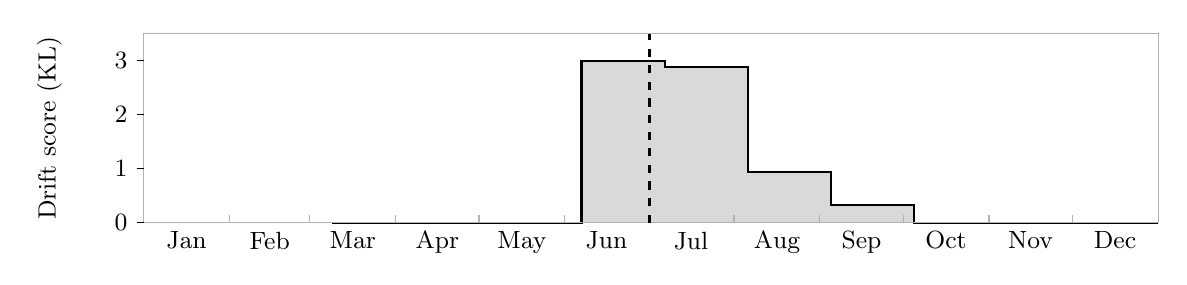
\begin{tikzpicture}[font=\small, x=0.0352cm, y=0.6857cm]
	\fill[black!15] (68.00, 0) -- (68.00, 0.0000) -- (98.00, 0.0000) -- (98.00, 0.0000) -- (128.00, 0.0000) -- (128.00, 0.0000) -- (158.00, 0.0000) -- (158.00, 3.0033) -- (188.00, 3.0033) -- (188.00, 2.8904) -- (218.00, 2.8904) -- (218.00, 0.9445) -- (248.00, 0.9445) -- (248.00, 0.3254) -- (278.00, 0.3254) -- (278.00, 0.0000) -- (308.00, 0.0000) -- (308.00, 0.0000) -- (338.00, 0.0000) -- (338.00, 0.0000) -- (366.00, 0.0000) -- (366.00, 0) -- cycle;
	\draw[thick] (68.00, 0.0000) -- (98.00, 0.0000) -- (98.00, 0.0000) -- (128.00, 0.0000) -- (128.00, 0.0000) -- (158.00, 0.0000) -- (158.00, 3.0033) -- (188.00, 3.0033) -- (188.00, 2.8904) -- (218.00, 2.8904) -- (218.00, 0.9445) -- (248.00, 0.9445) -- (248.00, 0.3254) -- (278.00, 0.3254) -- (278.00, 0.0000) -- (308.00, 0.0000) -- (308.00, 0.0000) -- (338.00, 0.0000) -- (338.00, 0.0000) -- (366.00, 0.0000);
	\draw[black!30] (0, 0) rectangle (366, 3.5);
	\node[below, inner sep=1pt] at (15.5, -0.1050) {Jan};
	\node[below, inner sep=1pt] at (45.5, -0.1050) {Feb};
	\draw[black!30] (31.0, 0) -- (31.0, 0.1400);
	\node[below, inner sep=1pt] at (75.5, -0.1050) {Mar};
	\draw[black!30] (60.0, 0) -- (60.0, 0.1400);
	\node[below, inner sep=1pt] at (106.0, -0.1050) {Apr};
	\draw[black!30] (91.0, 0) -- (91.0, 0.1400);
	\node[below, inner sep=1pt] at (136.5, -0.1050) {May};
	\draw[black!30] (121.0, 0) -- (121.0, 0.1400);
	\node[below, inner sep=1pt] at (167.0, -0.1050) {Jun};
	\draw[black!30] (152.0, 0) -- (152.0, 0.1400);
	\node[below, inner sep=1pt] at (197.5, -0.1050) {Jul};
	\draw[black!30] (182.0, 0) -- (182.0, 0.1400);
	\node[below, inner sep=1pt] at (228.5, -0.1050) {Aug};
	\draw[black!30] (213.0, 0) -- (213.0, 0.1400);
	\node[below, inner sep=1pt] at (259.0, -0.1050) {Sep};
	\draw[black!30] (244.0, 0) -- (244.0, 0.1400);
	\node[below, inner sep=1pt] at (289.5, -0.1050) {Oct};
	\draw[black!30] (274.0, 0) -- (274.0, 0.1400);
	\node[below, inner sep=1pt] at (320.0, -0.1050) {Nov};
	\draw[black!30] (305.0, 0) -- (305.0, 0.1400);
	\node[below, inner sep=1pt] at (350.5, -0.1050) {Dec};
	\draw[black!30] (335.0, 0) -- (335.0, 0.1400);
	\draw (0, 0) -- ++(-0.08cm, 0) node[left] {$0$};
	\draw (0, 1) -- ++(-0.08cm, 0) node[left] {$1$};
	\draw (0, 2) -- ++(-0.08cm, 0) node[left] {$2$};
	\draw (0, 3) -- ++(-0.08cm, 0) node[left] {$3$};
	\node[rotate=90] at (-34, 1.75) {Drift score (KL)};
	\draw[dashed, thick] (182.50, 0) -- (182.50, 3.5);
\end{tikzpicture}

		\caption{Signal windows of 30 days, mean of the 3 previous signal windows as reference}
		\label{fig:approach:drift_signal_resource_month}
	\end{subfigure}
	\caption[Resource drift signals of the running example]{%
		Drift signals of the resource states of the running example $L_3$ with the KL divergence (Example~\ref{ex:approach:drift_signal_resource}). Each step is a signal window at its drift score, cut at the bounds of the year 2020, and signal windows without a reference have no drift score. The dashed line marks the reassignment drift on July~1, 2020, 12:00.
		\subref{fig:approach:drift_signal_resource_day}~Each signal window holds one feature window. The only drift score above 0 is $\log 10^9 \approx 20.72$ on July~2, the first day in state~2.
		\subref{fig:approach:drift_signal_resource_month}~The drift lies in the signal window from June~7 to July~6 and spreads over two signal windows. Afterwards, the drift score decays over three signal windows.}
	\label{fig:approach:drift_signal_resource}
\end{figure}

\begin{example}
	\label{ex:approach:drift_signal_resource}
	We compute two drift signals of the resource states of $L_3$ (Example~\ref{ex:approach:clustering_resource}) with the KL divergence (Figure~\ref{fig:approach:drift_signal_resource}).
	\begin{itemize}
		\item First, we choose signal windows of one day and the previous signal window as reference. All drift scores are 0 except the one of July~2, the first feature window in state~2.

		\item State~2 does not occur in the reference, so the KL divergence is infinite. Our implementation adds a share of $10^{-9}$ to each state, so the drift score is $\log 10^9 \approx 20.72$ instead.

		\item With the mean of all signal windows as reference, each drift score is $\log 2 \approx 0.69$, since both states cover 183 days. Thus, the drift disappears from the drift signal.

		\item Second, we choose signal windows of 30 days and the mean of the three previous signal windows as reference. The signal window from June~7 to July~6 contains the drift with 25 days in state~1 and 5 days in state~2 and reaches 3.00. The next signal window lies completely in state~2 and reaches 2.89.

		\item Afterwards, the drift score decays to 0.94 and 0.33, since the reference still contains signal windows in state~1.
	\end{itemize}
\end{example}

\subsection{Inter-Case Perspective}
\label{sec:approach:drift_signals:inter}
As in the resource perspective, a signal window counts the states of its feature windows. With DBSCAN, noise is also a state (Definition~\ref{def:approach:states}). Thus, unusual feature windows change the state distribution also without a drift.

\begin{figure}[tb]
	\centering
	\begin{subfigure}{\textwidth}
		\centering
		% generated by notebooks/thesis, do not edit by hand
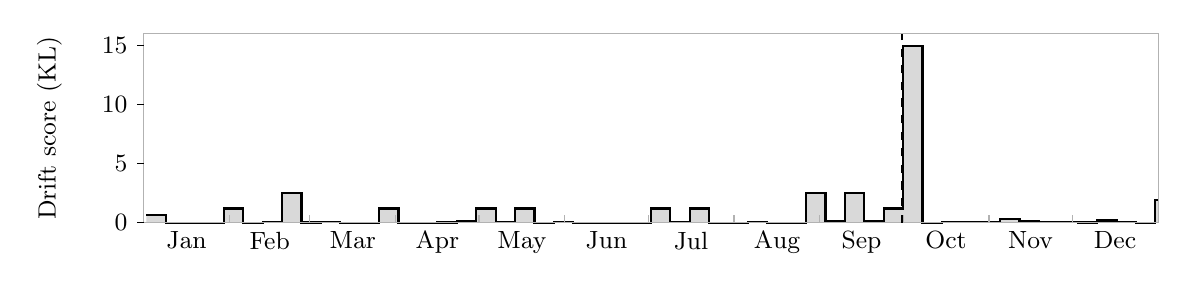
\begin{tikzpicture}[font=\small, x=0.0352cm, y=0.1500cm]
	\fill[black!15] (1.00, 0) -- (1.00, 0.6931) -- (8.00, 0.6931) -- (8.00, 0.0000) -- (15.00, 0.0000) -- (15.00, 0.0000) -- (22.00, 0.0000) -- (22.00, 0.0000) -- (29.00, 0.0000) -- (29.00, 1.2229) -- (36.00, 1.2229) -- (36.00, 0.0000) -- (43.00, 0.0000) -- (43.00, 0.0741) -- (50.00, 0.0741) -- (50.00, 2.5504) -- (57.00, 2.5504) -- (57.00, 0.0248) -- (64.00, 0.0248) -- (64.00, 0.0741) -- (71.00, 0.0741) -- (71.00, 0.0000) -- (78.00, 0.0000) -- (78.00, 0.0000) -- (85.00, 0.0000) -- (85.00, 1.2229) -- (92.00, 1.2229) -- (92.00, 0.0000) -- (99.00, 0.0000) -- (99.00, 0.0000) -- (106.00, 0.0000) -- (106.00, 0.0304) -- (113.00, 0.0304) -- (113.00, 0.1542) -- (120.00, 0.1542) -- (120.00, 1.2229) -- (127.00, 1.2229) -- (127.00, 0.0741) -- (134.00, 0.0741) -- (134.00, 1.2229) -- (141.00, 1.2229) -- (141.00, 0.0000) -- (148.00, 0.0000) -- (148.00, 0.0741) -- (155.00, 0.0741) -- (155.00, 0.0000) -- (162.00, 0.0000) -- (162.00, 0.0000) -- (169.00, 0.0000) -- (169.00, 0.0000) -- (176.00, 0.0000) -- (176.00, 0.0000) -- (183.00, 0.0000) -- (183.00, 1.2229) -- (190.00, 1.2229) -- (190.00, 0.0741) -- (197.00, 0.0741) -- (197.00, 1.2229) -- (204.00, 1.2229) -- (204.00, 0.0000) -- (211.00, 0.0000) -- (211.00, 0.0000) -- (218.00, 0.0000) -- (218.00, 0.0741) -- (225.00, 0.0741) -- (225.00, 0.0000) -- (232.00, 0.0000) -- (232.00, 0.0000) -- (239.00, 0.0000) -- (239.00, 2.5504) -- (246.00, 2.5504) -- (246.00, 0.1542) -- (253.00, 0.1542) -- (253.00, 2.5504) -- (260.00, 2.5504) -- (260.00, 0.1542) -- (267.00, 0.1542) -- (267.00, 1.2229) -- (274.00, 1.2229) -- (274.00, 14.9581) -- (281.00, 14.9581) -- (281.00, 0.0132) -- (288.00, 0.0132) -- (288.00, 0.0766) -- (295.00, 0.0766) -- (295.00, 0.1042) -- (302.00, 0.1042) -- (302.00, 0.0766) -- (309.00, 0.0766) -- (309.00, 0.3384) -- (316.00, 0.3384) -- (316.00, 0.1157) -- (323.00, 0.1157) -- (323.00, 0.0678) -- (330.00, 0.0678) -- (330.00, 0.0573) -- (337.00, 0.0573) -- (337.00, 0.0248) -- (344.00, 0.0248) -- (344.00, 0.2087) -- (351.00, 0.2087) -- (351.00, 0.0573) -- (358.00, 0.0573) -- (358.00, 0.0000) -- (365.00, 0.0000) -- (365.00, 1.9459) -- (366.00, 1.9459) -- (366.00, 0) -- cycle;
	\draw[thick] (1.00, 0.6931) -- (8.00, 0.6931) -- (8.00, 0.0000) -- (15.00, 0.0000) -- (15.00, 0.0000) -- (22.00, 0.0000) -- (22.00, 0.0000) -- (29.00, 0.0000) -- (29.00, 1.2229) -- (36.00, 1.2229) -- (36.00, 0.0000) -- (43.00, 0.0000) -- (43.00, 0.0741) -- (50.00, 0.0741) -- (50.00, 2.5504) -- (57.00, 2.5504) -- (57.00, 0.0248) -- (64.00, 0.0248) -- (64.00, 0.0741) -- (71.00, 0.0741) -- (71.00, 0.0000) -- (78.00, 0.0000) -- (78.00, 0.0000) -- (85.00, 0.0000) -- (85.00, 1.2229) -- (92.00, 1.2229) -- (92.00, 0.0000) -- (99.00, 0.0000) -- (99.00, 0.0000) -- (106.00, 0.0000) -- (106.00, 0.0304) -- (113.00, 0.0304) -- (113.00, 0.1542) -- (120.00, 0.1542) -- (120.00, 1.2229) -- (127.00, 1.2229) -- (127.00, 0.0741) -- (134.00, 0.0741) -- (134.00, 1.2229) -- (141.00, 1.2229) -- (141.00, 0.0000) -- (148.00, 0.0000) -- (148.00, 0.0741) -- (155.00, 0.0741) -- (155.00, 0.0000) -- (162.00, 0.0000) -- (162.00, 0.0000) -- (169.00, 0.0000) -- (169.00, 0.0000) -- (176.00, 0.0000) -- (176.00, 0.0000) -- (183.00, 0.0000) -- (183.00, 1.2229) -- (190.00, 1.2229) -- (190.00, 0.0741) -- (197.00, 0.0741) -- (197.00, 1.2229) -- (204.00, 1.2229) -- (204.00, 0.0000) -- (211.00, 0.0000) -- (211.00, 0.0000) -- (218.00, 0.0000) -- (218.00, 0.0741) -- (225.00, 0.0741) -- (225.00, 0.0000) -- (232.00, 0.0000) -- (232.00, 0.0000) -- (239.00, 0.0000) -- (239.00, 2.5504) -- (246.00, 2.5504) -- (246.00, 0.1542) -- (253.00, 0.1542) -- (253.00, 2.5504) -- (260.00, 2.5504) -- (260.00, 0.1542) -- (267.00, 0.1542) -- (267.00, 1.2229) -- (274.00, 1.2229) -- (274.00, 14.9581) -- (281.00, 14.9581) -- (281.00, 0.0132) -- (288.00, 0.0132) -- (288.00, 0.0766) -- (295.00, 0.0766) -- (295.00, 0.1042) -- (302.00, 0.1042) -- (302.00, 0.0766) -- (309.00, 0.0766) -- (309.00, 0.3384) -- (316.00, 0.3384) -- (316.00, 0.1157) -- (323.00, 0.1157) -- (323.00, 0.0678) -- (330.00, 0.0678) -- (330.00, 0.0573) -- (337.00, 0.0573) -- (337.00, 0.0248) -- (344.00, 0.0248) -- (344.00, 0.2087) -- (351.00, 0.2087) -- (351.00, 0.0573) -- (358.00, 0.0573) -- (358.00, 0.0000) -- (365.00, 0.0000) -- (365.00, 1.9459) -- (366.00, 1.9459);
	\draw[black!30] (0, 0) rectangle (366, 16);
	\node[below, inner sep=1pt] at (15.5, -0.4800) {Jan};
	\node[below, inner sep=1pt] at (45.5, -0.4800) {Feb};
	\draw[black!30] (31.0, 0) -- (31.0, 0.6400);
	\node[below, inner sep=1pt] at (75.5, -0.4800) {Mar};
	\draw[black!30] (60.0, 0) -- (60.0, 0.6400);
	\node[below, inner sep=1pt] at (106.0, -0.4800) {Apr};
	\draw[black!30] (91.0, 0) -- (91.0, 0.6400);
	\node[below, inner sep=1pt] at (136.5, -0.4800) {May};
	\draw[black!30] (121.0, 0) -- (121.0, 0.6400);
	\node[below, inner sep=1pt] at (167.0, -0.4800) {Jun};
	\draw[black!30] (152.0, 0) -- (152.0, 0.6400);
	\node[below, inner sep=1pt] at (197.5, -0.4800) {Jul};
	\draw[black!30] (182.0, 0) -- (182.0, 0.6400);
	\node[below, inner sep=1pt] at (228.5, -0.4800) {Aug};
	\draw[black!30] (213.0, 0) -- (213.0, 0.6400);
	\node[below, inner sep=1pt] at (259.0, -0.4800) {Sep};
	\draw[black!30] (244.0, 0) -- (244.0, 0.6400);
	\node[below, inner sep=1pt] at (289.5, -0.4800) {Oct};
	\draw[black!30] (274.0, 0) -- (274.0, 0.6400);
	\node[below, inner sep=1pt] at (320.0, -0.4800) {Nov};
	\draw[black!30] (305.0, 0) -- (305.0, 0.6400);
	\node[below, inner sep=1pt] at (350.5, -0.4800) {Dec};
	\draw[black!30] (335.0, 0) -- (335.0, 0.6400);
	\draw (0, 0) -- ++(-0.08cm, 0) node[left] {$0$};
	\draw (0, 5) -- ++(-0.08cm, 0) node[left] {$5$};
	\draw (0, 10) -- ++(-0.08cm, 0) node[left] {$10$};
	\draw (0, 15) -- ++(-0.08cm, 0) node[left] {$15$};
	\node[rotate=90] at (-34, 8) {Drift score (KL)};
	\draw[dashed, thick] (273.75, 0) -- (273.75, 16);
\end{tikzpicture}

		\caption{Signal windows of one week, previous signal window as reference}
		\label{fig:approach:drift_signal_inter_week}
	\end{subfigure}

	\medskip
	\begin{subfigure}{\textwidth}
		\centering
		% generated by notebooks/thesis, do not edit by hand
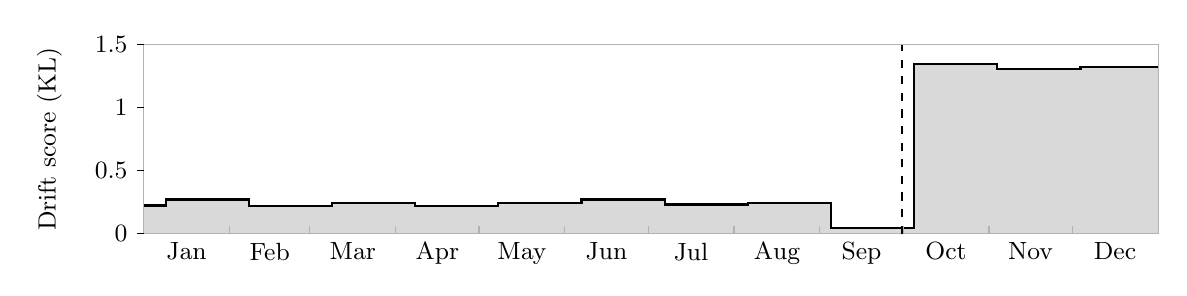
\begin{tikzpicture}[font=\small, x=0.0352cm, y=1.6000cm]
	\fill[black!15] (0.00, 0) -- (0.00, 0.2251) -- (8.00, 0.2251) -- (8.00, 0.2724) -- (38.00, 0.2724) -- (38.00, 0.2232) -- (68.00, 0.2232) -- (68.00, 0.2480) -- (98.00, 0.2480) -- (98.00, 0.2232) -- (128.00, 0.2232) -- (128.00, 0.2480) -- (158.00, 0.2480) -- (158.00, 0.2724) -- (188.00, 0.2724) -- (188.00, 0.2326) -- (218.00, 0.2326) -- (218.00, 0.2480) -- (248.00, 0.2480) -- (248.00, 0.0488) -- (278.00, 0.0488) -- (278.00, 1.3475) -- (308.00, 1.3475) -- (308.00, 1.3078) -- (338.00, 1.3078) -- (338.00, 1.3248) -- (366.00, 1.3248) -- (366.00, 0) -- cycle;
	\draw[thick] (0.00, 0.2251) -- (8.00, 0.2251) -- (8.00, 0.2724) -- (38.00, 0.2724) -- (38.00, 0.2232) -- (68.00, 0.2232) -- (68.00, 0.2480) -- (98.00, 0.2480) -- (98.00, 0.2232) -- (128.00, 0.2232) -- (128.00, 0.2480) -- (158.00, 0.2480) -- (158.00, 0.2724) -- (188.00, 0.2724) -- (188.00, 0.2326) -- (218.00, 0.2326) -- (218.00, 0.2480) -- (248.00, 0.2480) -- (248.00, 0.0488) -- (278.00, 0.0488) -- (278.00, 1.3475) -- (308.00, 1.3475) -- (308.00, 1.3078) -- (338.00, 1.3078) -- (338.00, 1.3248) -- (366.00, 1.3248);
	\draw[black!30] (0, 0) rectangle (366, 1.5);
	\node[below, inner sep=1pt] at (15.5, -0.0450) {Jan};
	\node[below, inner sep=1pt] at (45.5, -0.0450) {Feb};
	\draw[black!30] (31.0, 0) -- (31.0, 0.0600);
	\node[below, inner sep=1pt] at (75.5, -0.0450) {Mar};
	\draw[black!30] (60.0, 0) -- (60.0, 0.0600);
	\node[below, inner sep=1pt] at (106.0, -0.0450) {Apr};
	\draw[black!30] (91.0, 0) -- (91.0, 0.0600);
	\node[below, inner sep=1pt] at (136.5, -0.0450) {May};
	\draw[black!30] (121.0, 0) -- (121.0, 0.0600);
	\node[below, inner sep=1pt] at (167.0, -0.0450) {Jun};
	\draw[black!30] (152.0, 0) -- (152.0, 0.0600);
	\node[below, inner sep=1pt] at (197.5, -0.0450) {Jul};
	\draw[black!30] (182.0, 0) -- (182.0, 0.0600);
	\node[below, inner sep=1pt] at (228.5, -0.0450) {Aug};
	\draw[black!30] (213.0, 0) -- (213.0, 0.0600);
	\node[below, inner sep=1pt] at (259.0, -0.0450) {Sep};
	\draw[black!30] (244.0, 0) -- (244.0, 0.0600);
	\node[below, inner sep=1pt] at (289.5, -0.0450) {Oct};
	\draw[black!30] (274.0, 0) -- (274.0, 0.0600);
	\node[below, inner sep=1pt] at (320.0, -0.0450) {Nov};
	\draw[black!30] (305.0, 0) -- (305.0, 0.0600);
	\node[below, inner sep=1pt] at (350.5, -0.0450) {Dec};
	\draw[black!30] (335.0, 0) -- (335.0, 0.0600);
	\draw (0, 0) -- ++(-0.08cm, 0) node[left] {$0$};
	\draw (0, 0.5) -- ++(-0.08cm, 0) node[left] {$0.5$};
	\draw (0, 1) -- ++(-0.08cm, 0) node[left] {$1$};
	\draw (0, 1.5) -- ++(-0.08cm, 0) node[left] {$1.5$};
	\node[rotate=90] at (-34, 0.75) {Drift score (KL)};
	\draw[dashed, thick] (273.75, 0) -- (273.75, 1.5);
\end{tikzpicture}

		\caption{Signal windows of 30 days, mean of all signal windows as reference}
		\label{fig:approach:drift_signal_inter_month}
	\end{subfigure}
	\caption[Inter-case drift signals of the running example]{%
		Drift signals of the inter-case states of the running example $L_3$ with the KL divergence (Example~\ref{ex:approach:drift_signal_inter}). Each step is a signal window at its drift score, cut at the bounds of the year 2020. The dashed line marks the amount drift on September~30, 2020, 18:00.
		\subref{fig:approach:drift_signal_inter_week}~The first signal window after the drift gets the drift score 14.96. The smaller steps come from feature windows that DBSCAN marks as noise.
		\subref{fig:approach:drift_signal_inter_month}~The three signal windows after the drift lie far from the mean of all signal windows, so the drift shows as a step upwards.}
	\label{fig:approach:drift_signal_inter}
\end{figure}

\begin{example}
	\label{ex:approach:drift_signal_inter}
	We compute two drift signals of the inter-case states of $L_3$ (Example~\ref{ex:approach:clustering_inter}) with the KL divergence (Figure~\ref{fig:approach:drift_signal_inter}).
	\begin{itemize}
		\item First, we choose signal windows of one week and the previous signal window as reference. The 54 signal windows hold 14 feature windows in the median.

		\item The signal window from October~1 reaches the highest drift score 14.96. In this signal window, 71.4\% of the feature windows lie in state~2, which does not occur in the previous signal window.

		\item Ten further signal windows exceed 1. Except the last one, they contain one or two noise feature windows after a signal window without noise. The drift is still 5.9 times higher than the highest of them (2.55).

		\item Second, we choose signal windows of 30 days and the mean of all signal windows as reference. Before the drift, the drift scores lie between 0.22 and 0.27, and after it between 1.31 and 1.35.

		\item Since the amount drift lies at three quarters of the year, only three of the 13 signal windows follow the new process version. They lie far from the reference, so the drift shows as a step upwards, unlike in the intra-case perspective.
	\end{itemize}
\end{example}

The examples show how the reference and the length of the signal windows shape the drift signal. In all three perspectives, the drift creates a state that does not occur before. Therefore, with the previous signal window or the mean of the previous signal windows as reference, the drift signal reaches its highest value in the first or second signal window after the drift. Exceptions are short signal windows with only a few cases or feature windows, whose random fluctuations reach or exceed the drift. With the mean of all signal windows as reference, the drift shows as a step, and the dominant process version decides its direction. Chapter~\ref{chap:eval} evaluates which configurations signal the known drift points in Rheon logs. Table~\ref{tab:approach:running_config} summarizes the configuration of all steps for the three perspectives of the running example.

\begin{table}[tb]
	\centering
	\caption[Configuration of the running example]{%
		Configuration of the running example $L_3$ per perspective. Feature groups are given by their identifiers (Definitions~\ref{def:approach:intra}, \ref{def:approach:resource} and~\ref{def:approach:inter}). The drift signals use the KL divergence and give the length of the signal windows and the reference (Definition~\ref{def:approach:drift_signal}).}
	\label{tab:approach:running_config}
	\small
	\begin{tabular}{@{}l|>{\raggedright\arraybackslash}p{3.3cm}|>{\raggedright\arraybackslash}p{3.3cm}|>{\raggedright\arraybackslash}p{3.3cm}@{}}
		\hline
		Step           & Intra-case                                                    & Resource                                                       & Inter-case                                                                          \\
		\hline
		Rows           & 24,600 events                                                 & 366 windows of 1 day                                           & 731 windows of 12 h                                                                 \\
		\hline
		Feature groups & \texttt{act\_freqs}, \texttt{df\_counts}, \texttt{current\_act} & \texttt{res\_events}, \texttt{act\_res\_shares}                & \texttt{active\_cases}, \texttt{new\_arrivals}, \texttt{mean\_delta\_t}, \texttt{attr\_means} \\
		\hline
		Columns        & 20                                                            & 24                                                             & 4                                                                                   \\
		\hline
		Scaling        & min-max                                                       & z-score                                                        & z-score                                                                             \\
		\hline
		PCA            & $d = 6$                                                       & $d = 1$                                                        & none                                                                                \\
		\hline
		Clustering     & SOM, $3 \times 3$                                             & k-means, $k = 2$                                               & DBSCAN, $\varepsilon = 0.7$, $\mathit{minPts} = 8$                                  \\
		\hline
		States         & 9                                                             & 2                                                              & 2 and noise                                                                         \\
		\hline
		Drift signals  & 1 day, \texttt{recent}, $h = 7$; 7 days, \texttt{baseline}    & 1 day, \texttt{previous}; 30 days, \texttt{recent}, $h = 3$    & 7 days, \texttt{previous}; 30 days, \texttt{baseline}                               \\
		\hline
	\end{tabular}
\end{table}
